\documentclass{article}
\usepackage{hyperref}
\hypersetup{
    urlcolor=blue,
    citecolor=blue,
    colorlinks=true
%    colorlinks=true
}

%    filecolor=magenta,      
%    urlcolor=cyan,
%    pdftitle={Overleaf Example},
%    pdfpagemode=FullScreen,
%    }
\usepackage{comment}
\usepackage{capt-of}
\usepackage{amsmath}
\usepackage{algorithm}
\usepackage{algpseudocode}
\usepackage{cancel}
\usepackage{amsfonts} 
\usepackage{textcomp}
\usepackage{amssymb}
\usepackage{subfig}
\usepackage{caption}
\usepackage{graphicx}
\usepackage{wrapfig}
\usepackage{float}
\usepackage{cancel}
\usepackage{booktabs}
\usepackage{lipsum}
\usepackage{enumerate}
\usepackage{authblk}
\usepackage{makecell}
\usepackage[a4paper, total={6.5in, 9.5in}]{geometry}
\usepackage[utf8]{inputenc}
\usepackage[]{apacite}
\bibliographystyle{apacite}
\usepackage{lineno}
\usepackage{xcolor}
\linenumbers
\DeclareMathOperator*{\argminA}{arg\,min} 
\title{From episodes to concepts and back: Semantic representations in episodic memory enhance recall and compositional consolidation}
%\title{Extracting semantics for episodic memory in Complementary Learning Systems}
\author[1]{Albert Albesa-González}
\author[1]{Claudia Clopath} 
\affil[1]{Department of Bioengineering, Imperial College London, London, UK}
\begin{document}
\maketitle
\begin{abstract}
\noindent 
\end{abstract}
\section*{Introduction}
The distinction between episodic and semantic memory has been central to cognitive neuroscience since its first formalization \shortcite{tulving_1972}. In its original view, episodic memory captures individual experiences, while semantic memory accumulates generalized knowledge that emerges from repeated exposure to similar episodes \shortcite{squire_2004}. One influential computational explanation for this division is provided by the Complementary Learning Systems (CLS) framework. This theory posits that a fast-learning system (the hippocampal and rest of medial temporal lobe, MTL) specializes in rapidly encoding episodic memories. In contrast, a slow-learning neocortical (CTX) system works in concert with the MTL to consolidate, and generalize memories \shortcite{mcclelland_1995, oreilly_2014}.
\newline\newline
Complementary Learning Systems and other consolidation models have historically emphasized a unidirectional transfer of knowledge from episodic traces (MTL) to semantic schemas (CTX) \shortcite{moscovitch_2021}. In this sense, models of the opposite (cortex-to-hippocampus teaching) have remained widely unexplored, as recently pointed in \shortciteA{liu_2024}. However, humans often remember well-structured material more reliably than random or unfamiliar content, suggesting that top-down, schema-like influences can guide the encoding and retrieval of new events \shortcite{bartlett_1932, alba_1983, lin_2021}. On the neurobiological side, research has identified so-called \textit{concept cells} in the human MTL. These are neurons that fire selectively for particular semantic categories or even specific concepts (such as the famously named \textit{Jennifer Aniston neuron}) \shortcite{quiroga_2005, quiroga_2012, courellis_2024}. Furthermore, regions in the medial temporal lobe such as the hippocampus and the entorhinal cortex have been shown to contain neurons coding for latent elements in the environment. These especially include latents related to space \shortcite{o_1971, fyhn_2004, moser_2008}, but also other forms of complex task structure \shortcite{aronov_2017, sun_2020, zhao_2022}. Finally, the existence of long-range prefrontal-to-hippocampal inhibitory connections suggests that abstract information represented in neocortical areas can be directly conveyed to subcortical regions \shortcite{malik_2022}, with these regions exerting top-down control of subcortical areas during sleep \shortcite{swanson_2020, shin_2024}, typically associated with consolidation. All in all, these results suggest that abstract semantic information can be strongly represented in the Medial Temporal Lobe regions, despite its canonical role in episodic memory.
\newline\newline
While views challenging a strict dichotomy between semantic and episodic memory are almost as old as the semantic-episodic distinction itself \shortcite{mckoon_1986, greenberg_2010, gentry_2024}, we still lack a mechanistic understanding of how or why these two memory systems interact. First, most consolidation models assume that replay from hippocampus to cortex is a faithful reinstatement of cortical activity, often overlooking the biological reality that such replays are inherently noisy and the resulting cortical representations are actively constructed rather than simply copied \shortcite{swanson_2020}. Furthermore, highly semantized pre-existing representations are usually assumed \shortcite{saxe_2019, chrysanthidis_2022} sidestepping how such mappings might arise through local, biologically plausible learning rules in the first place. Another key challenge is reconciling the presence of semantic representations in hippocampus and rest of MTL with attractor models of episodic memory. Semantic representations naturally induce overlapping patterns, which have been known for a very long time to reduce memory capacity. For this reason, consolidation models many times assume hash-like codes or other forms of perfect pattern separation, even when the episodes are conceptually highly overlapping \shortcite{sun_2023, chandra_2025}. NOTE FOR CLAUDIA: CITATIONS WERE THERE, THEY REFER TO THE FULL SENTENCE NOT ONLY END.
\newline\newline
Here, we introduce a model of episodic and semantic memory interaction with two key processes: (i) episodic-to-semantic and (ii) semantic-to-episodic consolidation. Episodic-to-semantic consolidation is associated with the standard gradual transfer of information of episodic regularities into semantic memory. Conversely, episodic-to-semantic consolidation transfers these regularities into the episodic code, actively shaping the representations of future episodes based on previously formed abstractions. This cognitive model is presented together with a biologically-motivated circuit model of how such a cognitive algorithm could be implemented. The circuit, based on canonical models of subcortical-cortical consolidation, learns using only local signals via Hebbian and homeostatic plasticity. We use compositional input with a pre-defined statistical structure, which the neocortical component of the model is able to extract and decompose. These compositional representations are then transferred into the episodic memory system (Medial Temporal Lobe), increasing the semantic content of episodic representations. Our model can explain the formation of concept-like cells in subcortical areas \shortcite{quiroga_2005, quiroga_2012}, the advantage of blocked learning in humans \shortcite{flesch_2018}, and the better recall of memories with semantic content \shortcite{lin_2021}. Altogether, our model suggests that semantic memory can enhance episodic memory by transferring into it semantic representations. Furthermore, the presence of these semantic representations in episodic encoding facilitate the consolidation of concepts of higher complexity in semantic memory, supporting learning of higher-order abstractions. These results extend previous models of unidirectional transfer of information from hippocampus to cortex, pointing to a cooperative mechanism where both memory systems enhance each other.  
\newpage
\section*{Results}
\subsection*{A Dual Cognitive-Circuit Model of Semantic and Episodic Memory}
\begin{figure}[h!]
    \centering
    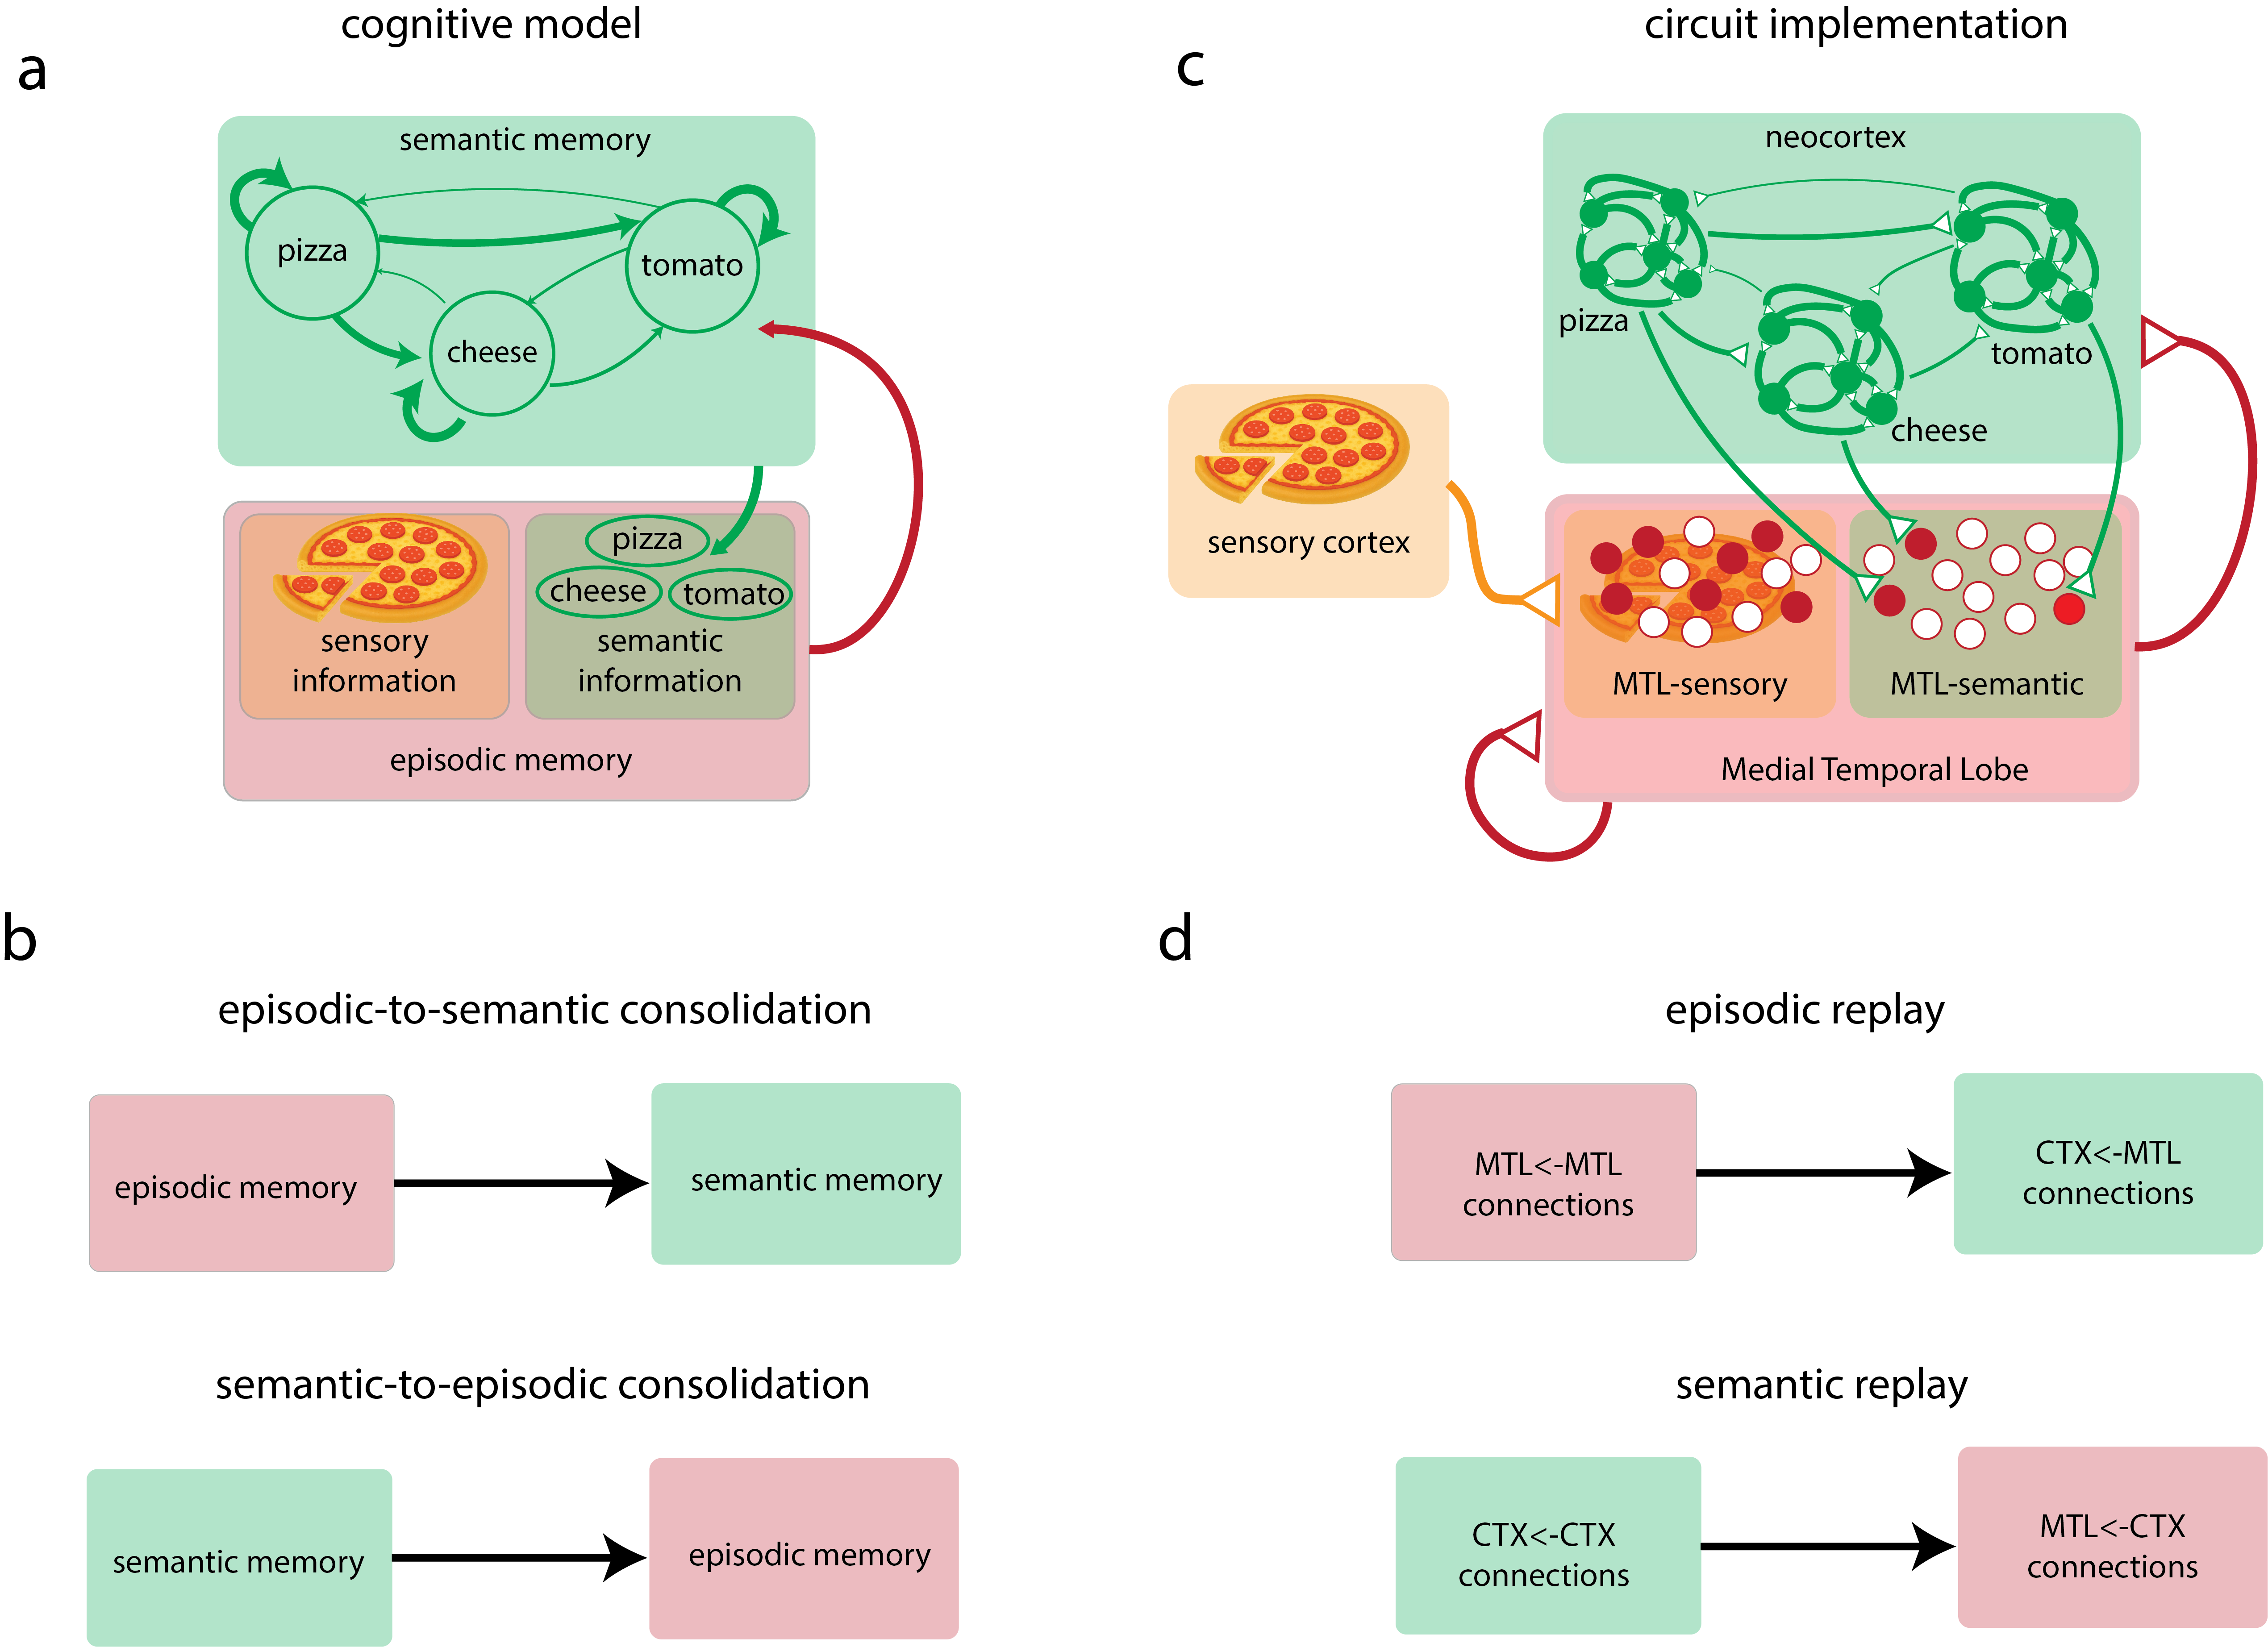
\includegraphics[width=\linewidth]{Figures/Figure_1.png}
    \caption{\textbf{We propose a cognitive model in which semantic memory shapes representations in episodic memory, and an associated circuit implementation.} \textbf{A}: Cognitive model of episodic (red) and semantic (green) memory. Episodic memories integrate both sensory information (orange) and semantic content (green), while semantic memory extracts regularities across episodes. 
\textbf{B}: Schematic of bidirectional consolidation. Episodic-to-semantic consolidation transfers regularities from episodic memory to semantic memory, while semantic-to-episodic consolidation builds semantic representations in episodic memory.  
\textbf{C}: Circuit implementation of the model. Neocortex (CTX) implements semantic memory and Medial Temporal Lobe (MTL) implements episodic memory. MTL is split into neurons primarily receiving input from sensory cortex (MTL-sensory, coding for low-level sensory features) and neurons primarily receiving input from neocortex (MTL-semantic, coding for high-level abstract features). 
\textbf{D}: Mapping of cognitive consolidation processes onto replay mechanisms. Episodic replay corresponds to CTX$\leftarrow$MTL interactions (MTL-to-CTX connections trained during replay), while semantic replay corresponds to MTL-semantic$\leftarrow$CTX interactions (semantic assemblies in CTX driving concept representations in MTL-semantic).}
    \label{fig:diagram}
\end{figure}
\noindent We introduce a cognitive model of semantic and episodic memory, along with an associated neural circuit that could implement it (Fig. \ref{fig:diagram}). We begin with a simple observation: episodic memories often contain both sensory and semantic components. Consider the experience of being served your favorite food: pizza. Across different restaurants and recipes, the visual appearance, smell, and taste may vary widely, leading to diverse sensory inputs and memories. Yet, all of these episodes have something in common: the semantic notion of \textit{pizza} and its main ingredients (crust, cheese, and tomato).
\newline\newline
Our model captures this idea by positing that episodic memories contain two forms of representations: sensory and semantic. In the previous example, an episode involving a pizza (Fig. \ref{fig:diagram}a) integrates the sensory experience (orange), as well as its conceptual representation (green). 
Crucially, even though the model assumes that episodic memory contains semantic representations, the associations formed remain episodic: they link specific events in time.
\newline\newline
In contrast, semantic memory is in charge of extracting regularities across episodes, gradually constructing a dictionary of abstract components. For these two systems to work in concert, we assume two memory transformation processes. First, the semantic system engages in \textit{episodic-to-semantic} consolidation, extracting structure across experiences. Second, semantic memory shapes the representations used by episodic memory, undergoing \textit{semantic-to-episodic} consolidation (Fig. \ref{fig:diagram}b). Through this interaction, early episodic traces, initially dominated by sensory detail, contribute to building semantic knowledge. In turn, semantic knowledge is later used to guide and enrich the formation of new episodic memories. This bidirectional exchange gradually enables episodic representations to combine both sensory and semantic features -as our opening example illustrates.  
\newline\newline
For the circuit implementation, we build upon classic mappings of semantic memory onto neocortical areas (CTX) and episodic memory onto hippocampal and parahippocampal regions (Medial Temporal Lobe, MTL). Following the cognitive model, we subdivide the MTL (episodic memory) into two functional subregions (Fig. \ref{fig:diagram}c), one receiving input from sensory cortex (MTL-sensory), and one from higher-order neocortical areas (MTL-semantic). 
\newline\newline
An important question in the neuroscience of consolidation is how, starting from sensory input, semantic representations can be extracted in CTX (which in the cognitive model corresponds to episodic-to-semantic consolidation). In this sense, the first contribution of our model is proposing that, during \textit{episodic replay}, connections from MTL to CTX are trained to extract repeated elements across episodes, building compositional representations in CTX. Once these representations have formed, CTX forms highly recurrently connected assemblies. These connections learn both what are the different semantic components and what is their causal relationship, completing the process of semantic extraction.
\newline\newline
The second question we explore here is how semantic representations can later be transferred to MTL-semantic (semantic-to-episodic consolidation), forming concept-like representations. To answer this question, in addition to MTL spontaneous activity driving CTX (episodic replay), we include periods in which CTX spontaneous activity drives MTL (\textit{semantic replay}, Fig. \ref{fig:diagram}d), inspired by recent work on top-down control during sleep \shortcite{swanson_2020, shin_2024}. By doing this, neurons in MTL-semantic learn to reproduce the compositional structure of CTX. THIS WAS THE PARAGRAPH I WAS NOT SURE OF. I THINK COMMENTS WERE ON GRAMMAR. CAN YOU TAKE A LOOK AGAIN PLEASE?
\newline\newline
In summary, we propose a model of how episodes and semantics can interact within the brain, supporting both the extraction of compositional knowledge from experiences and the imprinting of conceptual structure onto episodic traces. Next, we will delve deeper into the underlying circuit dynamics that enable these processes, and explore the biological implications and predictions arising from the model.
\subsection*{Episodic replay integrates sensory information into semantic memory}
We first examine how episodic-to-semantic consolidation (Fig. \ref{fig:phase_a}a, left) might be mediated by episodic replay (Fig. \ref{fig:phase_a}a, right). Returning to our pizza example we ask: how can the experience of many episodes containing cheese lead to the formation of a \textit{cheese} representation in CTX? Our circuit model proposes that, by increasing sparsity during replay, MTL can recover common sub-patterns across stored episodes. (Fig. \ref{fig:phase_a}a, right). This promotes the formation of decorrelated neural representations that can be easily learned by neocortex. After abstract cortical mappings have been established in CTX, semantic structure can be further extracted in its recurrent connections.
\newline\newline
To test this idea, we generate sensory input following an Episode Generation Protocol as in \shortciteA{albesagonzalez_2025} (also see Methods). Each episode consists of the simultaneous presentation of a stimulus $A$ (one of $A_1$ to $A_5$) and a stimulus $B$ ($B_1$ to $B_5$) (Fig. \ref{fig:phase_a}b). Each $A_i$ and  $B_j$ is considered a distinct concept, so an episode is defined by a pair $(A_i, B_j)$ -for example, in our illustrative example, $A_1$ could be crust and $B_2$ tomato, so $(A_1, B_2)$ would correspond to an episode with a very basic pizza containing only these two ingredients.  To enrich the semantic structure across concepts, episodes in which $A$ and $B$ share the same sub-index -such as ($A_3$, $B_3$)-  occur 50\% of the time. The remaining combinations are equally distributed in the remaining 50\%. This makes stimulus $A_2$, for example, more semantically related to $B_2$ than to other $B_j$'s. According to the cognitive model, during episodic replay the circuit should therefore build a \textit{dictionary} of concepts in CTX (the full set of $A_i$ and $B_j$) while also capturing the statistical regularities between them (e.g. $A_1$ is more likely to co-occur with $B_1$).
\newline\newline
During episode presentation (\textit{wake}, Algorithm \ref{alg:wake}), MTL$\leftarrow$MTL connections undergo Hebbian plasticity (Algorithm \ref{alg:hebbian}) . During \textit{sleep} (Algorithm \ref{alg:sleep}) random initial activity in MTL evolves via sparse pattern completion (Algorithm \ref{alg:pattern_complete}). Higher sparsity helps uncover sub-patterns of neural activity that correspond to overlaps across different episodes (Fig. \ref{fig:phase_a}c). By reducing the number of active neurons during pattern completion dynamics driving replay, subsets of repeatedly co-active neurons are retrieved (for example those coding for $B_1$, see first timesteps in \ref{fig:phase_a}c). This activity in MTL is projected to CTX via CTX$\leftarrow$MTL connections, which are initially random ($t=0$ in Fig. \ref{fig:phase_a}d). Rapid one-shot plasticity induces an initial receptive field ($t=1000$ in Fig. \ref{fig:phase_a}d) that connects all-to-all between the recovered pattern in MTL and that projected in CTX. Subsequently, affected postsynaptic neurons follow slow Hebbian learning combined with homeostatic plasticity, which refines the original receptive field to match the statistical structure of the input ($t > 1000$, Fig. \ref{fig:phase_a}d). After training, CTX$\leftarrow$MTL connections converge to cover the entire set of episodic concepts $A_1$ to $B_5$ (Fig. \ref{fig:phase_a}e), making neurons in CTX replicate a de-noised and compositional representation of MTL-sensory.
\newline\newline
Pairs of neurons that have formed a receptive field in CTX also follow Hebbian and outgoing homeostatic plasticity (see Methods) in CTX$\leftarrow$CTX connections during \textit{wake}.  Corticocortical connections to capture the conditional firing probabilities \cite{albesagonzalez_2025}. Because cortical neurons have become tuned to individual concepts in episodes (Figs. \ref{fig:phase_a}e and \ref{fig:phase_a}f), capturing conditional firing probabilities is equivalent to 
capturing the statistical structure across concepts (Fig. \ref{fig:phase_a}g).
\newline\newline
Together, these results illustrate how in our circuit model the semantic system (CTX) extracts regularities across overlapping episodic patterns, thereby implementing episodic-to-semantic consolidation. At the synaptic level, cortical feed-forward receptive fields tune neurons to abstract sensory representations, while recurrent connections organize into a block-like structure. This structure contains the semantic information, with intra-block connections representing concepts, and inter-block connections reflecting how much semantically related concepts are. In terms of our pizza example, blocks represent concepts like cheese or tomato, and connections between blocks represent the semantic connection between the ingredients (how likely is to have one in a dish if the other is also present). 
\begin{figure}
    \centering
    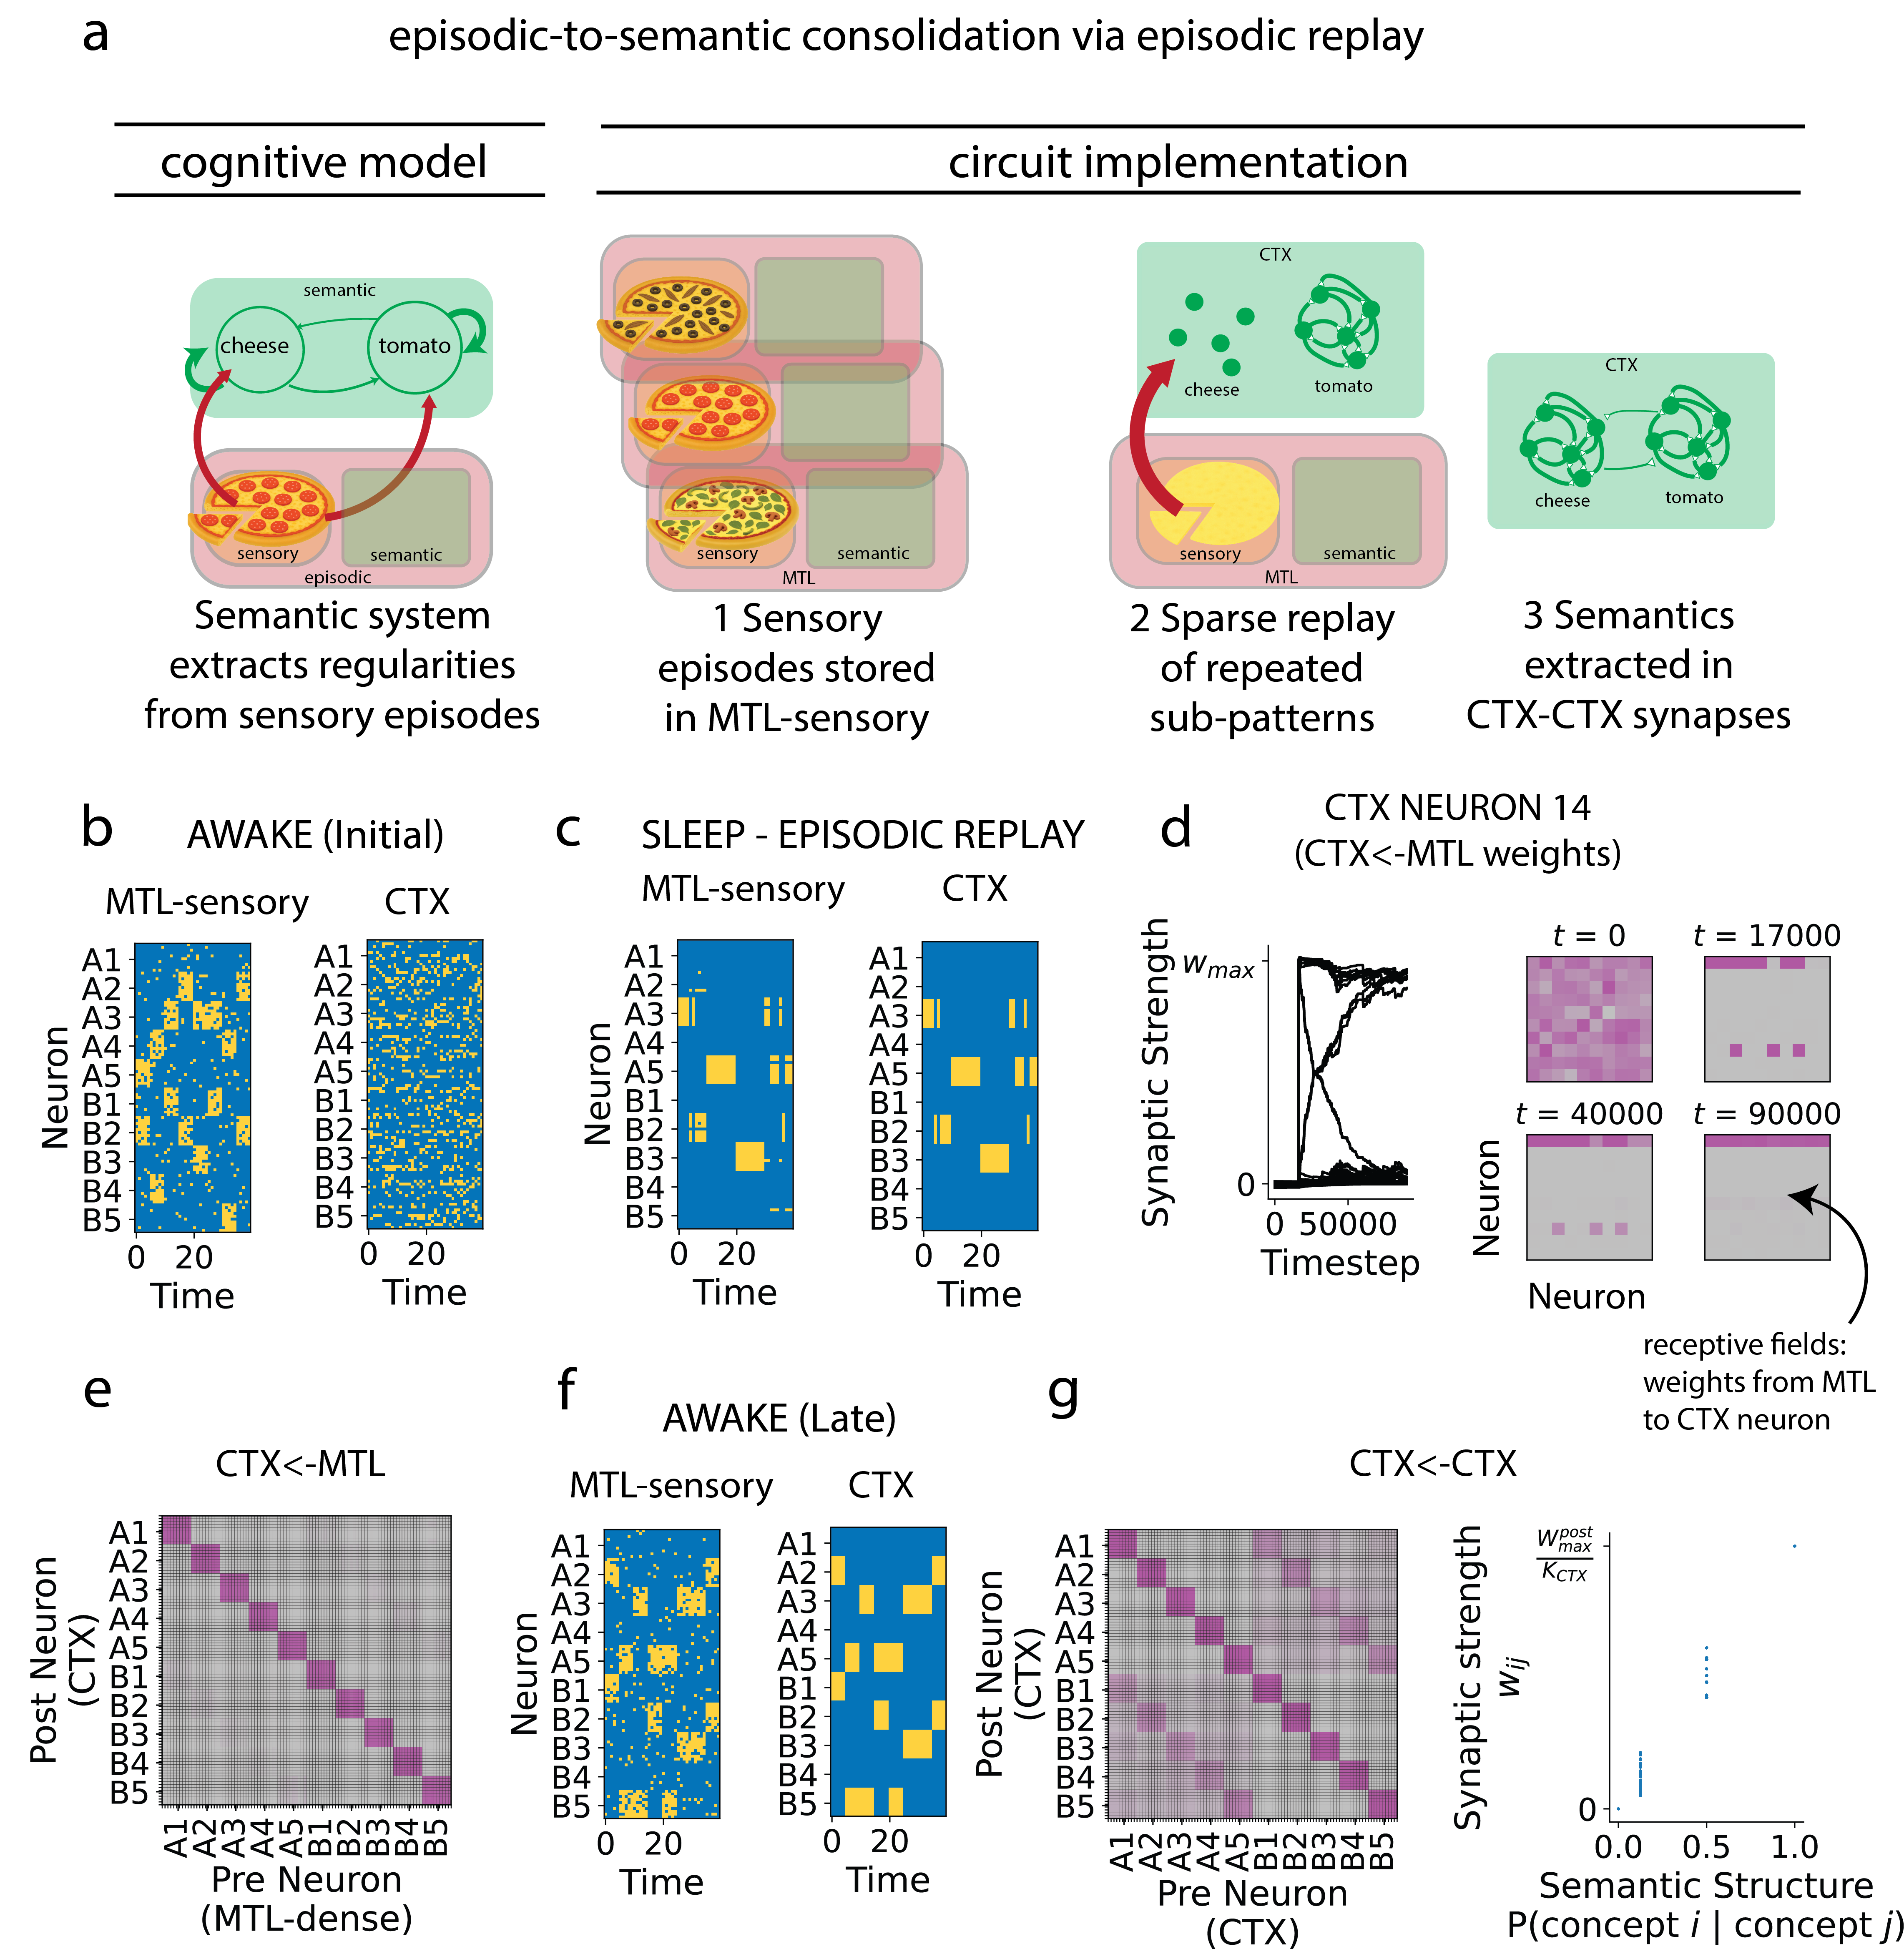
\includegraphics[width=\linewidth]{Figures/Figure_2.png}
\caption{\textbf{Sparse episodic replay creates compositional representations in semantic memory.} \textbf{A}: Episodic-to-semantic consolidation via episodic replay. Cognitive model (left) and circuit implementation (middle/right). Sensory episodes (no semantics extracted yet) are stored in MTL-sensory, replayed sparsely during sleep to uncover overlapping sub-patterns, and then projected to CTX, where compositional semantic structure is extracted in CTX$\leftarrow$MTL (replay) and CTX$\leftarrow$CTX synapses (awake).  
\textbf{B}: Example neuronal activity during wake. Input episodes are sampled following a protocol as described in \shortciteA{albesagonzalez_2025}. To determine MTL-sensory activity, two different concepts (one $A_i \in A$ and one $B_j \in B$ are simultaneously sampled). 50\% of episodes are of form $(A_i, B_{j=i})$, and 50\% $(A_i, B_{j\neq i})$. This makes $A_i$ more semantically related to $B_i$ than the rest of $B$'s. 10 neurons in MTL-sensory code for each concept, and each episode lasts 5 timesteps. At each timestep, $N_\textrm{swaps}= 4$ random neurons that code for the present concepts are turned off, and  $N_\textrm{swaps}= 4$ random neurons that code for non-present concepts are turned on (this introduces noise with a consistent signal-to-noise ratio). CTX activity is driven by random initial CTX$\leftarrow$MTL-sensory connections.
\textbf{C}: Example neuronal activity during episodic replay. Sparse replay in MTL-sensory reveals concept-specific sub-patterns, which create structure in CTX$\leftarrow$MTL-sensory connections via one-shot followed by slow learning.
\textbf{D}: Example CTX neuron receptive field (CTX$\leftarrow$MTL synapses) over training. Initially random connectivity (t = 0) is one-shot driven to represent a replayed presynaptic pattern (t=1000). Then, slow Hebbian and homeostatic plasticity drive statistical learning, uncovering receptive fields that represent semantic components ($t = 1000-50000$). Right: weight dynamics for all synapses of the same neuron.  
\textbf{E}: Final CTX$\leftarrow$MTL weight matrix. Neurons in CTX become tuned to individual concepts ($A_1$–$A_5$, $B_1$–$B_5$), forming a dictionary of abstract components.  
\textbf{F}: Example activity during late wake. CTX neurons now respond selectively to semantic components, showing compositional coding aligned with MTL-sensory input.  
\textbf{G}: Final CTX$\leftarrow$CTX weight matrix (left) and relationship between synaptic strength and semantic structure (right). Recurrent connectivity captures conditional firing probabilities across concepts, organizing into block-like structure encoding semantic associations.}
    \label{fig:phase_a}
\end{figure}
\subsection*{Semantic replay integrates semantic information into episodic memory}
We now investigate the role of semantic replay in semantic-to-episodic consolidation. During semantic-to-episodic consolidation (Fig. \ref{fig:phase_b}a, left), semantic memory should transfer to episodic memory the abstracted representations. In our \textit{pizza} example, after the different ingredients have been consolidated in CTX, these are mapped to MTL-semantic. For example, for someone who has never seen \textit{tomato} sauce, the first episode would not contain a \textit{tomato} explicit representation. However, after semantic-to-episodic consolidation, MTL-semantic would contain neurons explicitly coding for the presence of tomato. From the circuit perspective, MTL-semantic is expected to develop receptive fields that are highly selective to the different assemblies representing concepts in CTX (Fig. \ref{fig:phase_b}a, right).
\newline\newline
To support this process, we now equip the simulated model with semantic replay (Algorithm \ref{alg:sleep}). Semantic replay initializes CTX at random and allows it to recover its own attractors. As in episodic replay, sparsity is increased to isolate patterns corresponding to individual concepts (Fig. \ref{fig:phase_b}b). These patterns are then projected to MTL-semantic, which initially contains random connections. The rationale mirrors that of episodic replay: increasing sparsity produces non-overlapping patterns that can be efficiently learned via competitive learning. As a result, receptive fields in MTL-semantic come to represent individual concepts identified by CTX (Fig. \ref{fig:phase_b}c). Consequently, while MTL-sensory presents a mixed selectivity to different concepts, MTL-semantic neurons show an absolute selectivity to these concepts (Fig. \ref{fig:phase_b}d). This absolute selectivity is reminiscent of concept cells found in the human MTL \shortcite{quiroga_2005, rey_2025}, which we will revisit in the following section.
\newline\newline
We next hypothesize that this type of encoding may support more efficient downstream learning. To test this, we train a classifier to decode the concepts present in an episode from either MTL-sensory or MTL-semantic representations (Fig. \ref{fig:phase_b}f). As a baseline, we also train a model using a one-hot encoding of the concepts present in each episode (\textit{labels} in Figs. \ref{fig:phase_b}f and \ref{fig:phase_b}g). We then compare the classification accuracy after a single epoch, using either sensory or semantic representations, under the assumption that semantic coding may facilitate rapid learning. Initially, the same episode statistics are maintained, and we refer to this as the \textit{In-Distribution} condition. The classifier trained on MTL-semantic representations has a similar performance to training using labels (Fig. \ref{fig:phase_b}g), which is expected given both representations are highly aligned. In contrast, classification using MTL-sensory representations is less accurate, suggesting an advantage of using highly semantic codes in learning.
\newline\newline
We then address the generalization capacity of MTL representations by introducing novel episode statistics. Specifically, we now exclude episodes of the form $(A_i, B_{j=i})$ during learning, and then sample MTL representations exclusively from this type of episode. Thus, the MTL activity used to train the classifiers is obtained with episodes that are \textit{Compositional Out-Of-Distribution}. Again, classifiers trained on MTL-semantic activity match the performance of those trained on labels, while those using MTL-sensory activity perform worse (Fig. \ref{fig:phase_b}h). This highlights the compositional generalization enabled by semantic representations.
\newline\newline
Finally, we examine a more extreme form of generalization by presenting a \textit{Semantic Out-Of-Distribution} condition. Here, episodes are (fixed) random permutations of those shown during training. For this reason, episodes are no longer compositions of $A$ and $B$, and no longer fall under Compositional Out-Of-Distribution. Under these conditions, MTL-semantic representations effectively become a lossy random projection, and no longer provide a reliable basis for decoding (Fig. \ref{fig:phase_b}i). Instead, MTL-sensory become essential for tracking novel input. This shows the two forms of representation serve complementary roles: MTL-semantic supports abstraction and compositional generalization, while MTL-sensory enables flexible adaptation to (semantically) unfamiliar sensory experiences.
\newline\newline
Overall, these results demonstrate that our circuit model, via semantic replay, implements semantic-to-episodic consolidation, as proposed in the cognitive model. This provides a mechanistic account for how semantic representations can be transferred from cortical to subcortical areas, supporting the presence of concept-like cells in MTL \shortcite{quiroga_2005, quiroga_2012}. Moreover, MTL-semantic representations facilitate learning both In-Distribution and Compositional Out-Of-Distribution, while MTL-sensory remains essential for adapting to novel stimuli lacking semantic structure.
\begin{figure}
    \centering
    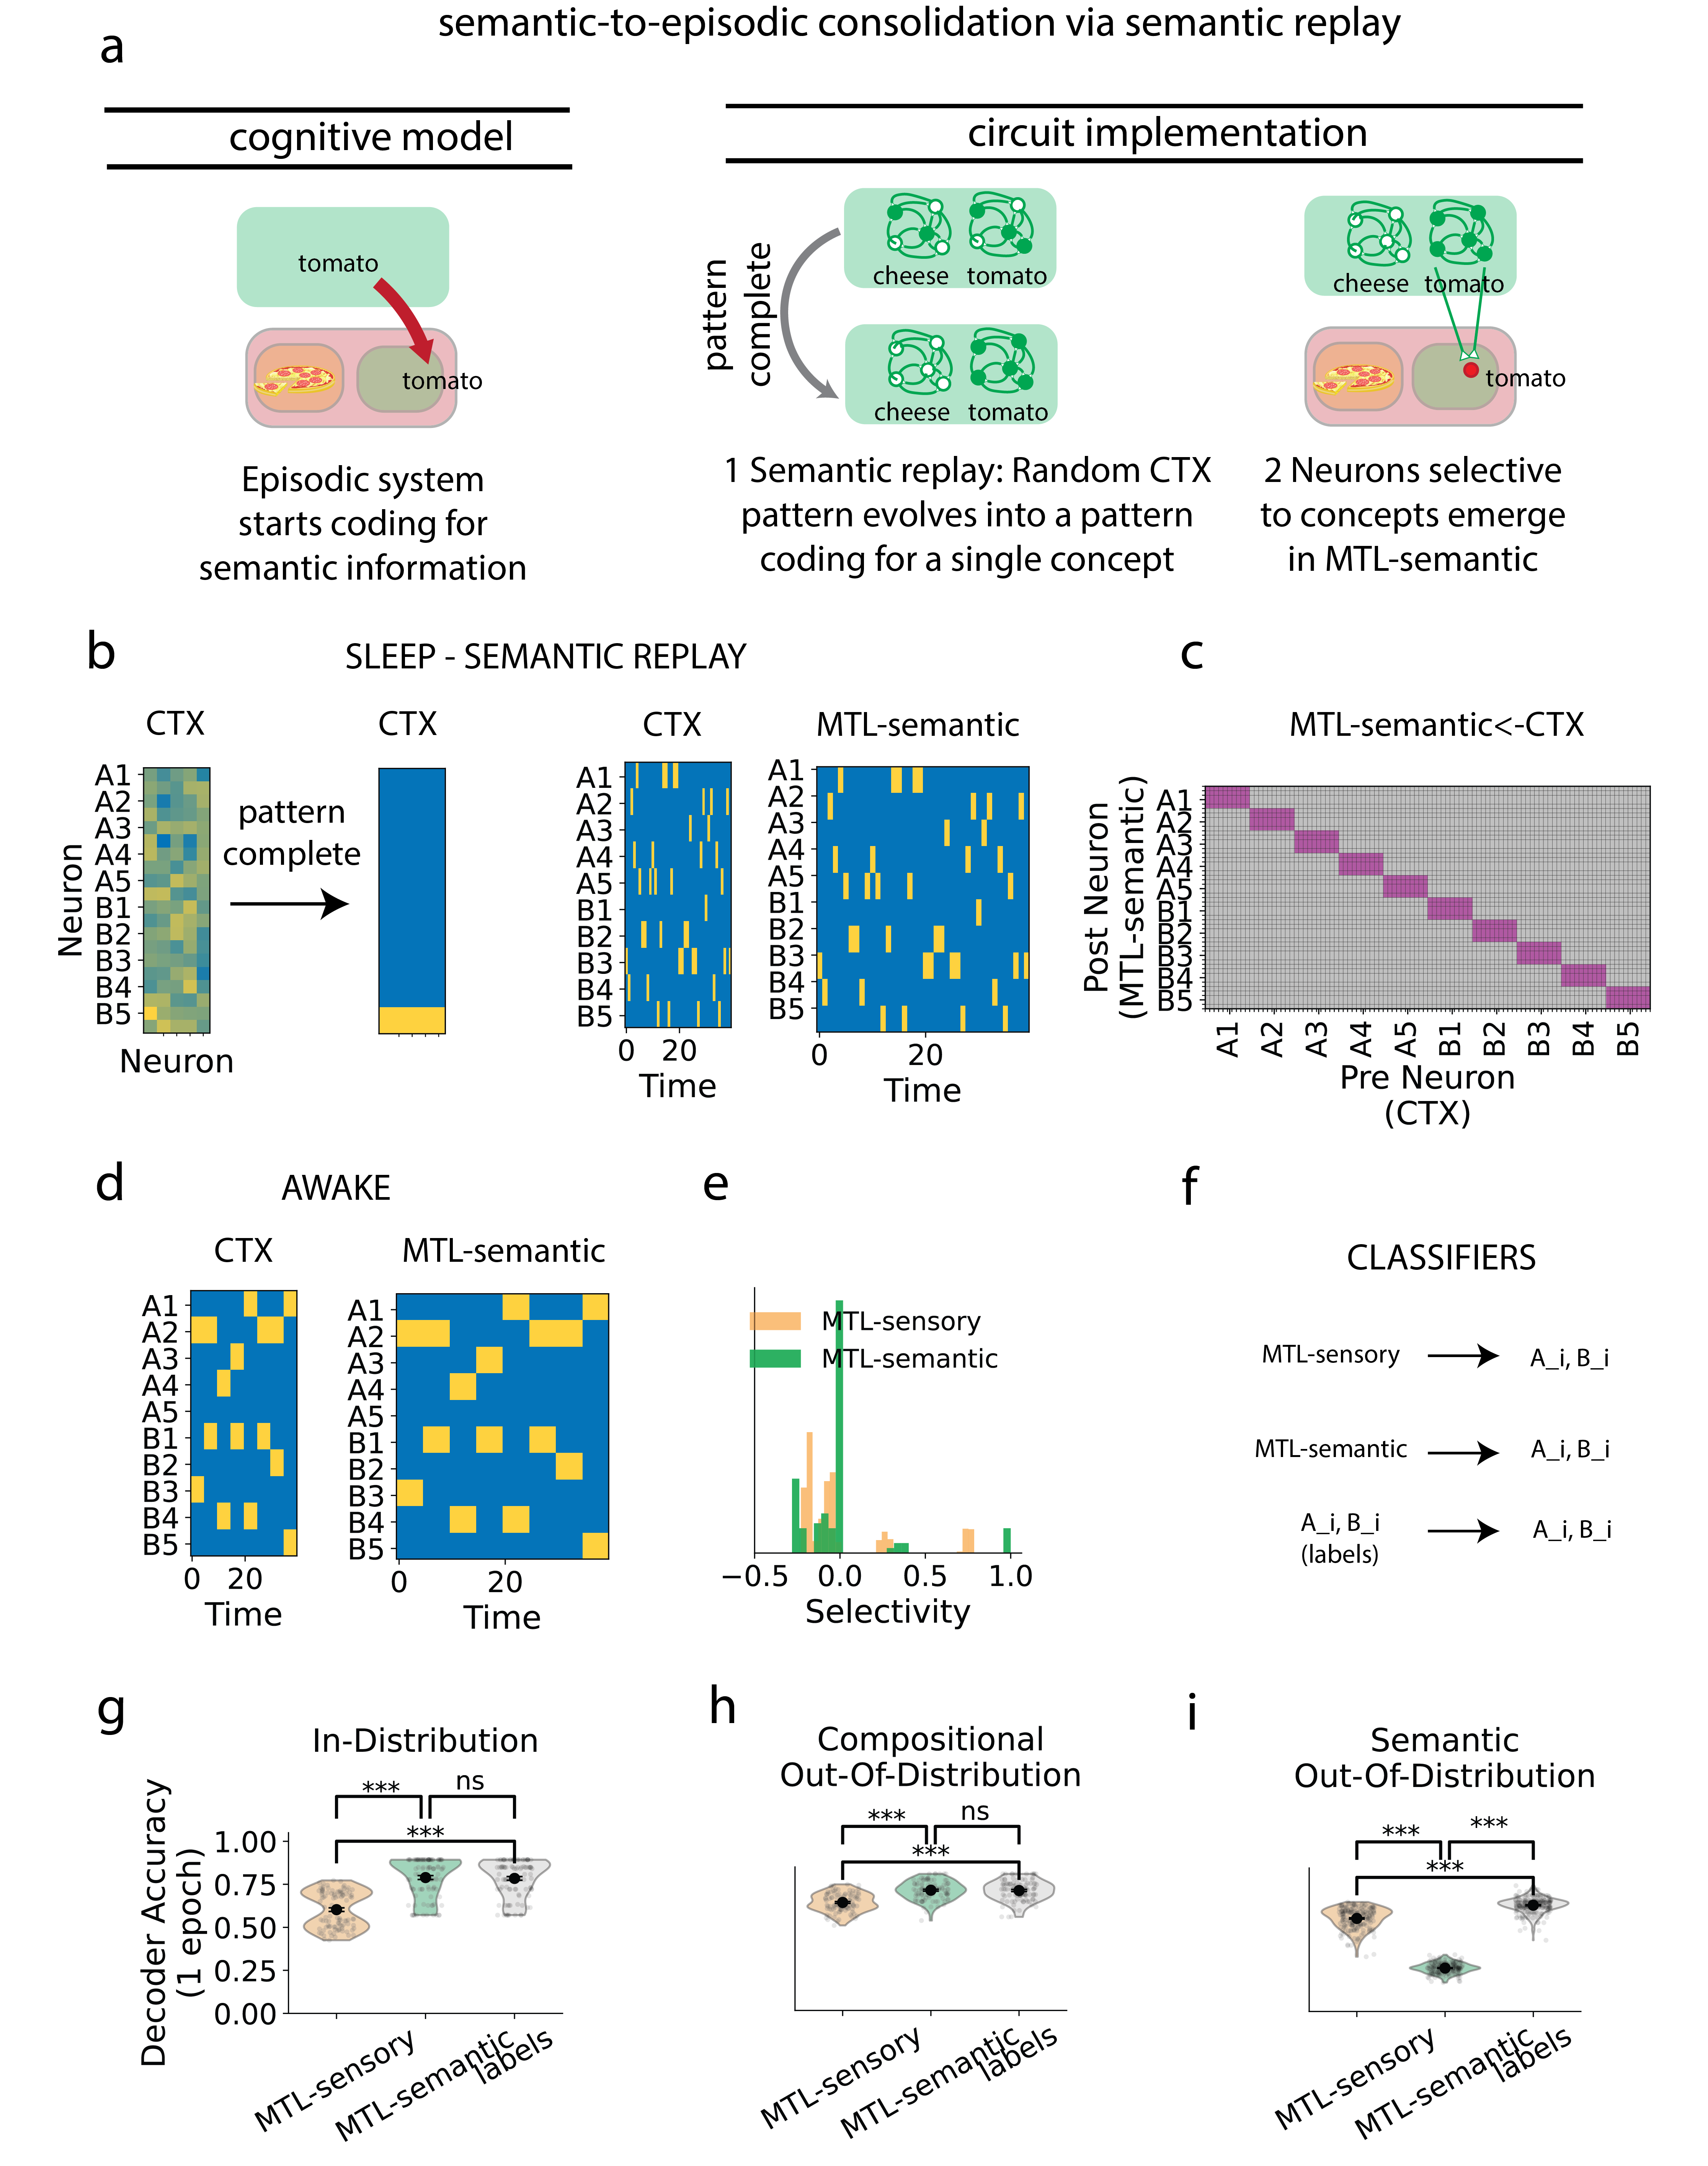
\includegraphics[width=\linewidth]{Figures/Figure_3.png}
\caption{\textbf{Semantic replay forms abstract representations in episodic memory.} \textbf{A}: Semantic-to-episodic consolidation via semantic replay. Cognitive model (left) and circuit implementation (right). During semantic replay, a random CTX pattern converges to a concept-specific attractor, which is then projected to MTL-semantic, creating semantic-specific receptive fields in MTL-semantic and enabling episodic traces to incorporate semantic information.  
\textbf{B}: Example neuronal activity during semantic replay. A random initial CTX state evolves into a complete pattern coding for a single concept, which drives activity in MTL-semantic. A combination of one-shot and slow learning again make neurons that are randomly slightly more sensitive to cortical patterns selective to cortical semantic representations. 
\textbf{C}: Final MTL-semantic$\leftarrow$CTX weight matrix, showing selective mapping from cortical semantic codes to MTL-semantic neurons.}
    \label{fig:phase_b}
\end{figure}
\begin{figure}[t]
  \ContinuedFloat
  \captionsetup{list=off} % don't add a new list-of-figures entry
  \caption{\textit{(continued)} \textbf{D}: Example activity during wake after semantic replay. MTL-semantic neurons now code selectively for concepts, complementing MTL-sensory representations.  
\textbf{E}: Selectivity index of neurons in MTL-sensory and MTL-semantic populations, showing that semantic replay induces sharper concept selectivity in MTL-semantic.  
\textbf{F}: Schematic of classifier training. Classifiers decode concept identity ($A_i$, $B_j$) from either MTL-sensory or MTL-semantic activity.  
\textbf{G--I}: Decoder performance across conditions. \textbf{G}: In-distribution decoding shows both MTL-sensory and MTL-semantic reliably code for concepts. \textbf{H}: Compositional out-of-distribution generalization. MTL-semantic neurons enable successful decoding of unseen concept combinations, while MTL-sensory neurons fail. \textbf{I}: Semantic out-of-distribution generalization. MTL-semantic neurons outperform MTL-sensory neurons in decoding novel semantic relationships. Statistical comparisons: *** $p < 0.001$, ns = not significant.}
\end{figure}
\subsection*{The model explains the formation of concept cells starting from highly mixed representations, which is favored by blocked learning}
We now explore whether the representations formed in the model are consistent with experimental observations in the literature. To this end, we modify the structure of MTL-sensory, which is now a random projection of the patterns used in previous sections (Fig. \ref{fig:experimental_support_1}a and Methods). In the previous MTL-sensory representations, overlaps were completely non-systematic and always due to noise. By randomly projecting the original input, neurons can be activated by different concepts in a persistent manner, (SEN in Fig. \ref{fig:experimental_support_1}a), with MTL-sensory neurons becoming partially tuned to multiple concepts. While the previous arrangement facilitated analysis and visualization, the distribution of neuronal selectivity in the medial temporal lobe is considerably broader than in Fig. \ref{fig:phase_b}e. By projecting the original input, we obtain a more realistic range of selectivity (Fig. \ref{fig:experimental_support_1}b, left, green).
\newline\newline
Our first question is whether concept-like representations still emerge in MTL-semantic with this type of sensory input. We find a clear increase in MTL-semantic selectivity when compared to MTL-sensory (Fig. \ref{fig:experimental_support_1}c, left). However, some concepts collapse into a single representational pattern (see Fig. \ref{fig:experimental_support_1_supp_1}a, right), which hinders the formation of the associated concept neurons. This is a known problem in correlation-based learning, which is still substantially bypassed here (due to the decorrelation from sparse episodic replay), but not completely
\newline\newline
Following this result, we test the hypothesis that -as in humans \shortcite{flesch_2018}- \textit{blocked learning} promotes the acquisition of compositional structures (Figs. \ref{fig:experimental_support_1}b and \ref{fig:experimental_support_1}f, Methods).  Blocked learning involves presenting successive \textit{blocks} of episodes in which one concept is held fixed while the others vary. In contrast, \textit{interleaved learning} maintains the full feature distribution consistently across training. In our simulations, the blocked condition begins with a brief phase in which the network is exposed to sequential batches, each corresponding to a fixed concept (from $A_1$ to $B_5$, Fig. \ref{fig:experimental_support_1}b). We observe that in the model this training structure enhances the selectivity of learned representations (Fig. \ref{fig:experimental_support_1}d, \ref{fig:experimental_support_1}e and Figs. \ref{fig:experimental_support_1_supp_1}a and \ref{fig:experimental_support_1_supp_1}b) and improves accuracy (Fig. \ref{fig:experimental_support_1}f) when using MTL-semantic activity directly as a classifier (see Methods). 
\newline\newline
To better understand these effects, we study the replayed representations in MTL-sensory at the beginning of learning (when semantic representations have not formed yet). Then, we define \textit{concept prototype} (Methods) as a pattern representing the average neuronal activation that corresponds to a fixed concept. By comparing replayed MTL-sensory activity and concept prototypes (Fig. \ref{fig:experimental_support_1}g) we can see how blocked learning promotes replaying activity that is closer to concept prototypes (Fig. \ref{fig:experimental_support_1}h). This makes the initial one-shot receptive fields in CTX$\leftarrow$MTL more selective and less susceptible to representational collapse.
\newline\newline
Our findings demonstrate that our model not only supports the emergence of concept-like representations in MTL, but also highlights the importance of input structure during learning. In particular, blocked learning facilitates the formation of more selective prototype-aligned representations during replay, enhancing the formation of abstract representations in CTX.
\subsection*{Semantic structure explain semantic facilitation of recall and predict more faithful experience replay}
Then, we study the impact of semantic representations on episodic recall. Empirical studies have shown that reducing the semantic component of a stimulus, for example, by scrambling the phase of an image \shortcite{lin_2021} - significantly impairs its memorability (Fig. \ref{fig:experimental_support_2}a). Conceptually, this is akin to the greater difficulty of recalling a random sequence of letters compared to a familiar word of the same length.
\newline\newline
To demonstrate this behaviour in our model, we choose to mimic the original \textit{Intact} vs \textit{Phase-Scrambled} conditions in \shortcite{lin_2021}.  We compared episodic recall performance between a pre-trained network (containing semantic representations, which we call \textit{Intact}), and one in which the MTL-semantic$\leftarrow$CTX connections have been permuted (condition \textit{Scrambled}, to otherwise maintain any other statistic the same, Methods). In both networks, we presented 5 distinct episodes, each lasting 5 timesteps. We then initialized MTL-sensory with one of its states during episode presentation, and allowed all of MTL (sensory and semantic) to follow attractor dynamics, while maintaining sparsity levels to enable recall of full episodes. Recall performance was quantified as the cosine similarity between the recovered pattern and the original (Fig. \ref{fig:experimental_support_2}b and Methods).
\newline\newline
We observe episodes with a clear semantic component are recalled significantly more accurately than those without it, even though both networks have identical sparsity levels (Fig. \ref{fig:experimental_support_2}c). This behaviour persists as the number of stored episodes increases (\textit{Intact} vs. \textit{Scrambled} in Fig. \ref{fig:experimental_support_2}d). Remarkably, the presence of structured correlations in MTL deviates the system from classic memory capacity regimes \shortcite{dubreuil_2014, kang_2023, chandra_2025}. In this sense, here there is no memory cliff (i.e., no sudden drop to near-zero recall after a specific number of episodes). In the absence of semantic representations (\textit{Scrambled}), recall decreases until reaching a plateau (Fig. \ref{fig:experimental_support_2}d, right), but no memory cliff is observed. In the \textit{Intact} condition (semantic representations are present), recall not only avoids a memory cliff but eventually increases, resulting in a U-shaped recall curve. It should be noted, however, this also results in incorrect recall when the number of episodes is very high and episodes are of the form $(A_i, B_{j\neq}i)$ (Fig. \ref{fig:experimental_support_2_supp_1}). Given that all episodes are sampled from the same underlying distribution, this behaviour is consistent with a transition from memorization to generalization. Notably, this behaviour is not exclusive to MTL-semantic, but also extends to MTL-sensory (compare orange curves in \textit{Intact} and \textit{Scrambled}). Because recurrent connections span all-to-all between MTL-semantic and MTL-sensory, the former acts as an error-correcting code for the latter.
\newline\newline
Given that semantic representations error-correct pattern completion during episodic recall, we next hypothesize MTL-semantic could also improve the quality of replayed activity. Until now, during episodic replay, sparsity was increased to decorrelate replay dynamics, yielding sub-patterns shared across episodes rather than full episodes. However, the presence of semantic structure may allow the recovery of episodic patterns, where the number of active neurons matches that observed during \textit{wake}. We tested this by following a similar approach to the \textit{recall} analysis, but starting from random noise instead of a previously seen episode. Because no specific episode was to be recalled, replay performance was measured taking the pattern with the maximum cosine similarity (interpreting the associated pattern as the recalled one). Simulations confirmed the hypothesis, showing a higher overlap between replayed activity and the stored episodes in the \textit{Intact} condition (Fig. \ref{fig:experimental_support_2}e).
\newline\newline
Starting from a validation of previous experimental data (Figs. \ref{fig:experimental_support_2}a and \ref{fig:experimental_support_2}c), we obtain two key predictions of our model: one behavioural and one physiological. The behavioural prediction, derived from Fig. \ref{fig:experimental_support_2}d), is that when episodes contain semantically familiar content, recall initially decreases with increasing memory load but eventually recovers, plateauing at a higher level. The physiological prediction is that replay of semantically structured episodes is more strongly correlated with awake activity than replay of semantically incomprehensible material (Fig. \ref{fig:experimental_support_2}e).
\begin{figure}
    \centering
    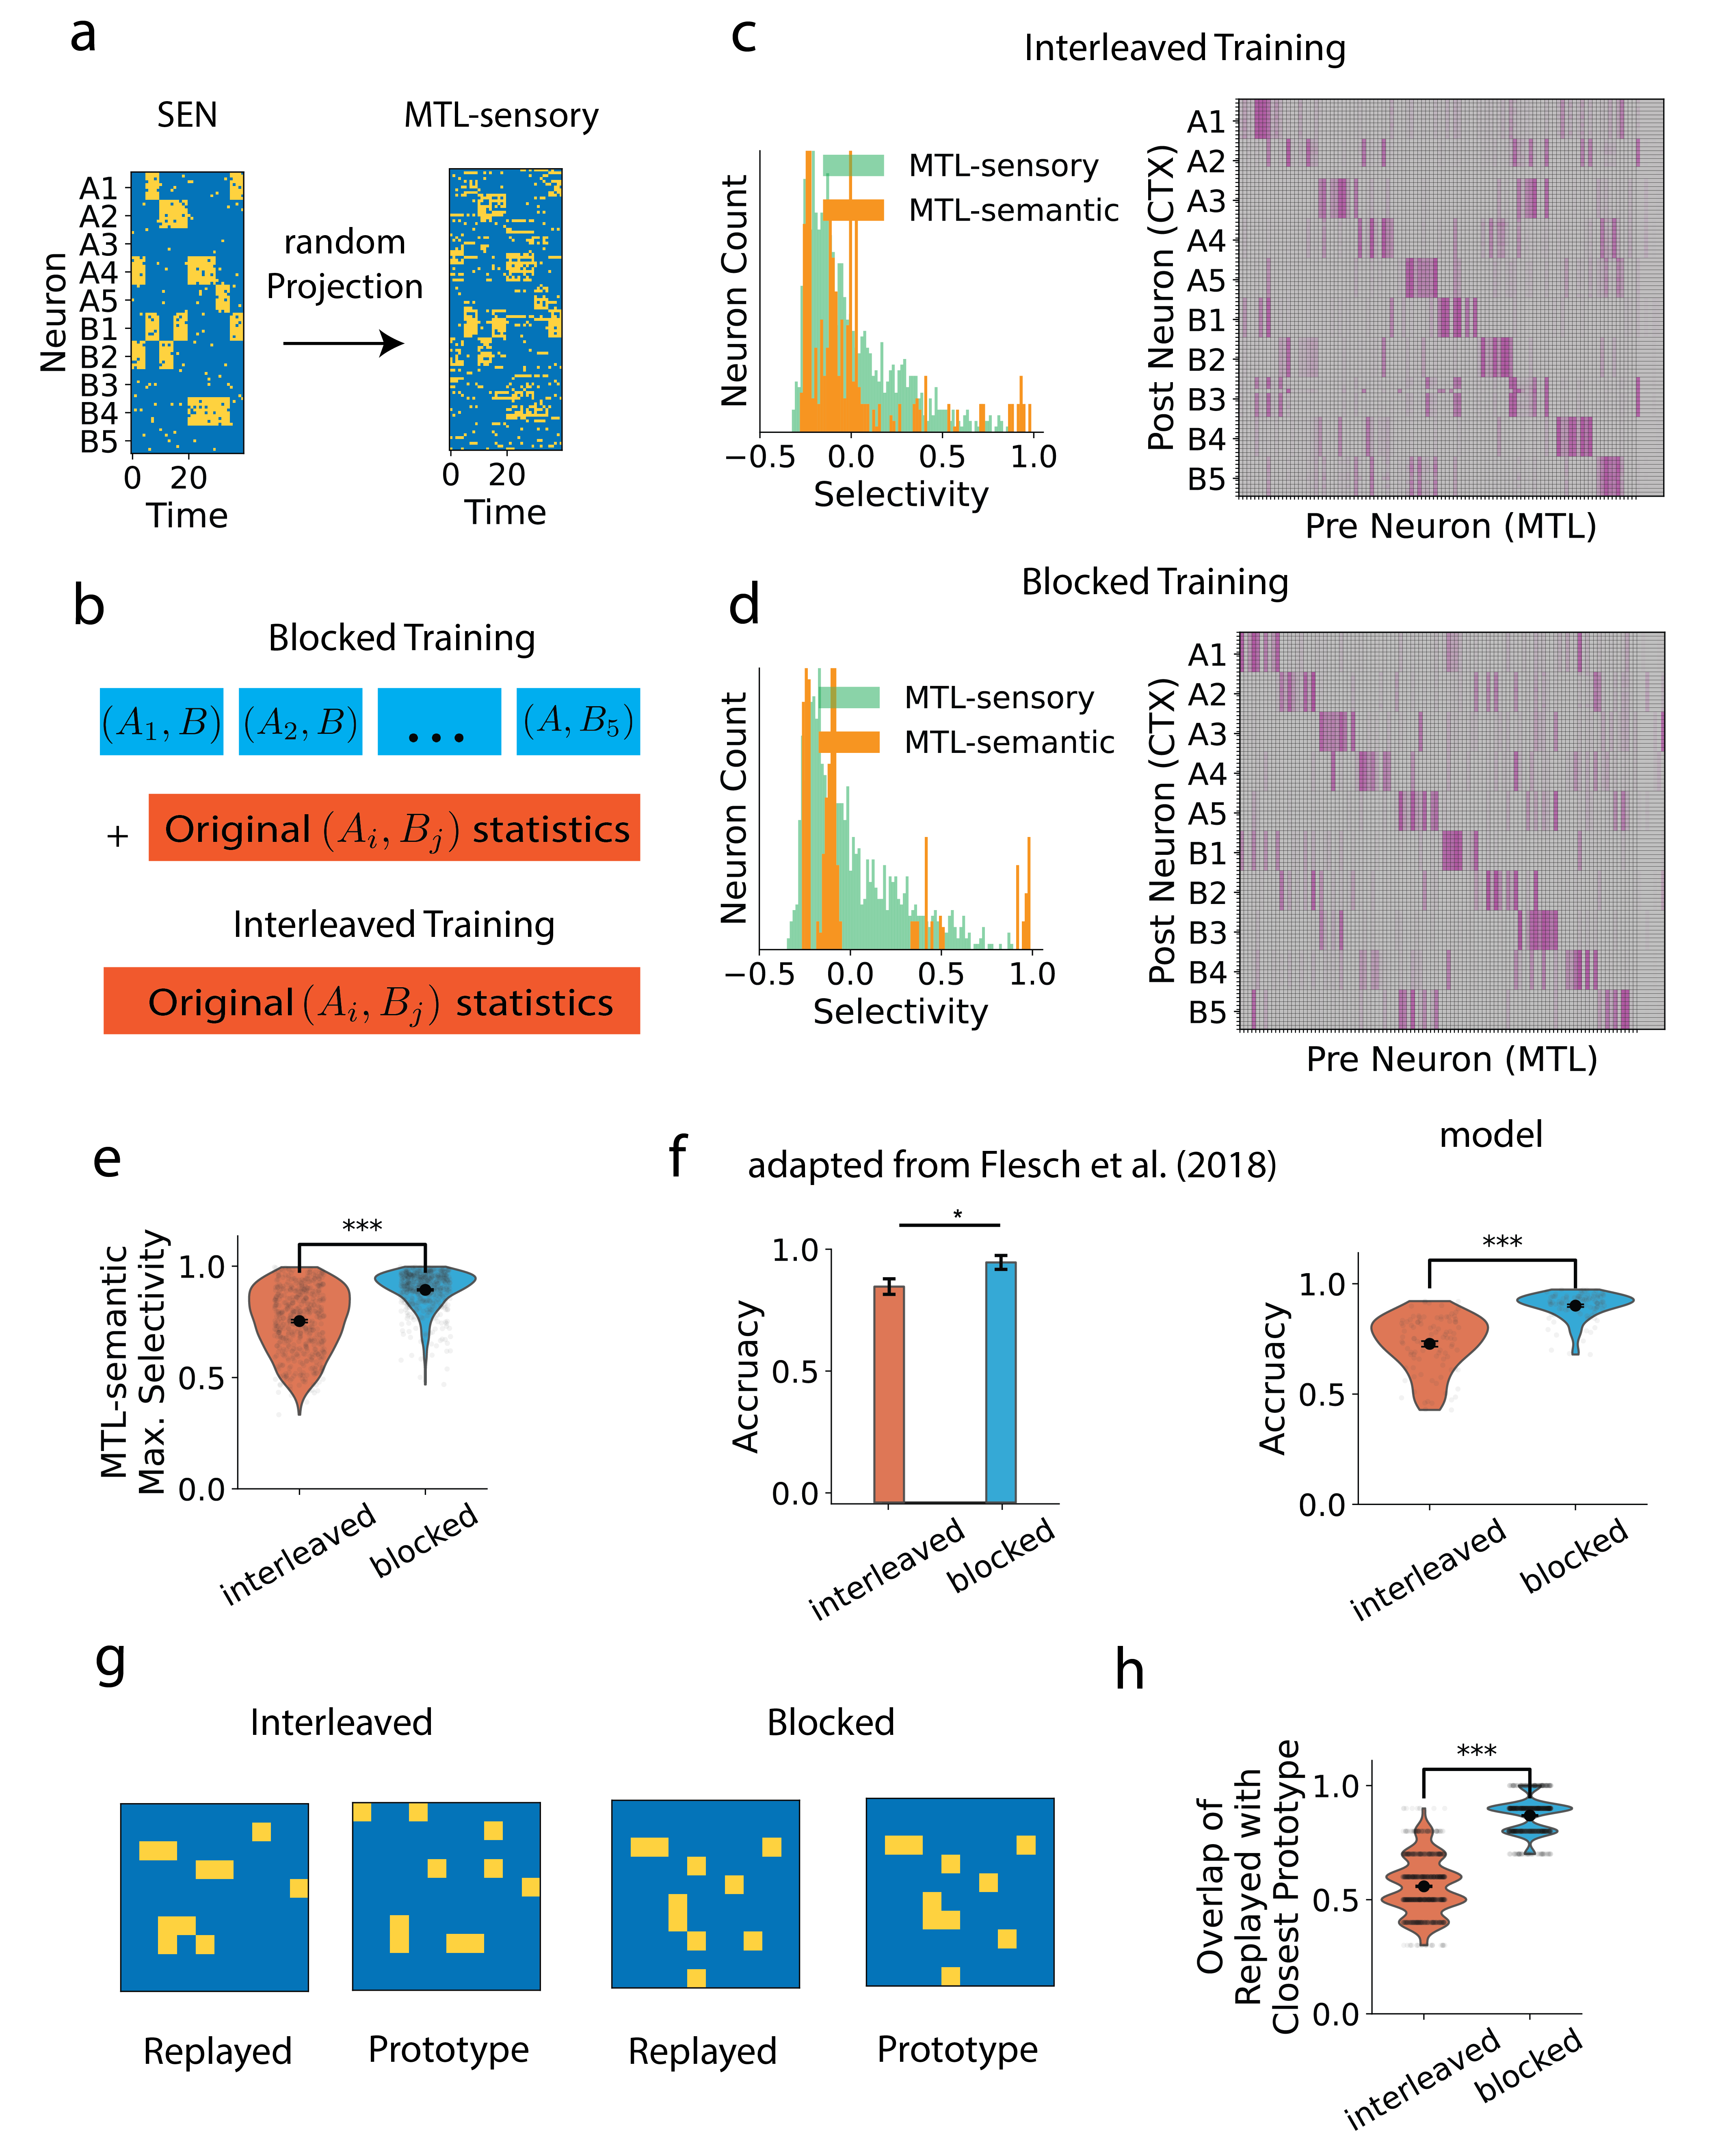
\includegraphics[width=0.95\linewidth]{Figures/Figure_5.png}
\caption{\textbf{Semantic abstraction is favoured by blocked training}\textbf{A}: Example sensory-to-MTL transformation. Sensory input (SEN) is projected through random connections into MTL-sensory, producing noisy but structured population codes.  
\textbf{B}: Training protocols. Interleaved training presents episodes with original ($A_i, B_j$) statistics preserved. Blocked training presents episodes grouped by concept pairs ($A_1,B$, $A_2,B$, ...), disrupting original statistics.  
\textbf{C}: Interleaved training results. Left: selectivity distributions for neurons in MTL-sensory (green) and MTL-semantic (orange). Right: final CTX$\leftarrow$MTL-sensory weight matrix.  
\textbf{D}: Same as \textbf{C} for blocked training. 
\textbf{E}: Quantification of MTL-semantic maximum selectivity across training conditions. Interleaved training produces higher selectivity than blocked training (*** $p<0.001$).  
\textbf{F}: Behavioral and model comparison. Left: human data adapted from Flesch et al.\ (2018), showing reduced accuracy under blocked training. Right: model reproduces this effect, with lower accuracy in blocked vs.\ interleaved training (*** $p<0.001$).}
    \label{fig:experimental_support_1}
\end{figure}
\begin{figure}[t]
  \ContinuedFloat
  \captionsetup{list=off} % don't add a new list-of-figures entry
  \caption{\textit{(continued)} \textbf{G}: Example replayed patterns in MTL-sensory for interleaved (left) and blocked (right). At the right of each replayed pattern, the conceptual prototype activity that is closer to the replayed representation. Under blocked training, replayed patterns align closely with semantic prototypes; under interleaved training, replay is noisier and less aligned. \textbf{H}: Overlap of replay with closest prototype. Blocked training yields higher overlap than interleaved training (*** $p<0.001$).}
\end{figure}
\begin{figure}
    \centering
    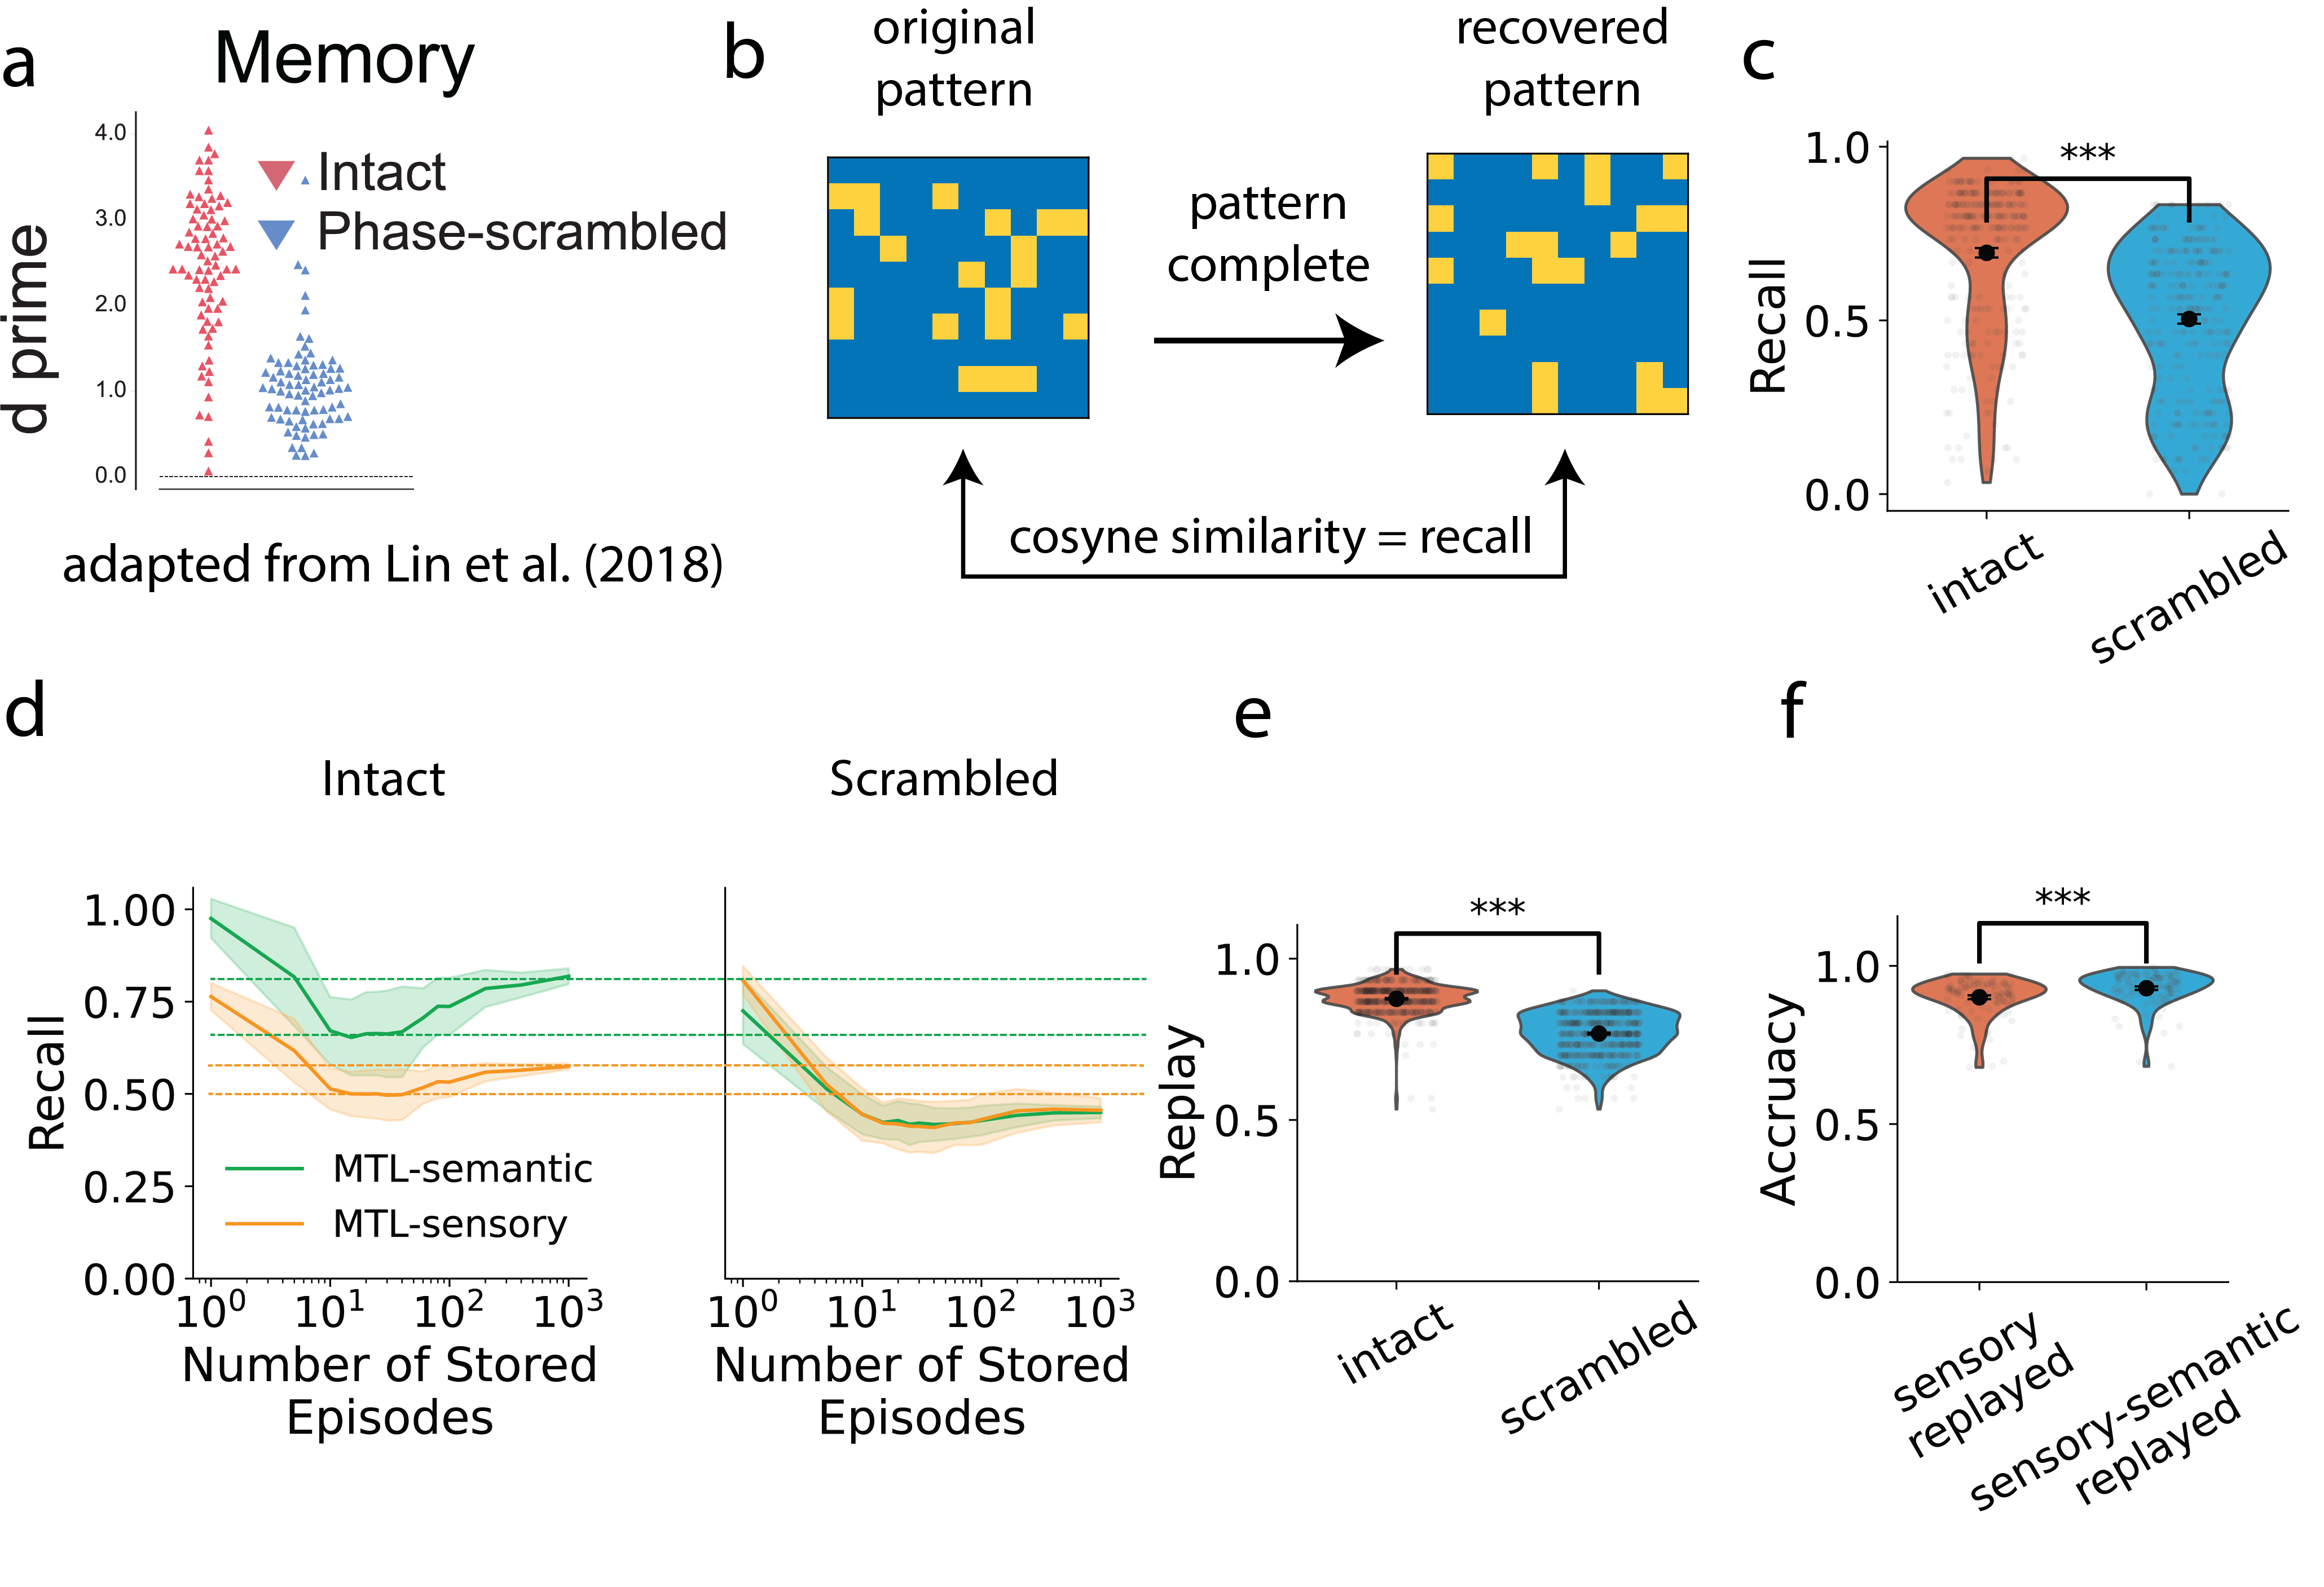
\includegraphics[width=0.95\linewidth]{Figures/Figure_6.png}
\caption{\textbf{Semantic representations structure pattern completion dynamics.} \textbf{A}: Behavioral benchmark. Human data adapted from Lin et al.\ (2018) show reduced memory performance (d-prime) for phase-scrambled compared to intact stimuli.  
\textbf{B}: Schematic of recall measure in the model. Cosine similarity between the original input pattern and the recovered pattern after pattern completion using MTL recurrent connections defines recall accuracy.  
\textbf{C}: Model recall performance. Recall is significantly higher for intact than scrambled patterns (*** $p<0.001$).  
\textbf{D}: Recall as a function of memory load. Due to the correlation structure across patterns, the weight matrix reaches a stable fixed point, resulting in a converging recall performance. In the case of \textit{Intact}, convergence is at a higher value than the performance trough, as a result of semantic representations capturing episodic structure and error-correcting pattern completion dynamics.
\textbf{E}: Replay quality. Cosine similarity of replayed patterns to the closest input episode is higher for intact than scrambled stimuli (*** $p<0.001$).  
\textbf{F}: Accuracy of MTL-semantic representations after extending episodic replay to full (sensory-semantic) replay, compared to initial MTL-semantic accuracy (only sensory representations used during episodic replay). (*** $p<0.001$). Figs. \ref{fig:experimental_support_2}c-e are obtained for the network with best accuracy in Fig. \ref{fig:experimental_support_1_1}f, see Fig. \ref{fig:experimental_support_2_supp} for results on the network with median accuracy (key results still hold).}
    \label{fig:experimental_support_2}
\end{figure}

\subsection*{Episodic replay of sensory-semantic favours higher-order conceptual learning}
Until now, episodic replay has been constrained to increased levels of sparsity, which can decorrelate episodic sub-patterns and uncover compositional structure. CAN YOU CHECK IF THE NOTION OF SPARSE REPLAY WAS CLEAR BY THIS POINT. However, by increasing the number of active neurons one could in principle recover patterns that correspond to higher-order associations of concepts. For example, when presented with multiple episodes containing pizza, the semantic components \textit{crust}, \textit{cheese}, and \textit{tomato} can be replayed together by allowing 3 times more active neurons (Fig. \ref{fig:higher-order}a). Our hypothesis is that, following the results in the previous section, less sparse replay can now be stabilized by semantic representations, allowing CTX to form new concepts that correspond to combinations of previously learned concepts.
\newline\newline
We test the network's ability to use variable sparsity rates during replay to consolidate in CTX categories that are compositions of other categories. To this aim, we define the \textit{Semantic Load} as the ratio between the number of active neurons during replay at a given time and the maximum possible level of sparsity in that region. Intuitively, the semantic load is a measure of how many concepts are present in a representation with a specific sparsity. Then, at each replay event there is a random probability of the semantic load being 1 (one concept replayed) or 2 (two simultaneous concepts replayed) (Fig. \ref{fig:higher-order}b). Thus, an initial MTL pattern follows in any case attractor dynamics driven by recurrent connections, but depending on the maximum number of allowed active neurons falls in an attractor coding for one single or two concepts (top and bottom panels in (Fig. \ref{fig:higher-order}b). MTL activity is further projected to CTX, where a new subregion has been added to drive the discovery of patterns across pairs of concepts.
\newline\newline
As previously, replay with a semantic load of 2, also induces a competition between patterns corresponding to different full episodes -specific combinations $(A_i, B_j)$. Eventually, selective cortical receptive fields emerge for specific episodes (Fig. \ref{fig:higher-order}d). This modifies cortical representations, which now contains during \textit{wake} neurons coding for each $A_i$, for each $B_j$, and for each $(A_i, B_j)$ simultaneously (Fig. \ref{fig:higher-order}c). This completes the process of semantic extraction in CTX, which now stores in its recurrent synapses the full structure of the different compositional units (Fig. \ref{fig:higher-order}e). Because these synapses represent conditional probabilities across concepts, and now there are different levels of abstraction (for example concept $A_1B_1$ implies concept $A_1$, but given concept $A_1$ there is a probability of 1/5 of concept $A_1B_1$), the resulting matrix is highly asymmetric.
\newline\newline
Finally, we investigate whether semantic representations during replay are causally involved in hihger-order learning. This is suggested by our previous results (Fig. \ref{fig:experimental_support_2}e), which showed episodic retrieval from noise was enhanced by the presence of semantic representations. Thus, we again randomly permute MTL-semantic$\leftarrow$CTX connections during higher-order concept learning. Then, we measure the selectivity of formed CTX representations to particular episodes (combinations of two concepts). We observe a significant decrease in episode selectivity in the region of CTX forming higher-order representations (Fig. \ref{fig:higher-order}f), showcasing the relevance of semantic information in consolidating compositions of previously learned concepts.
\newline\newline
In summary, these results demonstrate that varying sparsity during replay enables the network to flexibly traverse the abstraction hierarchy, from single-concept representations to higher-order compositions of multiple concepts. Crucially, the causal perturbation analysis highlights that semantic representations actively scaffold the emergence of higher-order structure. This matches the intuition that learning and retaining new combinations of previously learned concepts is much easier than when the concepts are novel. For example, long-term remembering the ingredients of a pizza that contains never-seen-before regional vegetables is much more complicated than remembering one containing chocolate and honey.
\begin{figure}[h!]
    \centering
    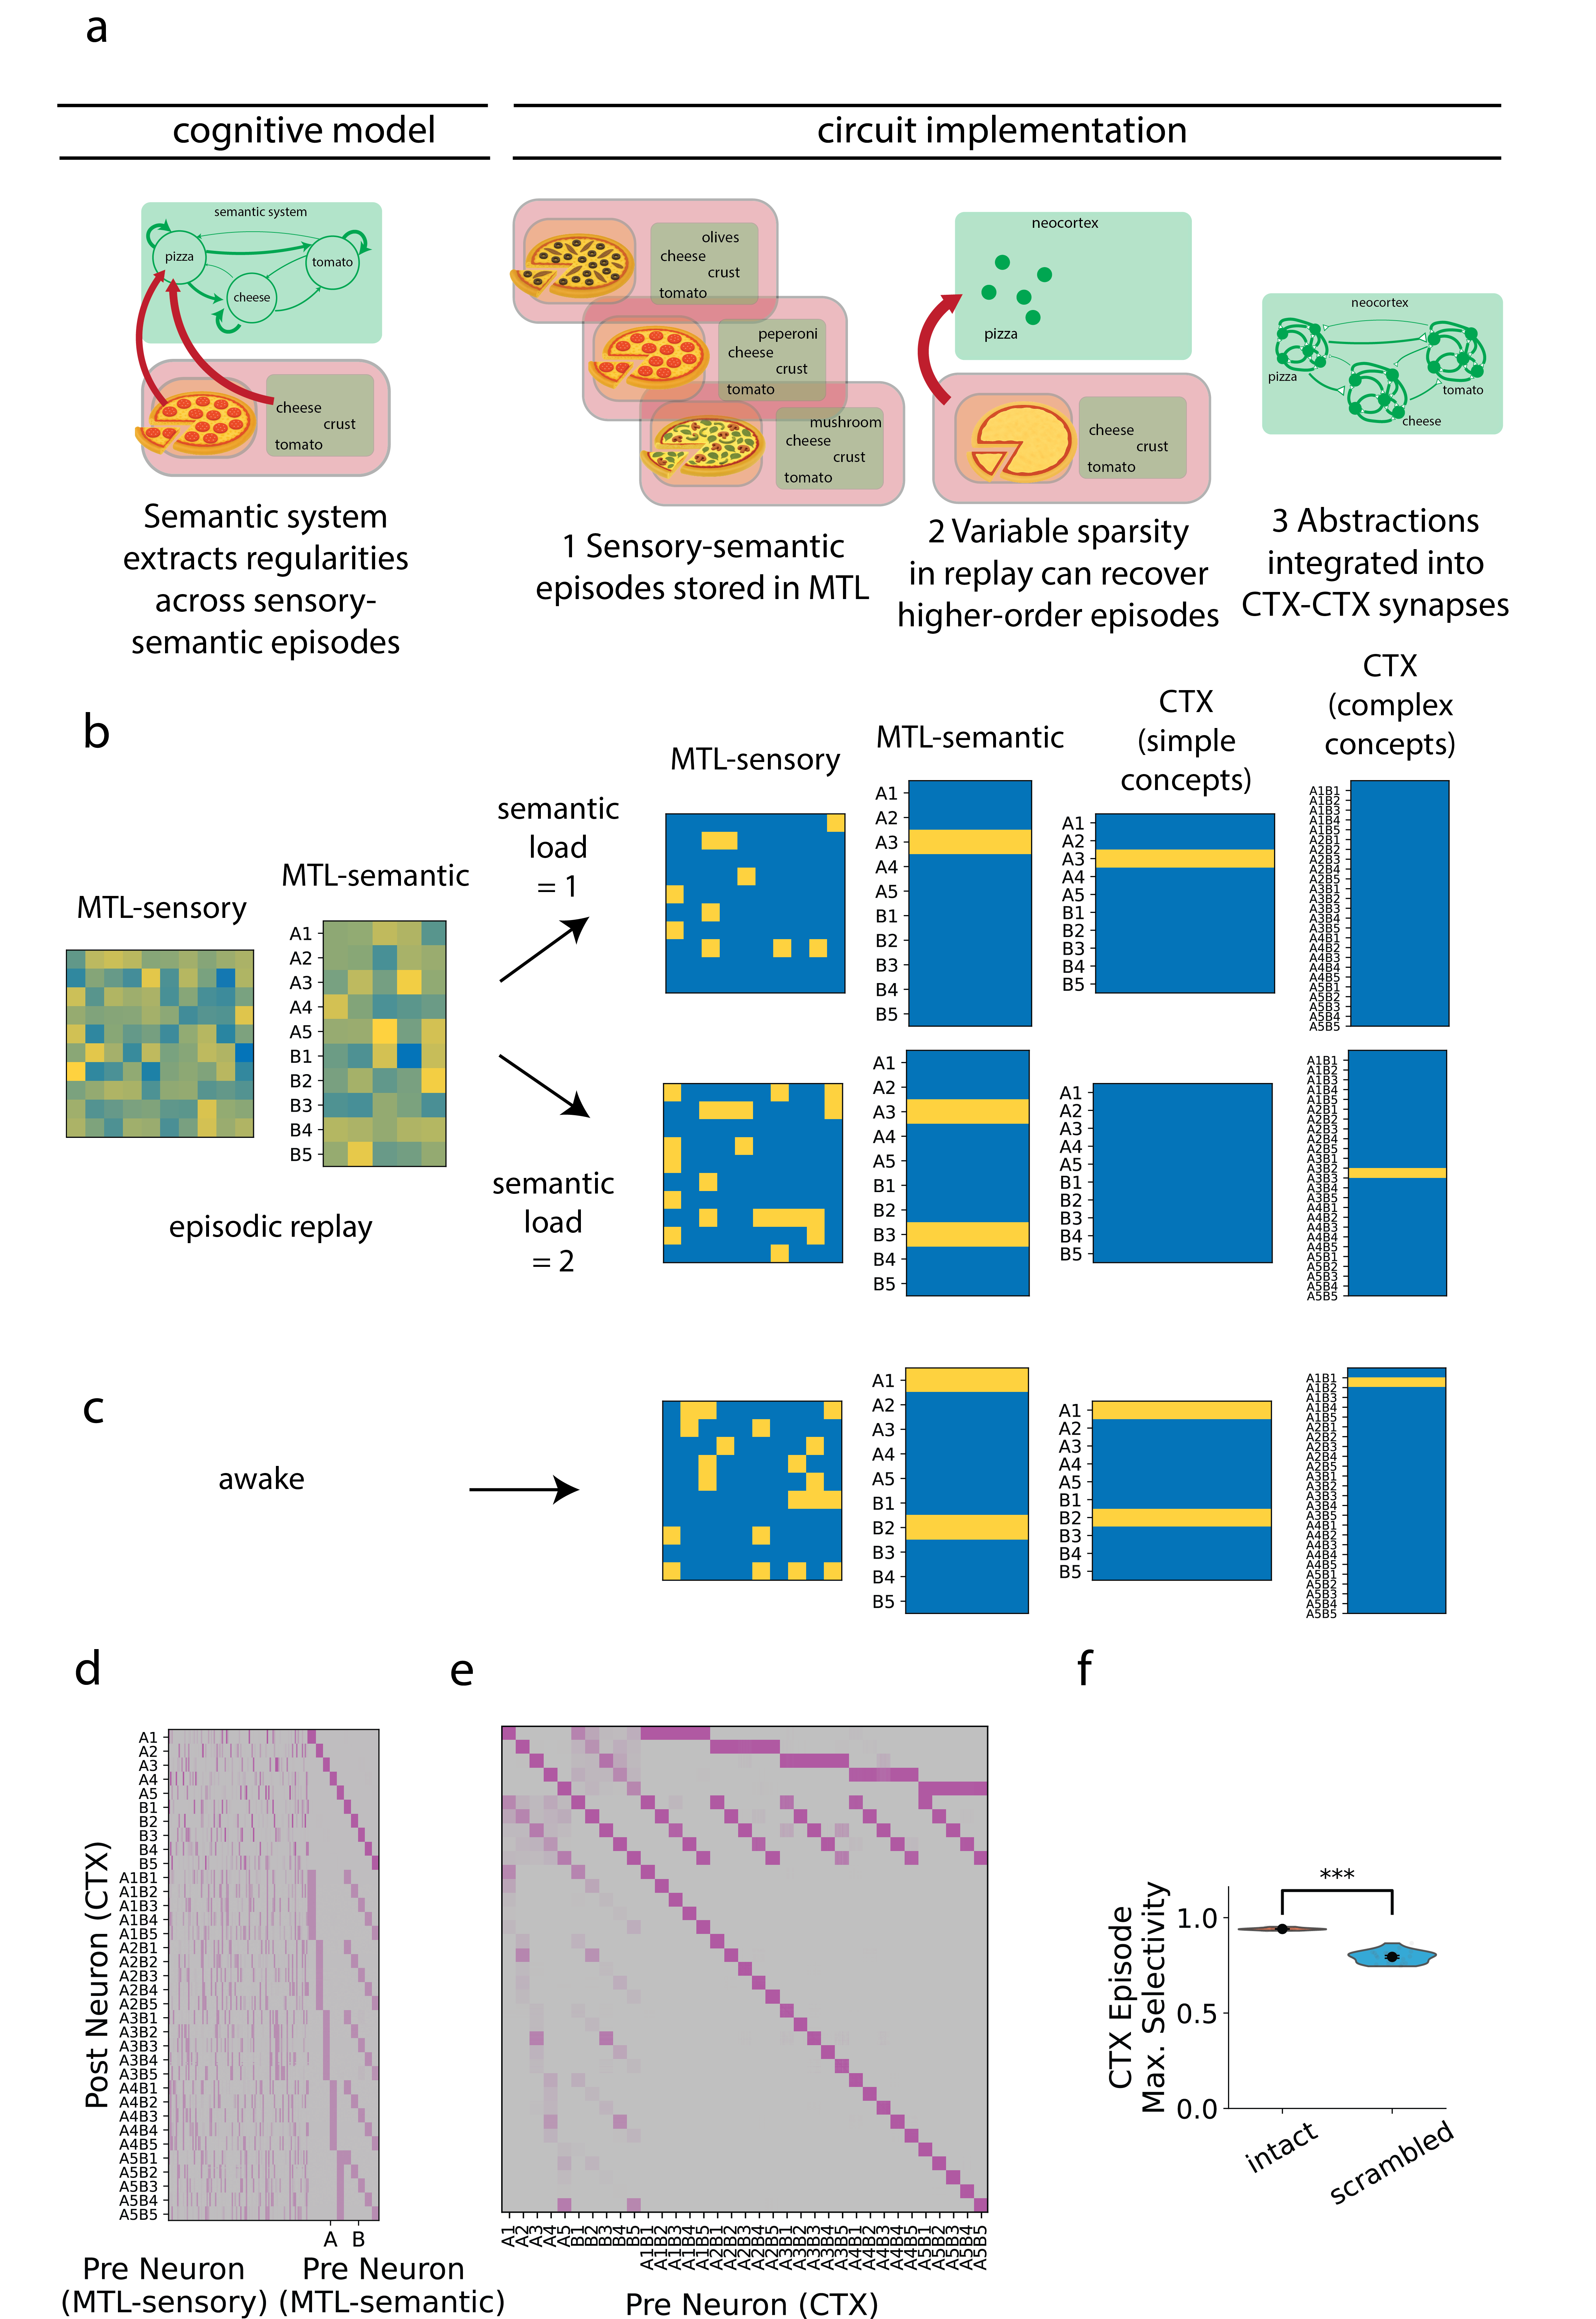
\includegraphics[width=0.95\linewidth]{Figures/Figure_7.png}
\caption{\textbf{Learning higher-order concepts based on simpler representations is facilitated by the presence semantic representations during replay.} \textbf{A}: Cognitive model (left) and circuit implementation (right) of higher-order concept learning. Multiple sensory–semantic episodes are stored in MTL. Variable sparsity during replay (semantic load) allows the recovery of higher-order associations, which are then consolidated into CTX$\leftarrow$MTL and  CTX$\leftarrow$CTX connections.}
    \label{fig:higher-order}
\end{figure}
\begin{figure}[h!]
  \ContinuedFloat
  \captionsetup{list=off} % don't add a new list-of-figures entry
  \caption{\textit{(continued)} \textbf{B}: Example activity during replay with semantic load 1 (top) or 2 (bottom). When one concept is replayed, CTX develops selective coding for single concepts. When two concepts are replayed simultaneously, CTX develops receptive fields for their combinations, supporting higher-order abstractions.  
\textbf{C}: Example activity during wake after training. CTX contains neurons selective to individual concepts $A_i$ and $B_j$, as well as to combinations ($A_i, B_j$).  
\textbf{D}: Final CTX$\leftarrow$MTL weight matrix. Cortical neurons integrate inputs from both MTL-sensory and MTL-semantic at different levels of abstraction.
\textbf{E}: Final CTX$\leftarrow$CTX weight matrix, showing asymmetric recurrent connectivity consistent with conditional probabilities across concepts. Block-like and diagonal substructures capture both simple and compositional units.  
\textbf{F}: Causal role of semantic replay. Random permutation of MTL-semantic$\leftarrow$CTX connections during higher-order learning significantly reduces episode selectivity in CTX (*** $p<0.001$), demonstrating that semantic representations actively scaffold the emergence of compositional structure. Figs. \ref{fig:experimental_support_2}b-e are obtained for the network with best accuracy in Fig. \ref{fig:experimental_support_2}f, see Fig. \ref{fig:higher_order_supp} for results on the network with median accuracy (key results still hold).}
\end{figure}
\clearpage
\begin{comment}
\subsection*{Episodic replay integrates sensory-semantic information into semantic memory: semantic refinement of cortical engrams}
During phase C of learning, the circuit is probed to refine cortical representations with the semantic input received from MTL-semantic (Fig. \ref{fig:phase_c}a). In this sense, neurons in CTX are expected to expand their receptive fields, now receiving meaningful projections from both MTL-sensory and MTL-semantic. In order to allow conjunctions of sensory and semantic patterns to be replayed together, both sub-regions in MTL share recurrent connectivity, storing the overall MTL activity with Hebbian plasticity. Similarly to phase A, the replayed activity corresponds to sub-patterns of stored episodes, but note how now within this sparser sub-patterns there is both a sensory and a semantic component. Mechanistically, phase C is equivalent to phase A, but now makes use of the joint sensory-semantic representations present in MTL.
\newline\newline
To test the degree in which this happens in the circuit, we first examine the MTL activity replayed during sleep. As in previous sections, sparsity during sleep is higher than during wakefulness, which allows recovering sensory-semantic sub-patterns (Fig. \ref{fig:phase_c}b). Note how, due to no distinction at the connectivity level (all MTL is a single recurrent lawyer) sensory and semantic patterns are coupled. 
\newline\newline
Next, we examine the evolution of the CTX$\leftarrow$MTL connectivity. During learning phase A, selective connections from MTL-sensory to CTX where already developed (Fig. \ref{fig:phase_a}f). Given that sensory and semantic activity is coupled during replay, now MTL-sensory drives activity in cortical neurons, which passively become tuned to MTL-semantic (Fig. \ref{fig:phase_c}c).
\newline\newline
While this last learning phase might seem redundant, in the next section we will see how it is crucial for cortical neurons to be able to read from MTL-semantic. In more realistic setups with lower selectivity in MTL-sensory, recall is more noisy in MTL-sensory than in MTL-semantic. This would make retrieval of previous experiences harder when only sensory information can be read from MTL.
\begin{figure}
    \centering
    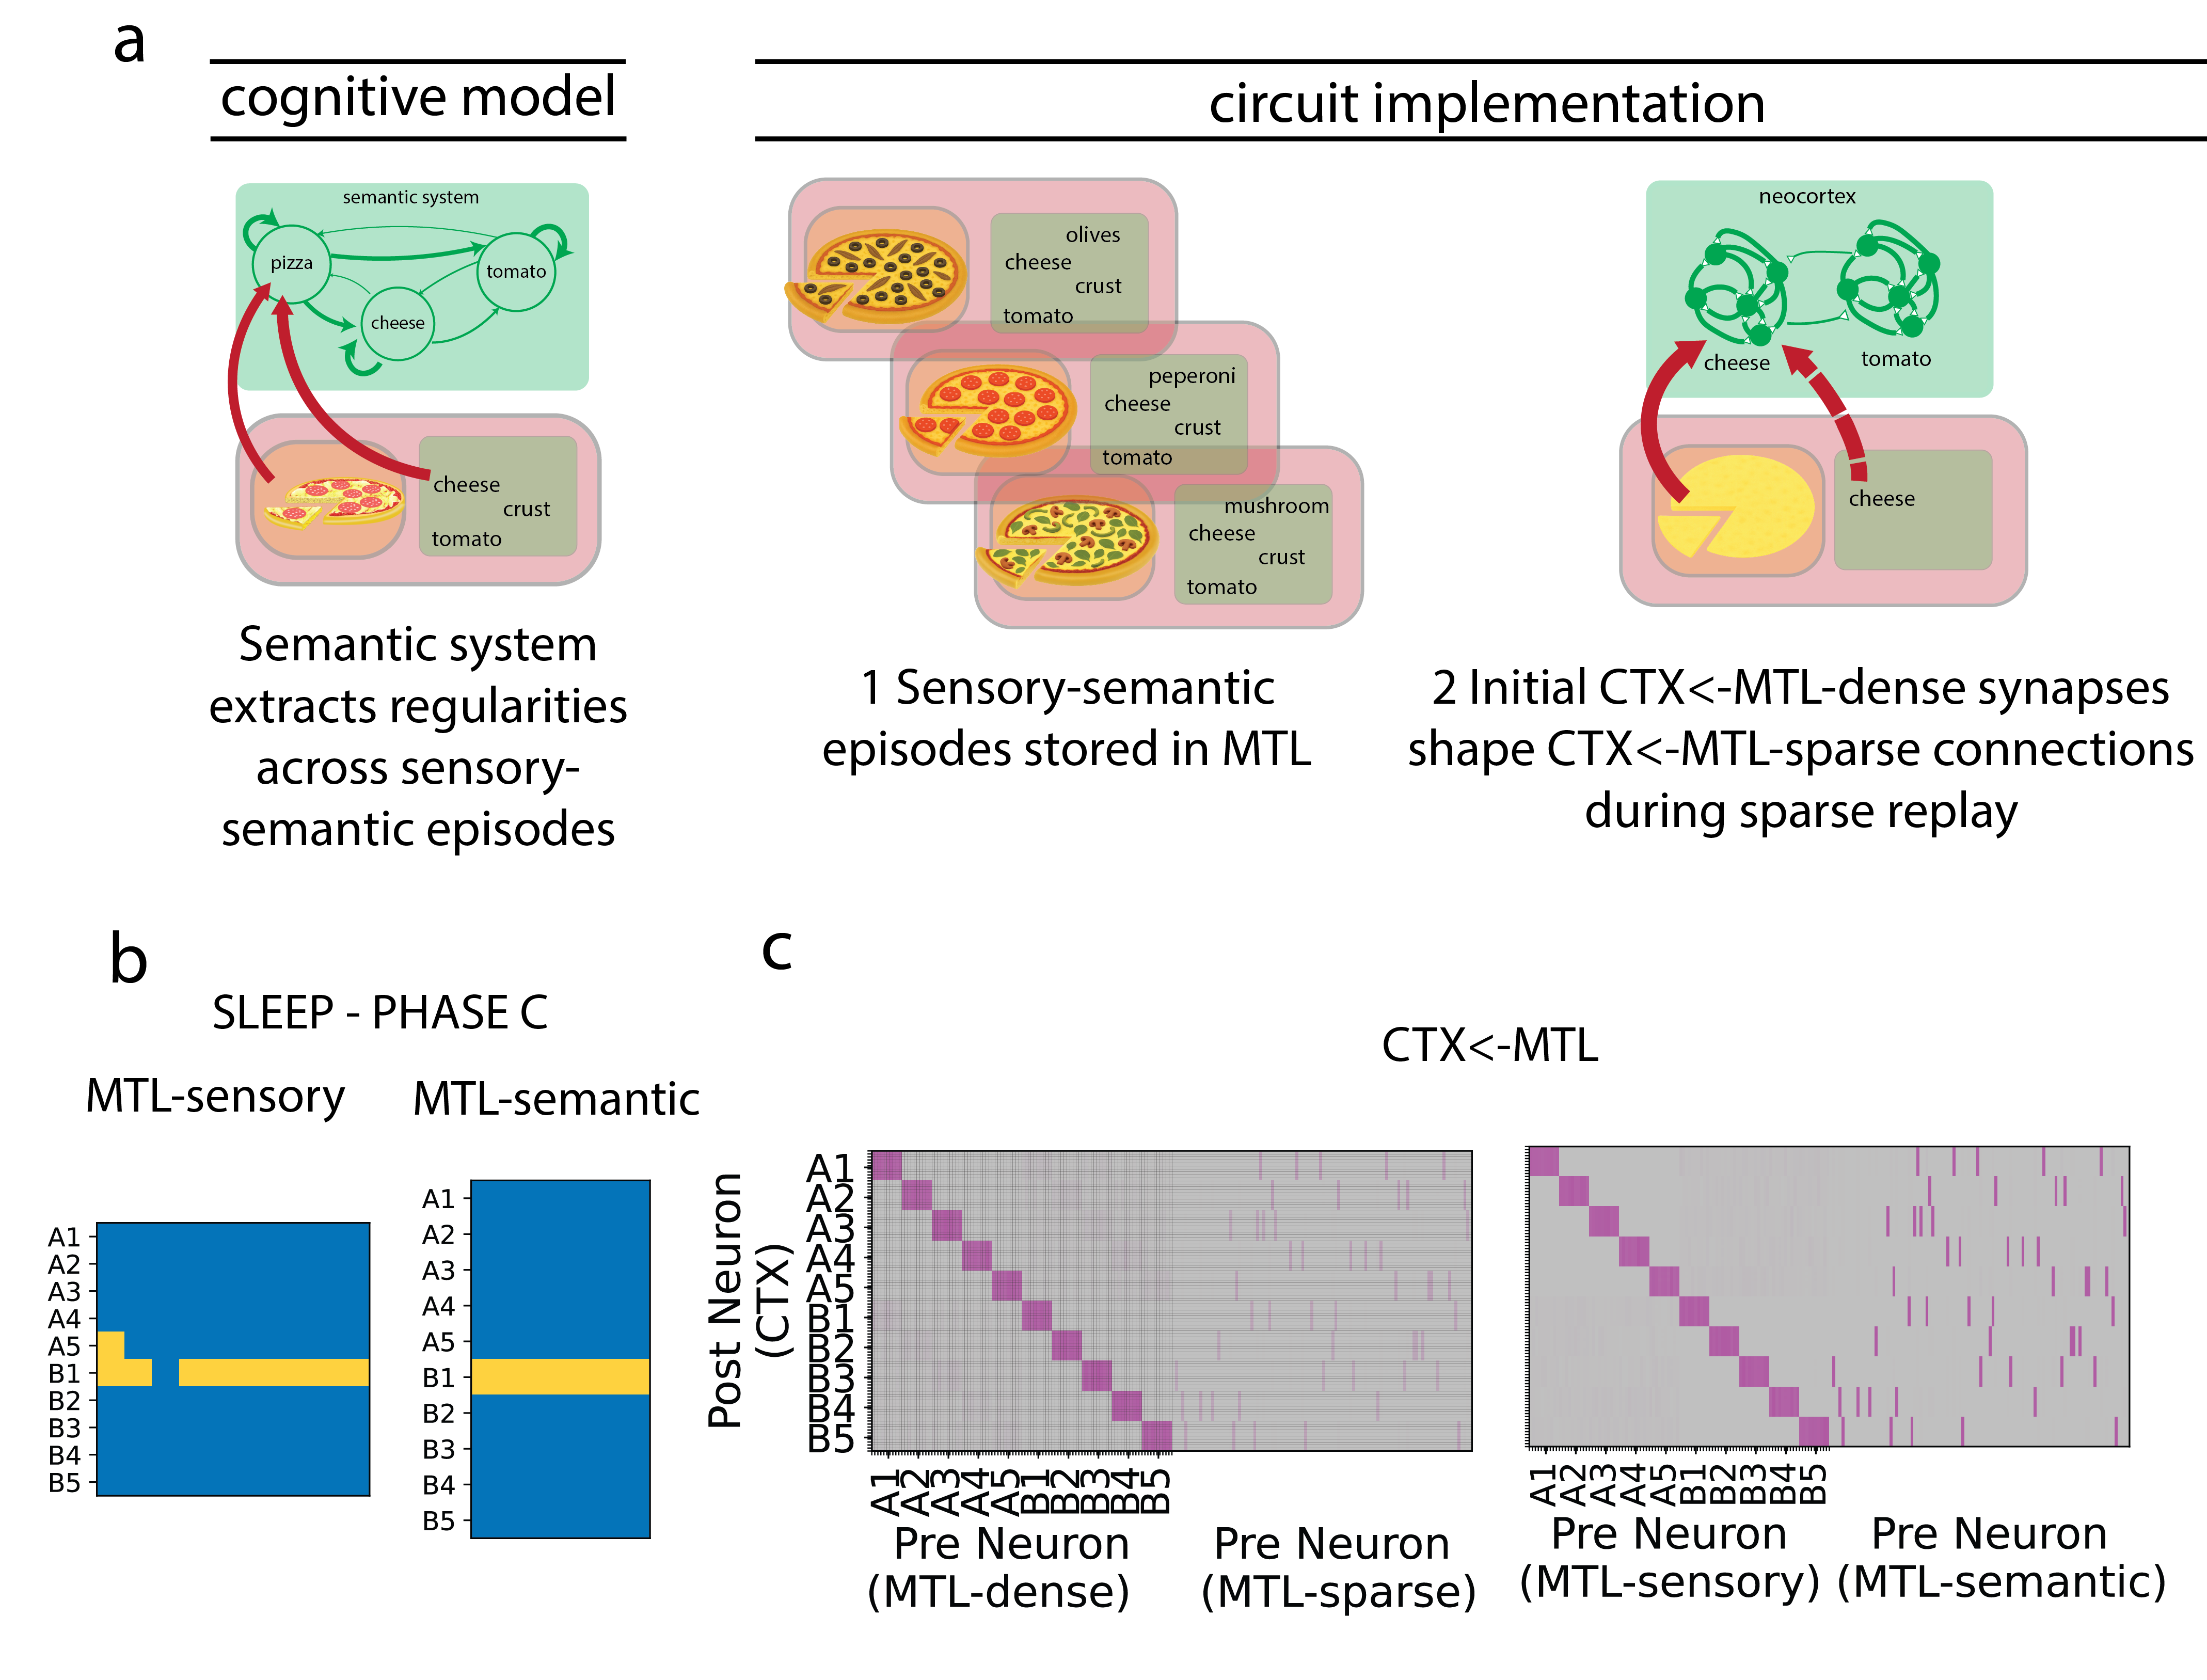
\includegraphics[width=\linewidth]{Figures/Figure_4.png}
    \caption{Caption}
    \label{fig:phase_c}
\end{figure}
\end{comment}
\section*{Discussion}
In this study, we introduce a cognitive strategy by which episodic memory is improved through leveraging previously extracted semantic representations. Our model posits that, following an episodic-to-semantic consolidation process, semantic-to-episodic memory transfer reshapes the code of episodic memory itself. We further propose a biologically plausible neural circuit that implements such cognitive model, successfully capturing the associated learning algorithm. Our circuit model aligns with and explains experimental data, and highlights the behavioural advantages of such a bidirectional learning mechanism.
\newline\newline
First, we demonstrated how episodic replay from hippocampal and para-hippocampal (medial temporal lobe, MTL) regions effectively supports semantic consolidation in cortical (CTX) networks. While this initial step of consolidation corresponds to the most widely studied phase of learning across subcortical-cortical interactions \shortcite{alvarez_1994, mcclelland_1995, oreilly_2014, sun_2023, guerreiro_2024, spens_2024} (to name just a few), our model exhibits key differences from previous models. To start, most models assume a faithful replay of awake subcortical and cortical activity, with abstraction happening directly in CTC$\leftarrow$CTX (neocortex to neocortex) connections. This is problematic for two reasons: first, the assumption that subcortical replay can reinstantate perfectly previous cortical activity is not given \shortcite{swanson_2020}. Secondly, this relies on meaningful (to some degree) representations already existing in neocortex, when it is precisely via semantic consolidation that these representations should be created in the first place. For example, in \shortciteA{chrysanthidis_2022}, semantics are also extracted by forming block-like structure of recurrently connected neurons, but the high specificity of these neurons is already given. Furthermore, many studies assume a copy-paste mechanism between cortex and hippocampus, either directly via one-to-one connections \shortcite{alvarez_1994, tome_2022, guerreiro_2024, spens_2024} or perfect pattern-separating random connections \shortcite{sun_2023}, with less emphasis placed on how synapses mapping one to the other can be formed with biologically plausible learning mechanisms (although previous effort has been made in the context of backpropagation-like error-driven learning rules \shortcite{singh_2022}). In contrast, here we have proposed that increasing sparsity levels during replay can lead to CTX$\leftarrow$MTL synapses becoming selective to frequent episodic sub-patterns. This effectively decorrelates the training input provided to these connections, which could otherwise lead to representational collapse using standard hebbian mechanisms. 
\newline\newline
Next, we proposed a mechanism whereby the semantic structure imprinted in CTX$\leftarrow$CTX connections can be transferred into the coding scheme of MTL. Both the notion that semantics are extracted in CTX \shortcite{mcclelland_1995} and that the MTL encodes a latent representation of the environment \shortcite{quiroga_2005, aronov_2017, behrens_2018} have been present in the literature for a long time, but a mechanistic account of how these representations emerge in MTL remains unknown. We put forward the hypothesis that, after extracted in CTX, spontaneous cortical activity could transfer information encoded in cortical synapses to MTL$\leftarrow$CTX synapses, inducing a semantic code in MTL. We called this process semantic-to-episodic consolidation, and conceptualized it as a mirror of episodic-to-semantic consolidation. As such, instead of transferring episodic information contained in recurrent MTL connections to CTX representations, it transfers semantic information present in recurrent CTX connections to MTL representations. The idea that cortex-to-hippocampus teaching is an underexplored topic in complementary learning systems literature was recently highlighted in \shortciteA{liu_2024}, and implicitly explored in \shortciteA{spens_2024}. In the latter study, the authors explored the possibility of using a Hopfield network to store pairs of sensory-latent representations for episodic recall, in a similar manner that our MTL-sensory and MTL-semantic neurons form joint attractors in MTL recurrent connections. Again, however, the process by which these joint representations were formed was not fully specified, with the model instead employing a copy-paste strategy to generate them. A model that also studied the formation of joint sensory-semantic representations as attractors in hippocampus is the Tolman Eichenbaum Machine \shortcite{whittington_2020}. In this study, the information in the sensory input was already highly semantized (i.e. using a one-hot encoding of sensory features), and the abstract graph position of the stimuli also given a priori. The mechanism for obtaining these representations in the first place was also not explored. In addition to establishing a mechanism for concept cell formation in MTL, our results show that this form of representations is more suitable for rapid learning than mixed representations, both in In-Distribution and Compositional Out-Of-Distribution environmental statistics. This allows MTL to compositionally encode never-seen episodes as long as these correspond to rearrangements of previously seen semantic representations. This is in agreement to previous results in continual learning in artificial neural networks \shortcite{chaudhry_2020}. We also showed how maintaining sensory low-level representations of the environment is crucial for encoding episodes that are Semantic Out-Of-Distribution (that is, when new episodes cannot be encoded using previous semantic representations). 
\newline\newline
Our model has shown how even in non-trivial, highly overlapping scenarios like a random projection of the original input one can obtain concept cells in MTL. Moreover, the model offers a mechanism via which the formation of these representations is favored by blocked (as opposed to interleaved) learning, as demonstrated in humans \shortcite{flesch_2018}. In our model, blocked learning provides the MTL with many different examples of episodes containing the same concept, which are averaged out in its recurrent connections, facilitating the replay of its corresponding prototypical representation \shortcite{posner_1968}. The model also explains why recall of episodes with a higher semantic component is better than that of episodes that, from the perspective of the learned semantic structure, appear random \shortcite{lin_2021}. In classic models of recall based on attractor models, overlaps between episodes is seen as detrimental, reducing the network capacity \shortcite{hopfield_1982, treves_1994}. However, semantic representations have a structured overlap, where the overlap is not stochastic but instead corresponds to the two episodes containing semantic overlaps. Thus, rather than reducing recall, this overlap acts as an error-correcting code \shortcite{albesagonzalez_2025}. Moreover, semantic representations not only show better recall, but also actively improve the recall of the sensory component. Similarly, semantic representations induce replaying activity patterns that resemble more activity during wakefulness. These results can help explain why learning schema-congruent information is much faster than that of completely new episodes \shortcite{tse_2007}. While many models have focused on explaining how faster neocortical learning could happen at the cortex level \shortcite{mcclelland_2013, guerreiro_2024}, our results suggest that this could be in part because the replayed activity in the first place is less noisy. Understanding the mechanisms of positive transfer learning is one of the cornerstones of modern artificial intelligence, where inducing models to use previously learned information to learn new tasks is still a challenge \shortcite{iman_2023}.
\newline\newline
Following this potential link between replay involving semantic representations and continual learning, we showed that closing the loop (performing episodic-to-semantic consolidation of episodes that contain both sensory and semantic representations) allows the formation of higher-order compositional representations in CTX \shortcite{kurth_2023}, in turn inducing a complete semantic description of the causal links across concepts in different levels of abstraction \shortcite{barlow_1972}. Not only higher-order representations (for example pizza is a conjunction of the different ingredients it contains) were developed, but CTX$\leftarrow$CTX connections captured the semantic relationships across these different hierarchical levels (like the fact that pizza is much more related to cheese than cheese is to pizza). Crucially, these forms of asymmetric relationships cannot be captured by classic models of hebbian learning, as recently shown in \shortciteA{albesagonzalez_2025}. YOU HAVE A COMMENT "SUCH AS" IN THE PREVIOUS SENTENCE, COULD YOU CLARIFY. Finally, these results open the door to a mechanism for \textit{infantile amnesia}. Our model predicts that consolidating in CTX memories of higher semantic load (such as full episodes, which consist in the association of multiple concepts) is easier in the presence of previous semantic representations. In this context, one interpretation of infantile amnesia could be the following: during early development infants create an initial repertoire of simple concepts, but replay of full episodes is hindered by the absence of initial semantic structure in MTL. With time, simple conceptual representations emerge in MTL, allowing the consolidation of concepts of higher complexity, which are more episodic-like. For example, after many months forming conceptual representations related to family members or house locations, an infant would be able to consolidate an episode involving particular combinations of these, while before only compositional structure across episodes could be extracted.
\newline\newline
The model faces several limitations at different levels. In a sense, the model is positioned in an opposite end in the perfectly-pattern-separated vs perfectly-overlapping spectrum of hippocampal representations. While this has shown several advantages, we know that structures like the dentate gyrus act as a pattern separator, inducing changes in representations even across similar episodes, as recently evidenced by episode-specific coding neurons in \shortcite{kolibius_2023, chettih_2024}. At the same time, some representations are shared across different episodes, as evidenced by place cells and concept cells, when episodes have correlated environmental variables. Further studies using a combination of shared and non-shared neuronal subspaces across similar episodes could explore a combination of both strategies could facilitate learning and optimal behaviour (efforts in this direction have been made before \shortcite{schapiro_2017}). While we have slightly moved away from completely orthogonal input representations usually used in biologically-plausible mechanistic models of consolidation, the input used here was still relatively simple, with more complex representations still requiring gradient-based methods. How the brain might use local plasticity rules to learn from more realistic input remains an open question. Another computational limitation of the model resides in the over-simplicity of the different regions, studying CTX and MTL as single recurrent layers. While this is a standard practice in models of consolidation, future work could explore how similar mechanisms to the ones proposed here can learn using hierarchical cortical and subcortcial circuits.
\newline\newline
The results presented here could finally be of significance for modern artificial neural networks. In the recent years, many authors have highlighted episodic memory as a missing piece in many Artificial Intelligence paradigms \shortcite{fountas_2025, dong_2025, pink_2025}.  Our model suggests that episodic memory should not simply be added as a fast external buffer, but rather be continuously reshaped by semantic knowledge. This bidirectional interaction yields three advantages directly relevant for AI: (i) more robust recall of past experiences through semantic “error correction,” and (ii) the ability to rapidly learn new combinations of previously known concepts, supporting compositional generalization. Such designs may allow modern neural networks to leverage prior structure in order to accelerate continual learning and adapt flexibly to new environments.
\newpage
\section*{Methods}\label{methods}

\subsection*{Circuit Model}
\subsubsection*{Architecture and nomenclature}
\paragraph*{Regions and neural activity}
We study a sparse, subregional network with regions $R \in \{\text{hidden},\, \text{output}\}$. Each region $R$ is partitioned into $K_R$ subregions of sizes $|S_{R,1}|,\dots,|S_{R,K_R}|$ with total size $|S_R|=\sum_k |S_{R,k}|$. Neural activity is binary and sparse. We denote activity by $X$, with $X^R \in \{0,1\}^{|S_R|}$, and pre-activation by $\hat{X}^R$. The $i$-th neuron in region $R$ is $X^R_i$. Region-specific sparsity parameters control the fraction of active units per subregion during wake and sleep ($\rho_R$ and $\rho_R^{\text{sleep}}$).

Each region maintains two auxiliary vectors: an immaturity mask $\mathrm{IM}^R \in \{0,1\}^{|S_R|}$ and an excitability vector $b^R \in \mathbb{R}^{|S_R|}$. These are initialized from configuration: $\mathrm{IM}^R_i=1$ for immature regions and $0$ otherwise; $b^R_i = \beta_R$ for all $i$.

\paragraph*{Connectivity}
Directed synaptic matrices connect $\textrm{pre}\to\textrm{post}$ regions as $W^{\textrm{post}\leftarrow\textrm{pre}} \in \mathbb{R}^{|S_{\textrm{post}}|\times|S_{\textrm{pre}}|}$. A synapse from $j$ in pre to $i$ in post is $W^{\textrm{post}\leftarrow\textrm{pre}}_{ij}$. In the minimal configuration used here, we instantiate two connections: $\text{hidden}\leftarrow\text{hidden}$ (recurrent) and $\text{output}\leftarrow\text{hidden}$ (feed-forward). Connections may be declared frozen (non-plastic) or learn online via local Hebbian updates (see Plasticity).

\subsubsection*{Synaptic initialization}
We initialize connectivity following a receptive-field (RF) random scheme with optional Gaussian jitter. For $W^{\textrm{post}\leftarrow\textrm{pre}}$, we select $k$ indices per \emph{post} (or per \emph{pre}) uniformly at random and set equal non-zero weights so that either
\begin{itemize}
  \item per-post sums equal $W^{\textrm{post}\leftarrow\textrm{pre}}_{\text{max-post}}$ (mode \emph{post}), or
  \item per-pre sums equal $W^{\textrm{post}\leftarrow\textrm{pre}}_{\text{max-pre}}$ (mode \emph{pre}).
\end{itemize}
Finally, i.i.d. Gaussian noise $\mathcal{N}(0,\sigma^2)$ can be added. For mode \emph{post}: for each $i$ (post unit), sample $S_i \subseteq \{1,\dots,|S_{\textrm{pre}}|\}$ with $|S_i|=k$ and set $W^{\textrm{post}\leftarrow\textrm{pre}}_{i,S_i} = W^{\textrm{post}\leftarrow\textrm{pre}}_{\text{max-post}}/k$ (0 elsewhere), then add noise. This scheme is used for $\text{hidden}\leftarrow\text{hidden}$ and $\text{output}\leftarrow\text{hidden}$ with RF sizes and caps specified in the parameter dictionary.

\subsection*{Network Operations}
\subsubsection*{Neuronal activation}
Within each subregion $S_{R,k}$, the operator $\mathcal{A}$ selects the top $K=\lfloor\rho_{R,k}\,|S_{R,k}|\rfloor$ entries of $\hat{X}^R[S_{R,k}]$ and sets them to 1 (others to 0). A small noise term is added to $\hat{X}$ to break ties deterministically. During sleep, if a subregion index is specified (or chosen by total drive), only that subregion is activated at the given sparsity.

\subsubsection*{Feed-forward input processing}
At wake timestep $t$, the minimal forward used in our figures computes
\begin{equation}
    X^{\text{hidden}} \leftarrow \mathcal{A}(x_t),\qquad
    \hat{X}^{\text{output}} \leftarrow W^{\text{output}\leftarrow\text{hidden}}\,X^{\text{hidden}},\qquad
    X^{\text{output}} \leftarrow \mathcal{A}(\hat{X}^{\text{output}}),
\end{equation}
with $x_t$ the external drive. Recurrent pattern completion (optional) updates a recurrent region $R$ by iterating
\begin{equation}
    X^{R}_{k+1} \leftarrow \mathcal{A}\bigl(W^{R\leftarrow R}\,X^{R}_{k}\bigr)
\end{equation}
for a fixed number of steps $k$.

\subsubsection*{Pattern completion (recurrent input processing)}
Given a recurrent matrix $W^{R\leftarrow R}$, pattern completion is an iterative update on $X^{R}$ initiated at $X^{R}_0$ for a fixed number of iterations. It is used for attractor-like retrieval and for generating structured sleep cues when desired.

\subsection*{Plasticity}
\subsubsection*{Hebbian Learning}
Synapses update by a local outer-product rule:
\begin{equation}
            \Delta W^{\textrm{post} \leftarrow \textrm{pre}} = \lambda^{\textrm{post} \leftarrow \textrm{pre}}\, X^{\textrm{post}} (X^{\textrm{pre}})^\top,\qquad
            W^{\textrm{post} \leftarrow \textrm{pre}} \leftarrow W^{\textrm{post} \leftarrow \textrm{pre}} + \Delta W^{\textrm{post} \leftarrow \textrm{pre}}.
\end{equation}
Connections can be frozen (no learning). In the minimal awake pass we update $\text{hidden}\leftarrow\text{hidden}$ each step; other connections can be included as configured.

\subsubsection*{Homeostatic Plasticity}
To prevent runaway growth and enforce synaptic competition, we apply multiplicative normalizations that cap total outgoing and incoming strengths whenever finite caps are provided. For rows (post):
\begin{equation}
    \text{if }\sum_j W_{ij} > W^{\textrm{post}\leftarrow\textrm{pre}}_{\text{max-post}}\;\Rightarrow\; W_{i,:} \leftarrow W_{i,:}\,\frac{W^{\textrm{post}\leftarrow\textrm{pre}}_{\text{max-post}}}{\sum_j W_{ij}}.
\end{equation}
For columns (pre):
\begin{equation}
    \text{if }\sum_i W_{ij} > W^{\textrm{post}\leftarrow\textrm{pre}}_{\text{max-pre}}\;\Rightarrow\; W_{:,j} \leftarrow W_{:,j}\,\frac{W^{\textrm{post}\leftarrow\textrm{pre}}_{\text{max-pre}}}{\sum_i W_{ij}}.
\end{equation}
If a cap is omitted or $\infty$, the corresponding normalization is skipped.

\subsection*{Initialization}
\subsubsection*{Region and subregion specification}
We specify the set of regions $\mathcal{R}=\{\text{hidden},\,\text{output}\}$. For each region $R$ we set: (i) number of subregions $K_R$ and sizes $(|S_{R,1}|,\dots,|S_{R,K_R}|)$, (ii) sparsity vectors $\rho_R$ (wake) and $\rho_R^{\text{sleep}}$ (sleep), and (iii) immaturity and excitability: $\mathrm{IM}^R_i=1$ iff $R$ is configured immature, 0 otherwise; $b^R_i=\beta_R$ for all $i$.

\subsubsection*{Connectivity parameters}
For each $W^{\textrm{post}\leftarrow\textrm{pre}}$ to instantiate we provide: init type $\in\{\text{zero},\,\text{random}\}$, RF mode $\in\{\text{post},\,\text{pre}\}$, RF size $k$, init std $\sigma$, caps $W^{\textrm{post}\leftarrow\textrm{pre}}_{\text{max-post}}$, $W^{\textrm{post}\leftarrow\textrm{pre}}_{\text{max-pre}}$, learning rate $\lambda^{\textrm{post}\leftarrow\textrm{pre}}$, and optional freeze flags.

\subsection*{Input Generation}
\subsubsection*{Compositional latent space}
Inputs are generated from a factorized latent space with $L$ factors (e.g., two factors $A$ and $B$). A latent label $\ell=(\ell_1,\dots,\ell_L)$ selects a block of active units per factor; the full binary pattern concatenates across factors. Episodes are piecewise-constant segments of duration $D$ (fixed or Poisson with mean $\mu$). We inject corruption via \emph{swap} noise: at each step a specified number of on$\to$off and off$\to$on flips are applied either globally or proportionally within specified regions. The generator yields tensors of shape $(\text{num\_days},\,\text{day\_length},\,\text{input\_dim})$, integer episode indices, and per-factor latent labels.

\subsection*{Training Protocol}
\subsubsection*{Awake phase}
For each day, we iterate over timesteps, compute the forward pass, apply Hebbian updates to enabled connections, apply homeostatic caps, and record activities/connectivity at configured rates.

\subsubsection*{Sleep phase (optional)}
After wake, an optional sleep routine runs for $T_{\text{sleep}}$ steps, invoking a replay primitive (e.g., $\text{hidden}\to\text{output}$) and recording sleep indices. In the minimal placeholder used here, replay is generic and does not alter connectivity unless a learning rule is bound for those connections.

\subsection*{Recording and Analysis}
\subsubsection*{Recording}
We track selected region activities and connectivity matrices based on user-specified lists and rates. We maintain global time indices and separate awake and sleep index lists to align analyses with recorded tensors.

\subsubsection*{Selectivity and accuracy}
Neuron–latent selectivity is computed as correlation between normalized activity and latent indicators. For decoding accuracy, each neuron is assigned to its argmax latent; per-timestep predicted latent is the argmax over counts of active neurons supporting each latent. We report mean accuracy per latent. We also build ordered assemblies by selecting top-selective neurons per latent with backfilling from a discard pool if needed.

\subsection*{Hyperparameters}
Unless stated otherwise, representative values are: (i) Regions and sparsity: hidden with $K=1$–$2$ subregions of sizes $50$–$100$ and $\rho\approx0.1$–$0.2$ (wake/sleep), output size $50$ with $\rho\approx0.04$; (ii) recurrent completion: $10$ iterations where used; (iii) Hebbian and caps: $\lambda^{\text{hidden}\leftarrow\text{hidden}}\approx5\cdot10^{-4}$ with $W^{\text{hidden}\leftarrow\text{hidden}}_{\text{max-post}}=\infty$, $W^{\text{hidden}\leftarrow\text{hidden}}_{\text{max-pre}}=1$; $\lambda^{\text{output}\leftarrow\text{hidden}}\approx5\cdot10^{-4}$ with $W^{\text{output}\leftarrow\text{hidden}}_{\text{max-post}}=1$, $W^{\text{output}\leftarrow\text{hidden}}_{\text{max-pre}}=\infty$; (iv) initialization: random RFs with sizes $30$ (hidden$\leftarrow$hidden) and $10$ (output$\leftarrow$hidden), small Gaussian jitter ($\sigma\approx5\cdot10^{-4}$); (v) inputs: day length $40$–$25\,000$, mean duration $\mu=5$ (fixed or Poisson), swap noise of 4 flips per step; two-factor latent spaces such as $5\times10$.

\subsection*{Implementation and Reproducibility}
The model is implemented in PyTorch with explicit tensor updates (no autograd required). Seeds for Python, NumPy, and Torch are set where indicated. Code structure: network scaffold and utilities (\texttt{src/model.py}), parameterization and experiment hooks (\texttt{Network\_Definition/parameters.py}, \texttt{forward.py}, \texttt{sleep.py}), input and analysis tools (\texttt{src/utils/general.py}, \texttt{src/utils/Figure\_2.py}). All figures are generated from notebooks in the repository.

% --- Hide previous Methods (kept for reference) ---
\begin{comment}
\subsection*{Circuit Model}
\subsubsection*{Architecture and nomenclature}
\paragraph*{Regions and neural activity}
The circuit model contains 3 main regions: sensory cortex (SEN), neocortex (CTX), and medial temporal lobe (MTL). In turn, MTL is split into two sub-regions: MTL-sensory and MTL-semantic. We use $X$ to denote the neural activity, which is written as $X^\textrm{region}$ (for example $X^\textrm{CTX}$) when the region is to be made explicit. The same follows for pre-activation (synaptic) input, which is denoted by $\hat{X}$ (or $\hat{X}^\textrm{region})$. The activity of neuron $i$ in a region is $X^\textrm{region}_i$. The number of neurons in a region is denoted by $N_\textrm{region}$ (e.g. $N_\textrm{CTX}$).
\paragraph{Connectivity}
Connectivity matrices connecting a region \textrm{pre} to a region \textrm{post} take the form $W^{\textrm{post}\leftarrow\textrm{pre}}$, and a synapse connecting neuron $j$ in region pre with neuron $i$ in region post is $W^{\textrm{post}\leftarrow\textrm{pre}}_{ij}$. For example, $W^{\textrm{CTX}\leftarrow\textrm{MTL}}_{13}$ represents the connection of neuron 3 in MTL with neuron 1 in CTX. Connectivity is classified as either feed-forward (connecting two different regions), which includes  $W^{\textrm{MTL-sensory}\leftarrow\textrm{SEN}}$, $W^{\textrm{CTX}\leftarrow\textrm{MTL}}$, and $W^{\textrm{MTL-semantic}\leftarrow\textrm{CTX}}$, and recurrent (connecting a region with itself), which includes $W^{\textrm{CTX}\leftarrow\textrm{CTX}}$, and $W^{\textrm{MTL}\leftarrow\textrm{MTL}}$. All connections are plastic except $W^{\textrm{MTL-sensory}\leftarrow\textrm{SEN}}$, which is fixed. Given a connectivity matrix $W^{\textrm{post}\leftarrow\textrm{pre}}$, we call receptive field of a postsynaptic neuron $i$ $\textrm{RF}^{\textrm{post}\leftarrow\textrm{pre}}_i$ the vector representing the connections from region pre to postsynaptic neuron $i$
\begin{equation}
    \textrm{RF}^{\textrm{post}\leftarrow\textrm{pre}}_i = \{{W^{\textrm{post}\leftarrow\textrm{pre}}}_{kj}\} \;\; : \;k = i 
\end{equation}
\paragraph{Synaptic Initialization}
\paragraph{Sensory cortex to MTL-sensory}
In Figs. \ref{fig:phase_a} and \ref{fig:phase_b}, $W^{\textrm{MTL-sensory}\leftarrow\textrm{SEN}}$ is initialized as the identity, mapping to MTL-sensory an exact copy of $X^\textrm{SEN}$. In the rest of Figures, the matrix is generated randomly with the condition that all receptive fields are of equal size.
\begin{equation}
    || RF_i ||_0 = |\{j \in \{1, ..., N_\textrm{SEN}\} : W^{\textrm{MTL-sensory}\leftarrow\textrm{SEN}}_{ij} \neq 0\}| = W^{\textrm{MTL-sensory}\leftarrow\textrm{SEN}}_\textrm{size}\;\; \forall i
\end{equation}
and sum:
\begin{equation}
    \sum_j\{RF_i^{\textrm{MTL-sensory}\leftarrow\textrm{SEN}}\}_j = \sum_jW^{\textrm{MTL-sensory}\leftarrow\textrm{SEN}}_{ij} = W^{\textrm{MTL-sensory}\leftarrow\textrm{SEN}}_\textrm{max-in}\;\; \forall i
\end{equation}
where $|| RF_i ||_0$ denotes the $l_0$ norm (which counts the number of non-zero entries), $W^{\textrm{MTL-sensory}\leftarrow\textrm{SEN}}_\textrm{size}$ is a network parameter determining the number of non-zero connections each receptive field has, and $W^{\textrm{MTL-sensory}\leftarrow\textrm{SEN}}_\textrm{max-in}$ another network parameter determining the maximum sum of incoming connections a postsynaptic neuron has. In order to achieve both conditions, we generate $W^{\textrm{MTL-sensory}\leftarrow\textrm{SEN}}$ by randomly sampling each receptive field $i$ independently, following:
\begin{equation}
    \{RF_i\}_j =
\begin{cases}
\frac{W^{\textrm{MTL-sensory}\leftarrow\textrm{SEN}}_\textrm{max-in}}{W^{\textrm{MTL-sensory}\leftarrow\textrm{SEN}}_\textrm{size}}, & \text{if } j \in S, \\
0, & \text{if } j \notin S,
\end{cases}
\end{equation}
with $S$ a random subset of the presynaptic entries:
\begin{equation} 
S \sim \text{Unif}\big\{ T \subseteq \{1,\dots,N_\textrm{SEN}\} : |T| = W^{\textrm{MTL-sensory}\leftarrow\textrm{SEN}}_\textrm{size} \big\} \Longrightarrow  |S| = W^{\textrm{MTL-sensory}\leftarrow\textrm{SEN}}_\textrm{size}, 
\end{equation}
where $|A|$ denotes the number of elements in set $A$.
\paragraph{Feed-Forward connections}
Feed-forward connections are sampled from a Gaussian distribution with mean 0 and standard deviation $W^{\textrm{post}\leftarrow\textrm{pre}}_\sigma$ as a network parameter.
\begin{equation}
    W^{\textrm{post}\leftarrow\textrm{pre}}_{ij} \sim \mathcal{N}(0, W^{\textrm{post}\leftarrow\textrm{pre}}_\sigma)
\end{equation}
\paragraph{Recurrent connections}
Recurrent connections are initialized at 0. MTL connections are reset every \textit{day} (see Algorithm \ref{alg:train})
\paragraph{Mature and immature neurons} Neurons in the model can be either \textit{mature} or \textit{immature}. The intuition is: do these neurons contain meaningful representations via input received from another region (mature) or are mostly non-selective and random (immature)? More details on the dynamics and plasticity of mature and immature neurons can be seen below, but to summarize: (i) immature neurons have higher excitability during feed-forward input processing and (ii) immature neurons have a higher learning rate in its incoming feed-forward connections and its recurrent connections frozen. The intuition is that by having higher excitability, during receptive field formation in feed-forward synapses, immature neurons win the competition for postsynaptic activity only if the presynaptic pattern is too far from the receptive fields that have already formed. By doing this, if a presynaptic pattern is similar to previously formed representations, it slightly changes the already formed representations. If not, a set of immature neurons win the competition, develop receptive field due to higher plasticity, and then become mature. This allows one-shot formation of new postsynaptic representations of presynaptic input when an input pattern is too different from those presented to the network before, and then refining these representations with a slower learning rate. Similarly, recurrent connectivity, which reflects statistical regularities across the representations formed, is only developed between mature neurons that actually code for an environmental variable, to avoid recurrent connections representing spurious correlations. Maturity in a region is denoted by $\textrm{IM}^\textrm{region}$, where $\textrm{IM}^\textrm{region}_i = 1$ if neuron $i$ in the region is immature, and 0 otherwise.
\subsection*{Network Operations}
\subsubsection*{Neuronal activation}
Synaptic input is mapped to neural activity via a \textit{K-winners-share-all} mechanism, in which the $K$ neurons with the highest pre-activation input $\hat{X}$ set their activity to 1, and the rest to 0. This can be written as
\begin{equation}
    X = \textrm{top-}K\big(\hat{X}\big)
\end{equation}
In  order to determine $K$ in a particular region, first we define
\begin{equation}
    K^\textrm{region}_\textrm{concept} \leq K^\textrm{region}_\textrm{episode}
\end{equation}
 such that each concept is represented by $K^\textrm{region}_\textrm{concept}$ neurons, and a typical episode during wakefulness contains $K^\textrm{region}_\textrm{episode}$ active neurons. In this context, given $K$ active neurons in a region, we define the semantic load $S_L$ to be the number of concepts represented by $K$ neurons, such that
 \begin{equation}
     K = S_L \cdot K^\textrm{region}_\textrm{concept}
     \label{eq:semantic_load}
 \end{equation}
In other words, by fixing the semantic load, one fixes how many neurons in total are active, making $K$ higher if more concepts are being represented. The maximum number of concepts that can be encoded in an episode is thus:
 \begin{equation}
     N^\textrm{region}_\textrm{concept} = \frac{K^\textrm{region}_\textrm{episode}}{K^\textrm{region}_\textrm{concept}}
 \end{equation}
 Therefore, we can define \textsc{Activate} (Algorithm \ref{alg:activate}) as an algorithm that maps presynaptic input $\hat{X}$, given a semantic load $S_L$, into neural activation $X$ in the following way:
\begin{algorithm}[h!]
\caption{Neuronal Activation}\label{alg:activate}
\begin{algorithmic}[1]
\Function{Activate}{$\hat{X}$, $\textrm{region}$, $S_L$}
    \State Compute number of active neurons:
        \[
            K \gets S_L \times K^\textrm{region}_\textrm{concept}
        \]
    \State Select top-$K$ entries:
        \[
            X \gets \textrm{top-}K(\hat{X})
        \]
    \State \Return $X$
\EndFunction
\end{algorithmic}
\end{algorithm}

\subsubsection*{Feed-forward input processing}
Input processing is computed for a single pre and post region at a time, with pre-activation input $\hat{X}^\textrm{post}$ obtained via
\begin{equation}
    \hat{X}^\textrm{post} = W^{\textrm{post}\leftarrow\textrm{pre}} \cdot X^\textrm{pre} + b^\textrm{post}\textrm{IM}^\textrm{post}
\end{equation}
$b^\textrm{post}$ is the extra excitability that immature neurons have in region post.
\subsubsection*{Pattern completion (recurrent input processing)}
Given a recurrent network, pattern completion is typically defined as an iterative update on neural activity $X^\textrm{region}$ that is initiated in an initial state $X^\textrm{region}_0$:
\begin{equation}
    X^{\textrm{region}}_{k+1} = \textrm{top-}K(W^{\textrm{region}\leftarrow\textrm{region}}\cdot X^\textrm{region}_{k})
\end{equation}
with $W^{\textrm{region}\leftarrow\textrm{region}}$ the region recurrent connectivity matrix, $K$ dependent on the specified semantic load $S_L$, and $k$ a timestep operating on a smaller timescale,  than the overall timescale $t$. This means that within a timestep $t$, there are pattern\_complete\_iterations iterations on temporal index $k$. This is used to define \textsc{PatternComplete}  as Algorithm \ref{alg:pattern_complete}:
\begin{algorithm}[h!]
\caption{Pattern Completion}\label{alg:pattern_complete}
\begin{algorithmic}[1]
\Function{PatternComplete}{$X_0$, $S_L$,   \texttt{pattern\_complete\_iterations}}
    \State $X \gets X_0$
    \For{$\text{iteration} = 1$ to $\texttt{pattern\_complete\_iterations}$}
        \State $\hat{X} \gets W^{\textrm{region} \leftarrow \textrm{region}} \cdot X$
    \State $X \gets \textsc{Activate}\bigl(\hat{X}, \textrm{region}, S_L \bigr)$
    \EndFor
    \State \Return $X$
\EndFunction
\end{algorithmic}
\end{algorithm}
\subsubsection*{Hebbian Learning}
The connection between a presynaptic neuron $j$ and a postsynaptic neuron $i$ subject to Hebbian learning is updated as:
\begin{equation}
            \Delta W_{ij} = \lambda_{ij}^{\textrm{post} \leftarrow \textrm{pre}}
            X_i^\textrm{post} X_j^\textrm{pre}
\end{equation}
for a presynaptic region pre and a postsynaptic region post.
\paragraph*{Maturity-dependent learning rate (feed-forward connections)}
In order to combine one-shot and statistical learning in feed-forward synapses (see \shortciteA{albesagonzalez_2025}), the learning rate of feed-forward (post $\neq$ pre) connections depends on the \textit{maturity} of the postsynaptic neuron, which is given by $\textrm{IM}$. Neurons start in an \textit{immature} state $\textrm{IM}_i = 1$, allowing them to form relatively selective initial receptive fields. Once this initial receptive field is formed, the learning rate is reduced to capture the statistical regularities of the presynaptic patterns driving the postsynaptic neuron (the neuron is \textit{mature}, $\textrm{IM}_i = 0$). To do this, we define a quick learning rate
\begin{equation}
        \lambda^{\textrm{post}\leftarrow\textrm{pre}}_\textrm{quick} = \frac{W^{\textrm{post}\leftarrow\textrm{pre}}_\textrm{max-in}}{K^\textrm{pre}} 
\end{equation}
where again $W^{\textrm{post}\leftarrow\textrm{pre}}_\textrm{max-in}$ is a network parameter determining the maximum sum of incoming connections the matrix $W^{\textrm{post}\leftarrow\textrm{pre}}$ has for every postsynaptic neuron ($\sum_jW^{\textrm{post}\leftarrow\textrm{pre}}_{ij} \leq W^{\textrm{post}\leftarrow\textrm{pre}}_\textrm{max-in}$). Then, at each Hebbian update, we have
\begin{equation}
    \lambda_{ij}^{\textrm{post} \leftarrow \textrm{pre}} = (1 - \textrm{IM}^\textrm{post}_i)\lambda^{\textrm{post} \leftarrow \textrm{pre}}_\textrm{slow} + \textrm{IM}^\textrm{post}_i\lambda^{\textrm{post}\leftarrow\textrm{pre}}_\textrm{quick}
\end{equation}
where $\lambda^{\textrm{post} \leftarrow \textrm{pre}}_\textrm{slow}$ is a network parameter indicating the slow learning rate (used throughout all simulations except for the first receptive field formed at each postsynaptic neuron). Note how for an initial (before maturity) driving presynaptic pattern $X^\textrm{pre}$ this guaranties that the initial receptive field formed is $X^\textrm{pre}$ scaled such that the sum of incoming connections is exactly equal to $W^{\textrm{post}\leftarrow\textrm{pre}}_\textrm{max-in}$, as the $K$-winners-share-all mechanism imposes exactly $K_\textrm{pre}$ active neurons. 
\paragraph*{Maturity-dependent learning rate (recurrent connections)}
Recurrent connections are designed to capture conditional firing probabilities between neurons. When individual neurons become mature and tuned to individual concepts, this allows capturing the environment semantic structure. To avoid capturing the statistical structure of immature neurons, and based on the fact that learning in CTX is favoured by the previous formation of schemas \shortcite{tse_2007}, we follow an opposite recipe. Hebbian updates on recurrent connections are only effective if both pre- and postsynaptic neurons are mature:
\begin{equation}
    \lambda_{ij}^{\textrm{region} \leftarrow \textrm{region}} = (1 - \textrm{IM}^\textrm{post}_i)(1 - \textrm{IM}^\textrm{post}_j)\lambda^{\textrm{region}\leftarrow\textrm{region}}_0
\end{equation}
In the case of recurrent connections, there are no slow and quick learning rates, but the parameter $\lambda^{\textrm{post}\leftarrow\textrm{pre}}_0$ is used to distinguish it from the maturity-dependent learning rate matrix 
\paragraph*{Hebbian learning algorithm}
Altogether, this defines \textsc{Hebbian} (Algorithm \ref{alg:hebbian}) as the following update in $W^{\textrm{post} \leftarrow \textrm{pre}}$:
\begin{algorithm}
\caption{Hebbian Learning}\label{alg:hebbian}
\begin{algorithmic}[1]
\Function{Hebbian}{$\textrm{post}$, $\textrm{pre}$}
    \State Obtain learning rate matrix:
    \If{$\textrm{post} \neq \textrm{pre}$}
    \State
        \[
            \lambda_{ij}^{\textrm{post} \leftarrow \textrm{pre}}
            \gets
            (1-\textrm{IM}^\textrm{post}_i)\,\lambda^{\textrm{post} \leftarrow \textrm{pre}}_\textrm{slow}
            + \textrm{IM}^\textrm{post}_i\,\lambda^{\textrm{post}\leftarrow\textrm{pre}}_{\textrm{quick}}
        \]
    \Else
    \State 
    \[
    \lambda_{ij}^{\textrm{post} \leftarrow \textrm{pre}} \gets (1 - \textrm{IM}^\textrm{post}_i)(1 - \textrm{IM}^\textrm{pre}_j)\lambda^{\textrm{post}\leftarrow\textrm{pre}}_\textrm{0}
    \]
    \EndIf
    \State Compute Hebbian update with activity outer product:
        \[
            \Delta W \gets \lambda^{\textrm{post} \leftarrow \textrm{pre}} \odot 
            \Bigl(X^{\textrm{post}} \otimes X^{\textrm{pre}}\Bigr)
        \]
    \State Update weights:
        \[
            W^{\textrm{pre} \leftarrow \textrm{post}} 
            \gets 
            W^{\textrm{pre} \leftarrow \textrm{post}} + \Delta W
        \]
\EndFunction
\end{algorithmic}
\end{algorithm}
\subsubsection*{Homeostatic Plasticity}
We use multiplicative normalization that guarantees, for every weight matrix $W^{\textrm{post}\leftarrow\textrm{pre}}$, the total sum of incoming or outgoing connections is capped to a certain value. Following \shortciteA{albesagonzalez_2025}, we use \textit{incoming homeostasis} as:
\begin{equation}
W_{ij}^{k+1}=
\begin{cases}
 W_{ij}^{k}\cdot\frac{W_\textrm{max-in}}{\sum_{j}W^{k}_{ij}} & \text{if }\sum_{j}W^{k}_{ij} = W_\textrm{max}^\textrm{in} + \epsilon_i, \;\; \epsilon_i > 0 \\[1.2ex]
W^k_{ij}& \textrm{else}
\end{cases}
\end{equation}
where $W^k_{ij}$ denotes the value of synapse $ij$ before applying homeostasis and $W^{k+1}_{ij}$ the value after applying homeostasis (for readability, we simply write $W \equiv W^{\textrm{post}\leftarrow\textrm{pre}}$).
Similarly, we have \textit{outgoing homeostasis} to be defined by:
\begin{equation}
W_{ij}^{k+1} =
\begin{cases}
 \frac{W_\textrm{max-out}}{\sum_{i}W^k_{ij}} & \text{if }\sum_{j}W^k_{ij} = W_\textrm{max}^\textrm{out} + \epsilon_j, \;\; \epsilon_j > 0 \\[1.2ex]
0 & \textrm{else}
\end{cases}
\end{equation}
This allows, for a presynaptic region pre and a postsynaptic region post, defining \textsc{Homeostasis} (Algorithm \ref{alg:homeostasis}) as:
\begin{algorithm}
\caption{Homeostasis}\label{alg:homeostasis}
\begin{algorithmic}[1]
\Function{Homeostasis}{$\textrm{post}$, $\textrm{pre}$}
\State $W \gets W^{\textrm{post}\leftarrow\textrm{pre}}$
    \For{each post-synaptic unit $i$}
        \If{$\sum_j W[i,j] > W^{\textrm{post}\leftarrow\textrm{pre}}_\textrm{max-post}$}
            \State Normalize:
                \[
                W[i,:] \gets W[i,:] 
                \times
                \frac{W^\textrm{}}{\sum_j W[i,j]}
                \]
        \EndIf
    \EndFor
    \For{each pre-synaptic unit $j$}
        \If{$\sum_i W[i,j] > \text{max\_pre\_connectivity}$}
            \State Normalize:
                \[
                W[:,j] \gets W[:,j] 
                \times
                \frac{\text{max\_pre\_connectivity}}{\sum_i W[i,j]}
                \]
        \EndIf
    \EndFor
\EndFunction
\end{algorithmic}
\end{algorithm}
\subsubsection*{Replay}
We define \textrm{Replay} as a learning mechanism involving a pre and a post region, such that $W^{\textrm{post}\leftarrow\textrm{pre}}$ extract statistical structure from $W^{\textrm{pre}\leftarrow\textrm{pre}}$ connections. A replay operation takes as argument a specific semantic load $S_L$, which determines the conceptual complexity of the extracted regularities. To do this, we first pattern complete an initial presynaptic pattern $X^\textrm{pre}_0$, defined as the square of a Gaussian random vector of the same size as the pre region:
\begin{equation}
    Z_0^\textrm{pre} \sim \mathcal{N}(0, I_{N_\textrm{pre}})
\end{equation}
\begin{equation}
    X^\textrm{pre}_{0, i} = (Z^\textrm{pre}_i)^2
\end{equation}
where $N_\textrm{pre}$ is the size of region pre and $\mathcal{N}(0, I_{N_\textrm{pre}})$ is a multivariate Gaussian distribution with 0 mean and identity covariance (squaring guarantees neurons with more recurrent connectivity receive more input during the first pattern completion step). This initial random pattern is pattern completed to obtain $X^\textrm{pre}$, and then projected to the post region, to give $X^\textrm{post}$, using in both operations the same fixed semantic load. Then, Hebbian and homeostatic plasticity operations as defined in Algorithms \ref{alg:hebbian} and \ref{alg:homeostasis} are used in the (post, pre) region pair. Replay is computed in simulations following Algorithm \ref{alg:replay}. In the text, we call replay from MTL to CTX \textit{Episodic Replay}, because it finds regularities across recurrent synapses that contain episodic information, and replay from CTX to MTL-semantic \textit{Semantic Replay}, because in this case recurrent synapses contain semantic information.
\begin{algorithm}[h!]
\caption{Replay}\label{alg:replay}
\begin{algorithmic}[1]
\Function{Replay}{post, pre, $S_L$, \texttt{pattern\_complete\_iterations}}
    \State Sample Gaussian random vector in pre:
        \[
            Z_0^\textrm{pre} \gets \text{randn}(N_\textrm{pre})
        \]
    \State $X_0^\textrm{pre} \gets Z_0^\textrm{pre} \odot Z_0^\textrm{pre}$
    \State $X^\textrm{pre} \gets \textsc{PatternComplete}\bigl(X^\textrm{pre}_0, S_L, \texttt{pattern\_complete\_iterations}\bigr)$
    \State $X^\textrm{post} \gets W^{\textrm{post}\leftarrow\textrm{pre}}\cdot X^\textrm{pre} + b^\textrm{post}\textrm{IM}^\textrm{post}$
    \State \textsc{Hebbian}(post, pre)
    \State \textsc{Homeostasis}(post, pre)
    \State \Return $X$
\EndFunction
\end{algorithmic}
\end{algorithm}
\subsection*{Learning Algorithm}
For each day of experience, assuming an input $X_\textrm{input}$ of shape $(N_\textrm{days}, T_\textrm{day})$, we define the following learning algorithm \textsc{Train} (Algorithm \ref{alg:train}), where \textrm{Wake} is defined as in Algorithm \ref{alg:wake} and the \textrm{Sleep} as in Algorithm \ref{alg:sleep}. All operations used have been previously defined, with these algorithms showing the order in which they are performed. \textsc{duration\_phase\_A} represents the number of days in which only episodic replay takes place (Fig. \ref{fig:phase_a}, and  \textsc{duration\_phase\_B} the number of days in which only MTL-sensory synapses are used for episodic replay (but MTL-semantic representations have been formed already, Figs. \ref{fig:phase_b}, \ref{fig:experimental_support_1}, \ref{fig:experimental_support_2}, except Fig. \ref{fig:experimental_support_2}f). From day \textsc{duration\_phase\_B} on, MTL replays both sensory and semantic representations. 
\begin{algorithm}[h!]
\caption{Learning Algorithm Per Day}\label{alg:train}
\begin{algorithmic}[1]
\Function{Train}{$X_\textrm{input}$}
    \For{$\textrm{day} = 1$ to $N_{\textrm{days}}$}
        \State Extract daily input:
            \[
            X^{\textrm{day}}_\textrm{input} \gets X_\textrm{input}[\textrm{day},:]
            \]
        \State \textsc{Wake}($X^{\textrm{day}}_\textrm{input}$)
        \State \textsc{Sleep}()
    \EndFor
\EndFunction
\end{algorithmic}
\end{algorithm}
\begin{algorithm}[h!]
\caption{Wake}\label{alg:wake}
\begin{algorithmic}[1]
\Function{Wake}{$X^{\textrm{day}}$}
        \State Reset MTL recurrent connections:
            \[
                W^{\textrm{MTL} \leftarrow \textrm{MTL}} \gets 0
            \]
    \For{$t = 1$ to $T_{\textrm{day}}$}
        \State $X^{\textrm{SEN}} \gets \textsc{Activation}\bigl(X^{\textrm{day}}[t], \textrm{SEN}\bigr)$
        \State $\hat{X}^{\textrm{MTL-sensory}} 
            \gets 
            W^{\textrm{MTL-sensory} \leftarrow \textrm{SEN}} 
            \cdot X^{\textrm{SEN}}$
        \State $X^{\textrm{MTL-sensory}} 
            \gets 
            \textsc{Activation}\bigl(\hat{X}^{\textrm{MTL-sensory}}, \textrm{MTL-sensory}\bigr)$
        \State $\hat{X}^{\textrm{MTL-semantic}} 
            \gets 
            \text{randn}(N_\textrm{MTL-semantic})$
        \State $X^{\textrm{MTL-semantic}} 
            \gets 
            \textsc{Activation}\bigl(\hat{X}^{\textrm{MTL\_semantic}}, \textrm{MTL\_semantic}\bigr)$
        \State $X^{\textrm{MTL}} 
            \gets 
            [X^{\textrm{MTL-sensory}}, \; X^{\textrm{MTL-semantic}}]$
        \State $\hat{X}^{\textrm{CTX}} 
            \gets 
            W^{\textrm{CTX} \leftarrow \textrm{MTL}} 
            \cdot X^{\textrm{MTL}}$
        \State $X^{\textrm{CTX}} 
            \gets 
            \textsc{Activation}\bigl(\hat{X}^{\textrm{CTX}}, \textrm{CTX}\bigr)$
        \If{day $\ge$ duration\_phase\_A}
            \State $\hat{X}^{\textrm{MTL-semantic}} 
                \gets 
                W^{\textrm{MTL-semantic} \leftarrow \textrm{CTX}} 
                \cdot X^{\textrm{CTX}}$
            \State $X^{\textrm{MTL-semantic}} 
                \gets 
                \textsc{Activation}\bigl(\hat{X}^{\textrm{MTL-semantic}}, \textrm{MTL-semantic}\bigr)$
            \State $X^{\textrm{MTL}}[N_\textrm{MTL-sensory}:] 
                \gets 
                X^{\textrm{MTL\_semantic}}$
            \State \textsc{Hebbian}$(X^{\textrm{MTL\_semantic}}, X^{\textrm{MTL\_semantic}})$
            \State \textsc{Homeostasis}$(X^{\textrm{MTL\_semantic}}, X^{\textrm{MTL\_semantic}})$
        \EndIf
        \If{day $\ge$ duration\_phase\_B}
            \State $\hat{X}^{\textrm{CTX}} 
                \gets 
                W^{\textrm{CTX} \leftarrow \textrm{MTL}} 
                \cdot X^{\textrm{MTL}}$
            \State $X^{\textrm{CTX}} 
                \gets 
                \textsc{Activation}\bigl(\hat{X}^{\textrm{CTX}}, \textrm{CTX}\bigr)$
        \EndIf
        \State \textsc{Hebbian}$(\textrm{MTL}, \textrm{MTL})$
        \State \textsc{Homeostasis}$(\textrm{MTL}, \textrm{MTL})$
        \State \textsc{Hebbian}$(\textrm{CTX}, \textrm{CTX})$
        \State \textsc{Homeostasis}$(\textrm{CTX}, \textrm{CTX})$
    \EndFor
    \State Increment day counter
\EndFunction
\end{algorithmic}
\end{algorithm}
\begin{algorithm}[h!]
\caption{Sleep}\label{alg:sleep}
\begin{algorithmic}[1]
\Function{Sleep}{}
\State Episodic Replay
    \For{$t = 1$ to $\texttt{sleep\_duration\_A}$}
        \If{day $\le$ duration\_phase\_B}
            \State \textsc{Replay}(\textrm{CTX}$, \textrm{MTL-sensory}$, $S_L= 1$, $\textrm{pattern\_complete\_iterations}=10$)
        \Else
        \State Sample $S_L$ randomly
        \State $S_L \gets \textsc{randint}(1, S_{L-\textrm{max}})$
            \State \textsc{Replay}(\textrm{CTX}$, \textrm{MTL}$, $S_L= S_L$, $\textrm{pattern\_complete\_iterations}=10$)
        \EndIf
    \EndFor

    \If{day $\ge$ duration\_phase\_A}
        \For{$t = 1$ to $\texttt{sleep\_duration\_B}$}
            \State \textsc{Replay}(\textrm{MTL-semantic}$, \textrm{CTX}$, $S_L= 1$, $\textrm{pattern\_complete\_iterations}=10$)
        \EndFor
    \EndIf
\EndFunction
\end{algorithmic}
\end{algorithm}
\clearpage
\subsection*{Data Analysis}
\subsubsection*{Neuronal Selectivity}
Given a vector $X$ that contains neuronal activity across T timesteps -with dimensions $(T, N_\textrm{neurons})$- and one that contains certain latent variables $Z$ -with dimensions  $(T, N_\textrm{latents})$, we do obtain the normalized values:
\begin{equation}
    X_\textrm{norm} = \frac{X - \langle X \rangle_{\textrm{time}}}{\sqrt{\langle X^2 \rangle_\textrm{time} - \langle X \rangle_\textrm{time}^2}} \;\; ; \;\; Z_\textrm{norm} = \frac{Z - \langle Z \rangle_{\textrm{time}}}{\sqrt{\langle Z^2 \rangle_\textrm{time} - \langle Z \rangle_\textrm{time}^2}}
\end{equation} 
And then obtain the matrix 
\begin{equation}
    S = \frac{1}{T}X_\textrm{norm}^TZ_\textrm{norm}
\end{equation}
which, for neuron $i$ and latent $j$ contains their correlation as:
\begin{equation}
    S(i, j) = \frac{1}{T}\sum_t X_{ti}Z_{tj}
\end{equation}
The Maximum Selectivity of neuron $i$ is the maximum selectivity value of neuron $i$ across all latents $j$:
\begin{equation}
    S_\textrm{max}(i) = \max_{j}{S(i, j)}
\end{equation}
\subsubsection*{Neuron Ordering}
Throughout this study, we re-order the neurons indices for visualization purposes. We do this with respect to a certain latent variable (for example the different \textit{concepts} $A_i$ and $B_i$ or the different episodes $A_iB_j$. This is done by imposing a threshold, and then for each possible discrete value the latent can take we obtain the neurons with a selectivity higher to that value with respect to the given latent. For example, assuming latents $A_1$ to $B_5$, the first neurons would be those with a selectivity higher than 0.9 to $A_1$, then the next neurons would be those selective to $A_2$, etc. All neurons that are not selective to any latent keep the original order at the end of the new order.
\subsection*{Quick Downstream Learning}
In Fig. \ref{fig:phase_b}, we test how well can a classifier learn from different representations. These representations are: MTL-sensory, MTL-semantic and \textit{labels}. While the first two are simply the simulated neural activity of the corresponding regions, \textit{labels} are simply lists one-hot encodings of the labels being predicted (i.e. simply the same as the output, repeated to match the size of MTL). This is to obtain a baseline of the most \textit{trivial} task possible, which would be mapping labels to labels. Then, for each panel in \ref{fig:phase_b}g, we initialize at random 100 classifiers consisting on a linear layer followed by a softmax activation. For each dataset $(X^\textrm{MTL-sensory}, Y^\textrm{latent})$, $(X^\textrm{MTL-semantic}, Y^\textrm{latent})$, and $(X^\textrm{labels}, Y^\textrm{latent})$ we train the same (initially) classifier to predict $Ai$ and $B_j$ that generated each representation $X^\textrm{region}$. We do this for only one epoch as a proxy for quick downstream learning facilitation. Each epoch consists of 100 days of experience, which amounts to 8000 samples.
\newline\newline
While obtaining the neural representations at each region, the model is frozen. This allows us to study 3 different regimes depending on whether the outside world distribution matches the original input distribution or not: (1) In-Distribution (input sampled from the same distribution) (2) Compositional Out-Of-Distribution (episodes had never been seen by the network, but the individual compositional blocks are maintained), and (3) Semantic Out-Of-Distribution (input generated using never-seen blocks, here implemented as a fixed random permutation of original input to maintain rest of statistics).  
\subsection*{Random projection of sensory inputs}
In Figs. \ref{fig:experimental_support_1} and \ref{fig:experimental_support_2} we forward the initially sampled episode through random connections. This connectivity is obtained by fixing a receptive field size $N_\textrm{RF}^\textrm{pre}$, then for each postsynaptic neuron $i$ randomly picking $N_\textrm{RF}^\textrm{pre}$ synapses $ij \in \textrm{RF}(i)$, and doing
\begin{equation}
    W^{\textrm{post}\leftarrow\textrm{pre}}_{ij} = W_\textrm{max}^\textrm{post}/N_\textrm{RF}^\textrm{pre}
\end{equation}
Thus, every postsynaptic neuron is randomly assigned $N_\textrm{RF}^\textrm{pre}$ presynaptic neurons, and has total incoming weights $W_\textrm{max}^\textrm{post}$. Given our top-k activation, this guarantees a much more distributed firing rate, which depends exclusively on the presynaptic pattern and not on the total sum of weights assigned at random.
\subsection*{Concept prototypes}
For a given neural representation $X^\textrm{region}$, and a latent $z_i$ ($z_i = 1$ if $z_i$ is present in an episode, and 0 otherwise), one can define the prototype of $z_i$ in the region as
\begin{equation}
    \textrm{top-}K^\textrm{region}\big(\langle X^\textrm{region} \rangle_{z_i = 1}\big)
    \label{eq:prototype}
\end{equation}
that is, the activation of the average neural activity across all episodes in which the latent is present. For example, the protototype in MTL-sensory of $A_1$ would be the average neural activity across episodes containing $A_1$. Note how this could also be extended to higher-order latents (for example the protoype of $A_1B_3$).
\subsection*{Recall and replay}
In Fig. \ref{fig:experimental_support_2} we obtain two measures related to the episodic memories formed in MTL$\leftarrow$MTL connections: \textit{recall} and \textit{replay}. In both cases we have a training phase, where multiple episodes are sampled as usual, and all of which are stored in MTL recurrent connections following \textit{wake} (Algorithm \ref{alg:wake}). Then there is a test phase. For \textit{recall}, we (1) randomly sample the neural activity of MTL-sensory for one of the episodes presented during training, (2) impose that activity and leave MTL-semantic random, and finally obtain $X^\textmr{MTL}_\textrm{P.Completed}$ via the \textit{Pattern Complete} operation (Algorithm \ref{alg:pattern_complete}). Recall is defined as the cosine similarity between the encoded and the recovered representation. Where indicated in a legend as MTL-sensory or MTL-semantic, that means the cosine similarity measured only in that subregion (but the previeous procedure is maintained the same). To measure  replay, we simply follow Algorithm (\ref{alg:replay}), which means doing pattern completion on a random initial activity pattern. Then, we measure the cosine similarity of MTL-sensory with each of the different prototypes (Eq. \eqref{eq:prototype}), and obtain the highest score across all prototypes. Intuitively, because there was no original pattern presented, and because we are interested in measuring replay as an initial generalization step, we measure how well do replayed activity patterns reflect latent prototypes (as these patterns are the ones that will be used to form semantic representations in CTX). 
\subsection*{Episode Generation Protocol}
The Episode Generation Protocol (EGP) is a generative process that samples neuronal activity in the sensory layer. Our proposed EGP follows a similar approached to that described in \shortciteA{albesagonzalez_2025}, but is summairzed again here for completion:
\subsection*{Episodes, episode attributes and episode concepts}
All \textit{episodes} share a structure, such that every episode contains one \textit{episode concept} per \textit{episode attribute}. This means that, given episode attributes $A$ and $B$, with each episode attribute representing a set of episode concepts $a\in A, b\in B$, then the set of all possible episodes is defined as:
\begin{equation}
    E = \left\{ \{a, b\} \mid a \in A, b \in B \right\}
\end{equation}
In other words, an episode $e\in E$ is a collection of episode concepts $a$, $b$ such that element $a$ belongs to episode attribute  $A$ and element $b$ belongs to episode attribute $B$. In this study we have fixed $a$ to have 5 possible values $a\in \{A_1, A_2, A_3, A_4, A_5\}$ and likewise for $b\in \{B_1, B_2, B_3, B_4, B_5\}$.
\newline\newline
\subsection*{Episode Probability Distribution}
As a generative process, our EGP samples episodes as a previous step to sampling sensory input. We do this by fixing a probability distribution over episodes:
\begin{equation}
    1 = \sum_{A_i, B_j}P(e = \{A_i, B_j\}) 
\end{equation}
such that $P(e = \{A_i, B_j\}) \equiv P(i,j)$ imposes the likelihood of an episode with latents $(A_i, B_j)$ to be sampled when generating episodes.
\subsection*{Episode-Input Mapping}
Ultimately, the EGP samples sensory layer activity. For this reason, one also has to define how a sampled episode is mapped into sensory input $X^\textrm{SEN}$. Every element $a$ in attribute $A$ has a set of associated neurons $SEN_\textrm{a}$ in $X^\textrm{SEN}_a$ such that, given an episode $e$
\begin{equation}
     X^\textrm{SEN}_i = \begin{cases} 
      1 & \textrm{if} \;\; i \in \textrm{SEN}_a \;\;\textrm{and}\;\; a \in e\\ 
      0 & \textrm{else} \\
   \end{cases}
\end{equation}    
To account for variability between different presentations of the same episode (not all episodes, even though they contain the same concepts, will be exactly the same), we further add some stochasticity by randomly picking $N_\textrm{swap}/2$ inactive neurons and $N_\textrm{swap}/2$ active neurons and inverting their activity (a total of $N_\textrm{swap}$ neurons randomly change their activity). This ensures that activity sparsity in the sensory layer is maintained (the number of swaps from 0 to 1 is the same as the number of swaps from 1 to 0).
\subsection*{Semantic Structure of an EGP}
We refer to  \textit{semantic field theory} \shortcite{bussmann_2006} in order to define what is the \textit{semantic structure} of an EGP. According to this school, the meaning of a word is not isolated but dependent on its relation to the rest of the words. While our task is not one of language, we can use this same paradigm to define the \textit{meaning} of episode concepts. In this sense, the meaning of our episode concepts depends on how they are related to the rest. Intuitively, even if a house is exactly the same for two dogs, the meaning of that house for each will be very different if it is always presented with food to one dog and always presented with an annoying whistle to the other.
\newline\newline
In this light, we use the conditional probabilities of being present in an episode between episode concepts as a proxy for the semantic structure of an EGP:
\begin{equation}
    P(y \in e | x \in e) \;\; \forall x, y \in A\cup B\cup C\cup ...
\end{equation}
In other words, extracting the semantics of an EGP is equivalent to extracting how likely is one episode concept $y$ to be present in an episode $e$ if an episode concept $x$ is also present. From this definition follows that
\begin{equation}
    x = y \Longleftrightarrow P(y \in e | x \in e) = P(x \in e | y \in e) = 1
\end{equation}
That is, identity in the episode concept space is completely specified by the conditional probability structure (two elements are the same if both their conditional likelihoods are 1).
\begin{table}[ht]
\small
\caption{Summary of network parameters used in the simulations (default unless specified otherwise).}
\label{tab:network_parameters}
\begin{tabular}{lp{6cm}l}
\toprule
\textbf{Variable} & \textbf{Description} & \textbf{Value} \\
\midrule
\multicolumn{3}{l}{\textbf{General / Phases}} \\
\midrule
$\texttt{duration\_phase\_A}$ & Phase A duration (episodic $\to$ semantic only) & 1000 \\
$\texttt{duration\_phase\_B}$ & Phase B duration (episodic $\to$ semantic + semantic $\to$ semantic) & 1500 \\
$\texttt{sleep\_duration\_A}$ & Sleep duration for episodic-to-semantic replay & 10 \\
$\texttt{sleep\_duration\_B}$ & Sleep duration for semantic-to-episodic replay & 10 \\
$\texttt{reset\_dayly}$ & Reset MTL–MTL synapses daily & True \\
$\texttt{max\_semantic\_charge\_replay}$ & Max semantic load during replay & 1 \\
$\texttt{max\_semantic\_charge\_input}$ & Max semantic load during input & 2 \\
\midrule
\multicolumn{3}{l}{\textbf{Pattern Completion}} \\
\midrule
$\texttt{mtl\_pattern\_complete\_iterations}$ & Iterations in MTL pattern completion & 10 \\
$\texttt{ctx\_pattern\_complete\_iterations}$ & Iterations in CTX pattern completion & 10 \\
\midrule
\multicolumn{3}{l}{\textbf{Region Parameters}} \\
\midrule
$N_{\text{sen}}$ & Number of SEN neurons & 100 \\
$\rho_{\text{sen}}$ & SEN sparsity & 0.2 / 0.2 \\
$N_{\text{ctx}}$ & Number CTX neurons (2 subregions) & 100, 300 \\
$\rho_{\text{ctx}}$ & CTX sparsity (awake / sleep) & 0.20, 0.033 / 0.10, 0.033 \\
$\beta_{\text{ctx}}$ & CTX subregion excitability factors & 0.3, 0.6 \\
$N_{\text{mtl}}$ & MTL neurons (2 subregions) & 100, 100 \\
$\rho_{\text{mtl}}$ & MTL sparsity (awake / sleep) & 0.2, 0.1 / 0.1, 0.05 \\
$N_{\text{mtl-dense}}$ & MTL-dense neurons (1 subregion) & 100 \\
$\rho_{\text{mtl-dense}}$ & MTL-dense sparsity (awake / sleep) & 0.2 / 0.1 \\
$N_{\text{mtl-sparse}}$ & MTL-sparse neurons (1 subregion) & 100 \\
$\rho_{\text{mtl-sparse}}$ & MTL-sparse sparsity (awake / sleep) & 0.1 / 0.05 \\
$\beta_{\text{mtl-sparse}}$ & MTL-sparse subregion excitability factor & 0.3 \\
$\texttt{mtl\_dense\_sen\_projection}$ & SEN$\to$MTL-dense projection enabled & False \\
$\rho_{\text{mtl-dense,sen}}$ & SEN$\to$MTL-dense sparsity (if enabled) & 0.5 \\
\midrule
\multicolumn{3}{l}{\textbf{Synaptic Parameters}} \\
\midrule
$\sigma_{\text{ctx}\leftarrow\text{mtl}}$ & CTX$\leftarrow$MTL weight init std & 0.0005 \\
$\lambda_{\text{ctx}\leftarrow\text{mtl}}$ & CTX$\leftarrow$MTL learning rate & $5\cdot 10^{-4}$ \\
$W^{\text{ctx}\leftarrow\text{mtl}}_{\text{size}}$ & CTX$\leftarrow$MTL receptive field size & 2 \\
$W^{\text{ctx}\leftarrow\text{mtl}}_{\text{max-pre}}$ & Max outgoing CTX$\leftarrow$MTL weight & $\infty$ \\
$W^{\text{ctx}\leftarrow\text{mtl}}_{\text{max-post}}$ & Max incoming CTX$\leftarrow$MTL weight & 1 \\
$\lambda_{\text{mtl}\leftarrow\text{mtl}}$ & MTL recurrent learning rate & $5\cdot 10^{-3}$ \\
$W^{\text{mtl}\leftarrow\text{mtl}}_{\text{max-pre}}$ & Max outgoing MTL$\leftarrow$MTL weight & $\infty$ \\
$W^{\text{mtl}\leftarrow\text{mtl}}_{\text{max-post}}$ & Max incoming MTL$\leftarrow\text{MTL} weight$ & $\infty$ \\
$\lambda_{\text{mtl-dense}\leftarrow\text{mtl-dense}}$ & MTL-dense recurrent learning rate & $5\cdot 10^{-3}$ \\
$\lambda_{\text{mtl-sparse}\leftarrow\text{mtl-sparse}}$ & MTL-sparse recurrent learning rate & $5\cdot 10^{-3}$ \\
$\lambda_{\text{ctx}\leftarrow\text{ctx}}$ & CTX recurrent learning rate & $5\cdot 10^{-4}$ \\
$W^{\text{ctx}\leftarrow\text{ctx}}_{\text{max-pre}}$ & Max outgoing CTX$\leftarrow$CTX weight & 1 \\
$W^{\text{ctx}\leftarrow\text{ctx}}_{\text{max-post}}$ & Max incoming CTX$\leftarrow$CTX weight & $\infty$ \\
$\sigma_{\text{ctx}\leftarrow\text{mtl-sparse}}$ & CTX$\leftarrow$MTL-sparse weight init std & 0.001 \\
$\lambda_{\text{ctx}\leftarrow\text{mtl-sparse}}$ & CTX$\leftarrow$MTL-sparse learning rate & $5\cdot 10^{-3}$ \\
$W^{\text{ctx}\leftarrow\text{mtl-sparse}}_{\text{max-pre}}$ & Max outgoing CTX$\leftarrow$MTL-sparse weight & $\infty$ \\
$W^{\text{ctx}\leftarrow\text{mtl-sparse}}_{\text{max-post}}$ & Max incoming CTX$\leftarrow$MTL-sparse weight & 1 \\
\bottomrule
\end{tabular}
\end{table}
\begin{table}[ht]
\centering
\caption{Summary of network model parameters used in the simulations (used unless specified otherwise)}
\label{tab:network_parameters}
\begin{tabular}{lll}
\toprule
\textbf{Variable} & \textbf{Description} & \textbf{Value} \\
\midrule

$\tau_A$ & Duration of Phase A (episodic $\to$ semantic only) & 500 \\
$\tau_B$ & Duration of Phase B (with semantic $\leftrightarrow$ semantic) & 1000 \\
$T_A$ & Sleep replay duration for Phase A & 10 \\
$T_B$ & Sleep replay duration for Phase B & 10 \\
$\delta_{\mathrm{reset}}$ & Reset MTL-MTL synapses daily & True \\
$\mathcal{R}$ & Network regions & \texttt{\{sen, mtl\_sparse, mtl\_dense, mtl, ctx\}} \\
$\gamma_{\text{sem}}$ & Maximum semantic charge & 2 \\
$N_{\text{complete}}$ & Pattern completion iterations & 10 (all) \\
$N_{\text{generate}}$ & Pattern generation iterations in MTL & 10 \\

\midrule
\multicolumn{3}{l}{\textbf{Region Parameters}} \\
\midrule

$n_{\text{sen}}$ & \# subregions in sensory region & 1 \\
$|S_{\text{sen}}|$ & Size of sensory subregion & 100 \\
$s_{\text{sen}}$ & Sparsity of sensory region (awake / sleep) & 0.2 / 0.2 \\

$n_{\text{ctx}}$ & \# subregions in cortex & 2 \\
$|S_{\text{ctx}}|$ & Size of cortical subregions & 100, 300 \\
$s_{\text{ctx}}$ & Sparsity of cortex (awake / sleep) & 0.2, 0.033 / 0.1, 0.033 \\
$b_{\text{ctx}}$ & Subregion boundary thresholds in cortex & 0.3, 0.65 \\

$n_{\text{mtl}}$ & \# subregions in MTL & 2 \\
$|S_{\text{mtl}}|$ & Size of MTL subregions & 100, 100 \\
$s_{\text{mtl}}$ & Sparsity of MTL (awake / sleep) & 0.2, 0.1 / 0.1, 0.05 \\

$n_{\text{dense}}$ & \# subregions in MTL-dense & 1 \\
$|S_{\text{dense}}|$ & Size of MTL-dense & 100 \\
$s_{\text{dense}}$ & Sparsity in MTL-dense (awake / sleep) & 0.2 / 0.1 \\

$n_{\text{sparse}}$ & \# subregions in MTL-sparse & 1 \\
$|S_{\text{sparse}}|$ & Size of MTL-sparse & 100 \\
$s_{\text{sparse}}$ & Sparsity in MTL-sparse (awake / sleep) & 0.1 / 0.05 \\
$b_{\text{sparse}}$ & Subregion boundary in MTL-sparse & 0.3 \\

$\pi_{\text{dense-sen}}$ & Project sensory to MTL-dense & False \\
$s_{\text{dense-sen}}$ & Sparsity for sensory $\to$ MTL-dense & 0.5 \\

\midrule
\multicolumn{3}{l}{\textbf{Synaptic Parameters}} \\
\midrule

$\lambda_{\text{ctx-mtl}}$ & Decay rate for ctx $\to$ mtl & $1 \times 10^{-3}$ \\
$\sigma_{\text{ctx-mtl}}$ & Std of initial ctx $\to$ mtl weights & $5 \times 10^{-4}$ \\
$C^{\text{pre}}_{\text{ctx-mtl}}$ & Max pre-synaptic activity ctx $\to$ mtl & $\infty$ \\
$C^{\text{post}}_{\text{ctx-mtl}}$ & Max post-synaptic activity ctx $\to$ mtl & 1 \\

$\lambda_{\text{mtl-mtl}}$ & Decay rate for mtl $\leftrightarrow$ mtl & $5 \times 10^{-3}$ \\
$C^{\text{pre}}_{\text{mtl-mtl}}$ & Max pre-synaptic activity & 1 \\
$C^{\text{post}}_{\text{mtl-mtl}}$ & Max post-synaptic activity & $\infty$ \\

$\lambda_{\text{dense-dense}}$ & Decay rate for mtl\_dense $\leftrightarrow$ mtl\_dense & $5 \times 10^{-3}$ \\
$\lambda_{\text{sparse-sparse}}$ & Decay rate for mtl\_sparse $\leftrightarrow$ mtl\_sparse & $5 \times 10^{-3}$ \\

$s_{\text{ctx-ctx}}$ & Sparsity of ctx $\leftrightarrow$ ctx connections & 0.05 \\
$g_{\text{ctx-ctx}}$ & Gain of ctx $\leftrightarrow$ ctx connections & $1 \times 10^{-4}$ \\
$\lambda_{\text{ctx-ctx}}$ & Decay for ctx $\leftrightarrow$ ctx connections & $5 \times 10^{-4}$ \\

$\sigma_{\text{sparse-ctx}}$ & Std of initial mtl\_sparse $\to$ ctx weights & $1 \times 10^{-3}$ \\
$\lambda_{\text{sparse-ctx}}$ & Decay for mtl\_sparse $\to$ ctx connections & $5 \times 10^{-3}$ \\
$C^{\text{pre}}_{\text{sparse-ctx}}$ & Max pre-synaptic activity & $\infty$ \\
$C^{\text{post}}_{\text{sparse-ctx}}$ & Max post-synaptic activity & 1 \\

\bottomrule
\end{tabular}
\end{table}


\begin{table}[ht]
\centering
\caption{Summary of input model parameters used in the simulations (used unless specified otherwise)}
\label{tab:fig2_parameters}
\begin{tabular}{lll}
\toprule
\textbf{Variable} & \textbf{Description} & \textbf{Value} \\
\midrule
\multicolumn{3}{l}{\textbf{Input Parameters}} \\
\midrule
$L_{\text{day}}$ & Length of each day (timesteps) & 80 \\
$\mu_{\text{dur}}$ & Duration of latent activation & 5 \\
$N_\textrm{swap}$ & Noise (number of on-off swaps) & 8 \\

\midrule
\multicolumn{3}{l}{\textbf{Latent Structure}} \\
\midrule
$|Z|$ & Number of latent variables & 2 \\
$|Z^{(k)}|$ & Number of discrete states per latent variable & 5, 5\\
$|X^{(k)}|$ & Total size (in neurons) per latent variable & 50, 50 \\
$|X^{k}_i|$  & Number of active neurons per discrete state & 10, 10 \\
$P_{\text{lat}}$ & Latent probability structure & $0.5/5$ (same), $0.5/20$ (diff.) \\
\bottomrule
\end{tabular}
\end{table}
\begin{table}[ht]
\centering
\caption{Parameters used for the experiments shown in Figure~\ref{fig:phase_b}.}
\label{tab:fig3_parameters}
\begin{tabular}{lll}
\toprule
\textbf{Variable} & \textbf{Description} & \textbf{Value} \\
\midrule
$D_{\text{test}}$ & Number of test days (per distribution) & 100 \\
\midrule
\multicolumn{3}{l}{\textbf{Network Testing (Classifier Data, In-Distribution)}} \\
\midrule
$P_{\text{lat}}$ & Latent probability structure & $0$ (same), $1/20$ (diff.) \\

\midrule
\multicolumn{3}{l}{\textbf{Network Testing (Classifier Data, Compositional OOD)}} \\
\midrule
$P_{\text{lat}}$ & Latent probability structure & $1/5$ (same), $0$ (diff.) \\
\bottomrule
\end{tabular}
\end{table}
\begin{table}[ht]
\centering
\caption{Parameters used for the experiments shown in Figure~\ref{fig:experimental_support_1}.}
\label{tab:fig4_parameters}
\begin{tabular}{lll}
\toprule
\textbf{Variable} & \textbf{Description} & \textbf{Value} \\
\midrule
\multicolumn{3}{l}{\textbf{Network Parameters (Figure-specific overrides)}} \\
\midrule
$\pi^{\text{dense}\leftarrow\text{sen}}$ & Project sensory to MTL-dense & True \\
$|\pi^{\text{dense}\leftarrow\text{sen}}_i|$ & Number of non-zero connections received at post neuron $i$ & 30 \\
$W^{\textrm{MTL-sensory}\leftarrow\textrm{SEN}}_\textrm{max-in}$& Max. incoming connections sum (MTL-dense $\leftarrow$ SEN)& 1 \\
$W^{\textrm{MTL-sensory}\leftarrow\textrm{SEN}}_\textrm{max-pre}$& Max. outgoing connections sum (MTL-dense $\leftarrow$ SEN) & $\infty$\\

\midrule
\multicolumn{3}{l}{\textbf{Pre-Training}} \\
\midrule
$D_{\text{pre}}$ & Number of pre-training days & 100 \\
$L_{\text{day}}^{\text{pre}}$ & Day length during pre-training & 200 \\
$\mu_{\text{dur}}^{\text{pre}}$ & Mean latent activation duration & 1 \\
$P_{\text{lat}}$ (interleaved) & Latent probability structure (interleaved) & 1/25 (all pairs) \\
$P_{\text{lat}}$ (blocked) & Latent probability structure (blocked). 10 days per each $A_i$ and $B_i$ & 1/5 if latent in block \\
\midrule
\multicolumn{3}{l}{\textbf{Training}} \\
\midrule
$D_{\text{train}}$ & Number of training days & 900 \\
\bottomrule
\end{tabular}
\end{table}


\begin{table}[ht]
\centering
\caption{Simulation parameters for the experiments shown in Figure~\ref{fig:experimental_support_2}.}
\label{tab:fig6_parameters}
\begin{tabular}{lll}
\toprule
\textbf{Variable} & \textbf{Description} & \textbf{Value} \\
\midrule

\multicolumn{3}{l}{\textbf{Recall}} \\
\midrule
$D_{\text{recall}}$ & Number of days & 1\\
$L_{\text{day}}$ & Day length & 25 \\
$\mu_{\text{dur}}$ & Mean latent activation duration & 5 \\
$N_\textrm{swap}$ (in $X^\textrm{SEN}$) & Noise (number of on-off swaps) & 4\\
$N_\textrm{swap}$ (in cue) & Noise in the presented pattern, directly over original $X^\textrm{MTL-sensory}$& 4\\

\midrule
\multicolumn{3}{l}{\textbf{Capacity}} \\
\midrule
$N_{\text{items}}$ & Number of distinct memory items & 500 \\
$|A_i|$ & Active units per item representation & 10 \\
$O_{\text{overlap}}$ & Maximum allowed overlap between items & 0.2 \\
$P_{\text{success}}$ & Proportion of correctly retrieved items & Measured \\

\midrule
\multicolumn{3}{l}{\textbf{Replay}} \\
\midrule
$T_{\text{sleep}}$ & Sleep replay duration per day & 10 \\
$R_{\text{cycles}}$ & Replay cycles per sleep session & 3 \\
$\epsilon_{\text{plasticity}}$ & Plasticity factor during replay & $5 \times 10^{-4}$ \\
$\sigma_{\text{stoch}}$ & Noise during replayed activation & 0.01 \\

\bottomrule
\end{tabular}
\end{table}
\end{comment}
\section*{Acknowledgments}
We would like to thank Rachel Swanson and Colleen J. Gillon, as well as the rest of the members of the Clopath Lab, for discussions and  comments on earlier versions of the manuscript.
\section*{Code Availability}
All code supporting the findings of this study is available at 
\url{https://github.com/albesagonzalez/sensory-semantic-episodes}
\bibliography{Cites.bib}
\clearpage
\section*{Supplementary Material}
% redefine figure numbering for supplements
\renewcommand{\thefigure}{S\arabic{figure}}
\setcounter{figure}{0} % reset counter so it starts at S1

\begin{figure}[h!]
    \centering
    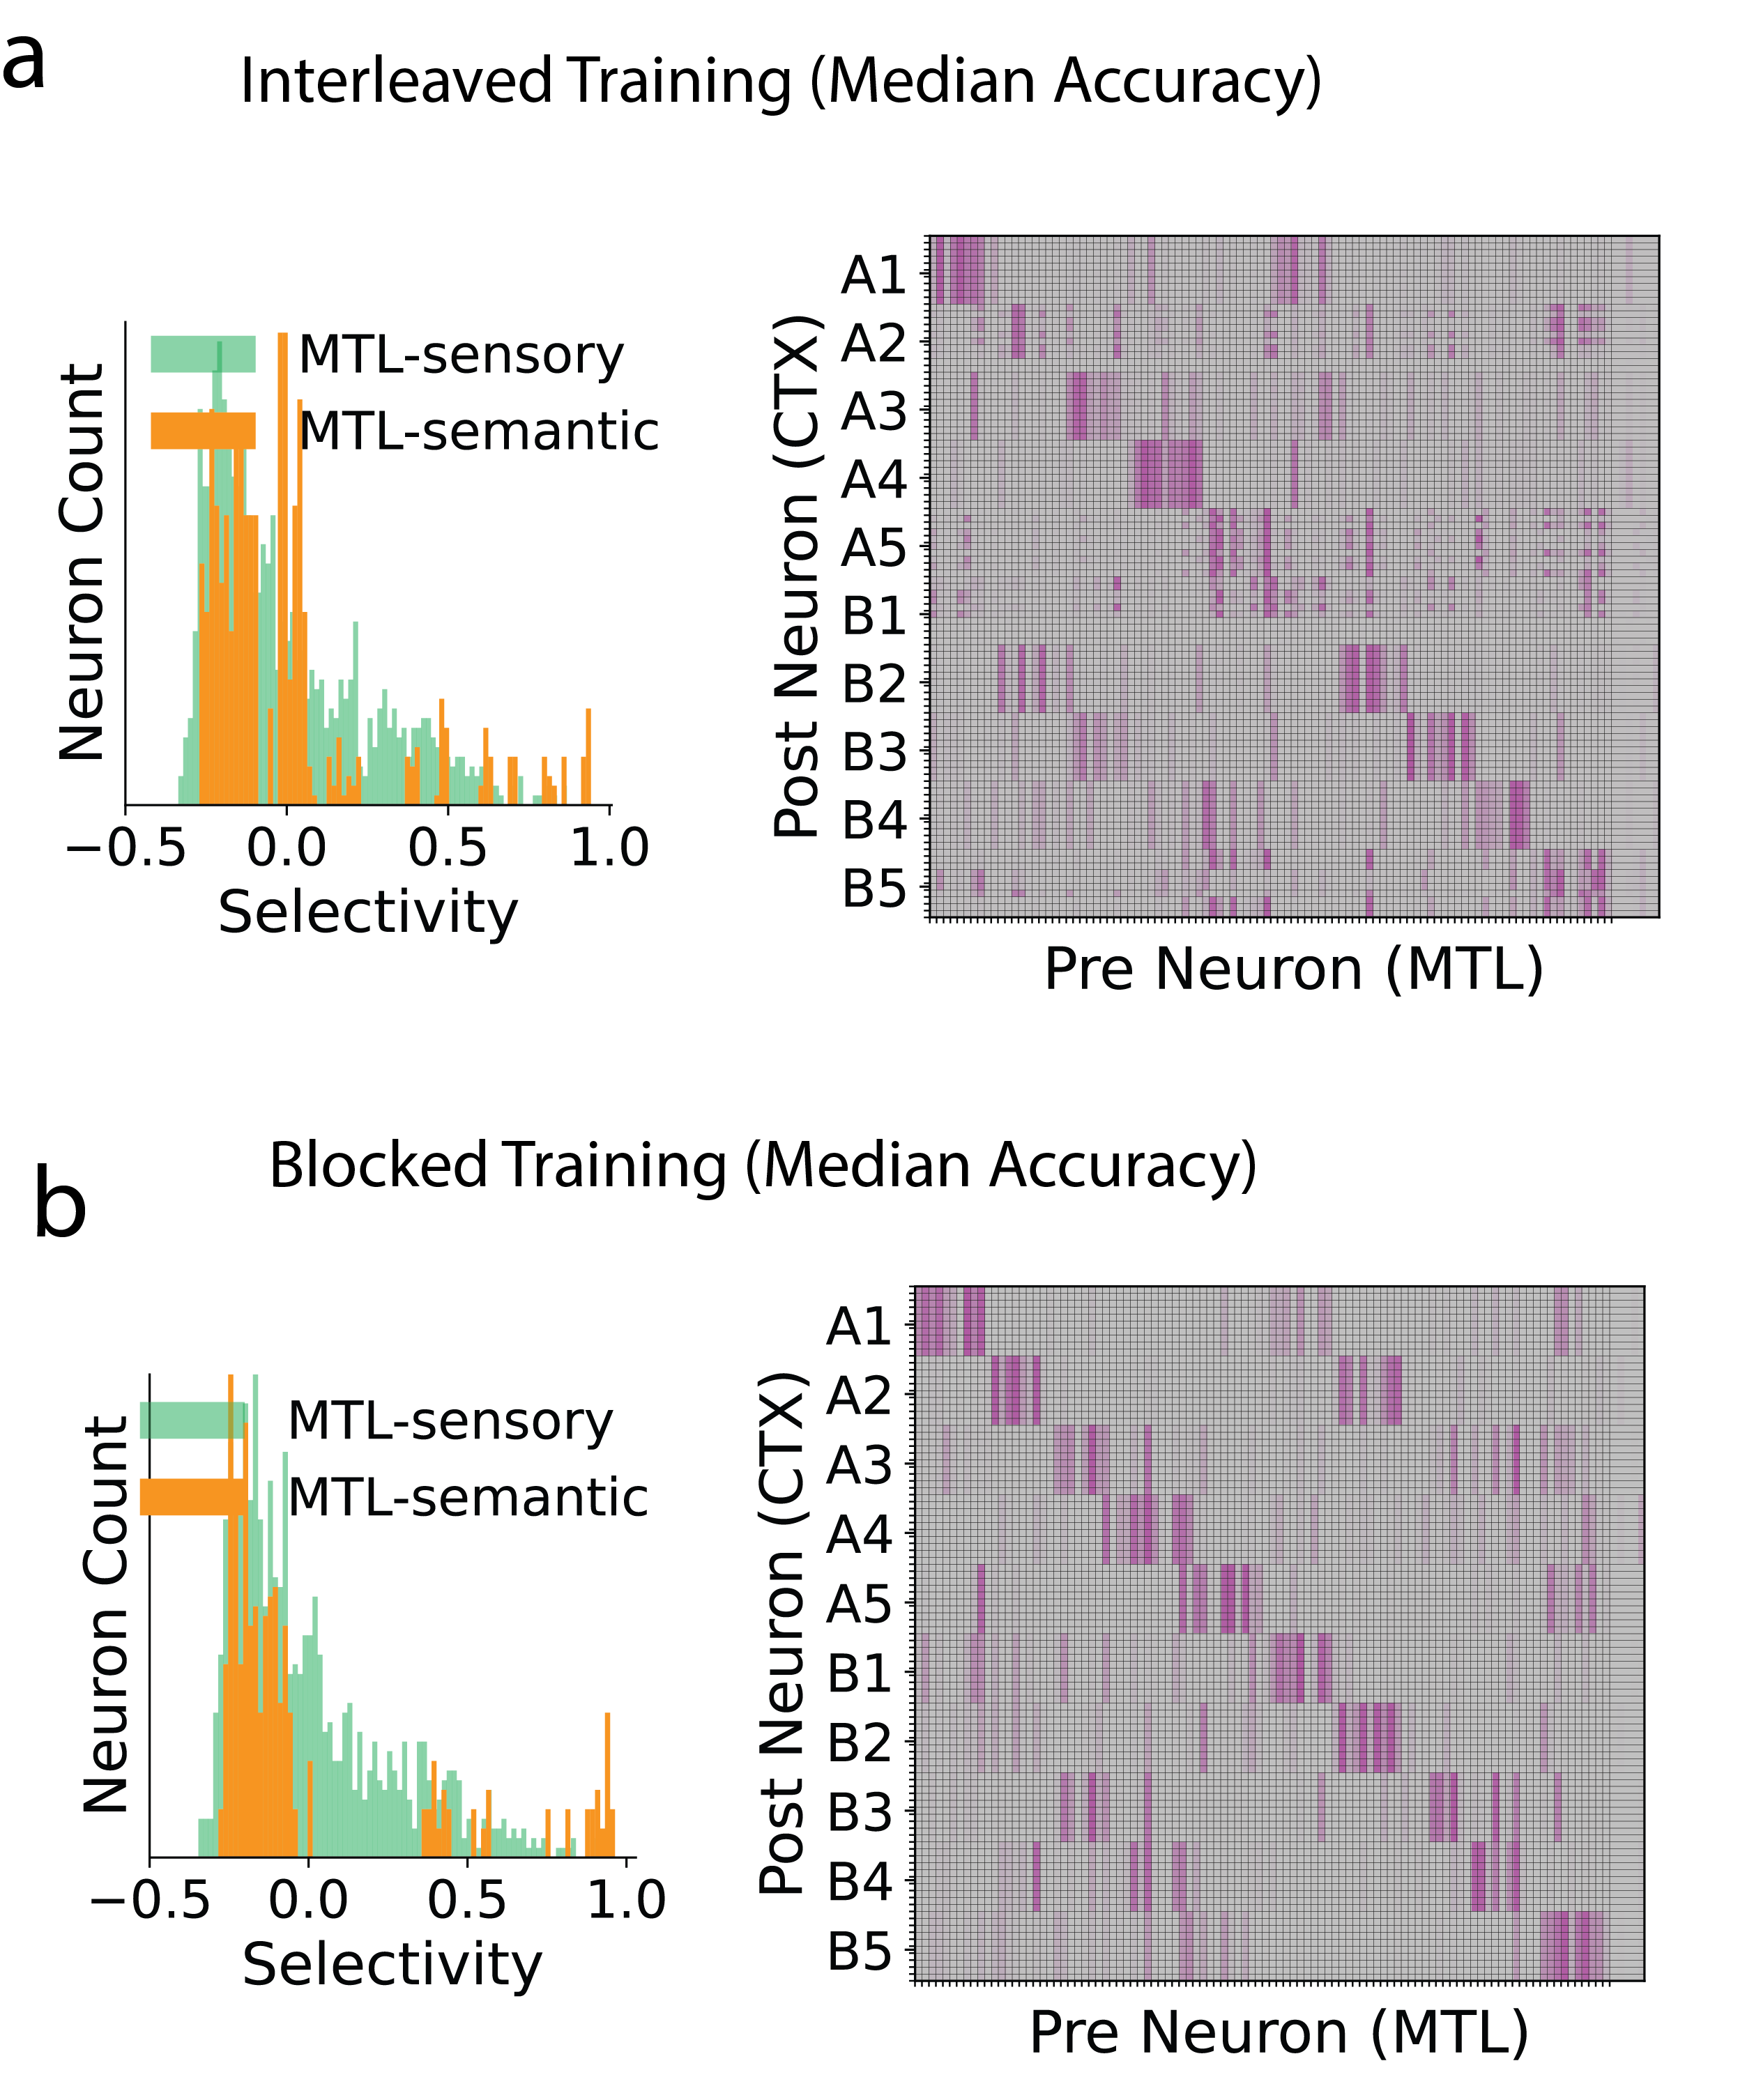
\includegraphics[width=0.65\linewidth]{Figures/Figure_5_supp.png}
    \caption{Same as Fig. \ref{fig:experimental_support_1} but for a network with median accuracy in Fig. \ref{fig:experimental_support_1}f}
    \label{fig:experimental_support_1_supp_1}
\end{figure}


\begin{figure}[h!]
    \centering
    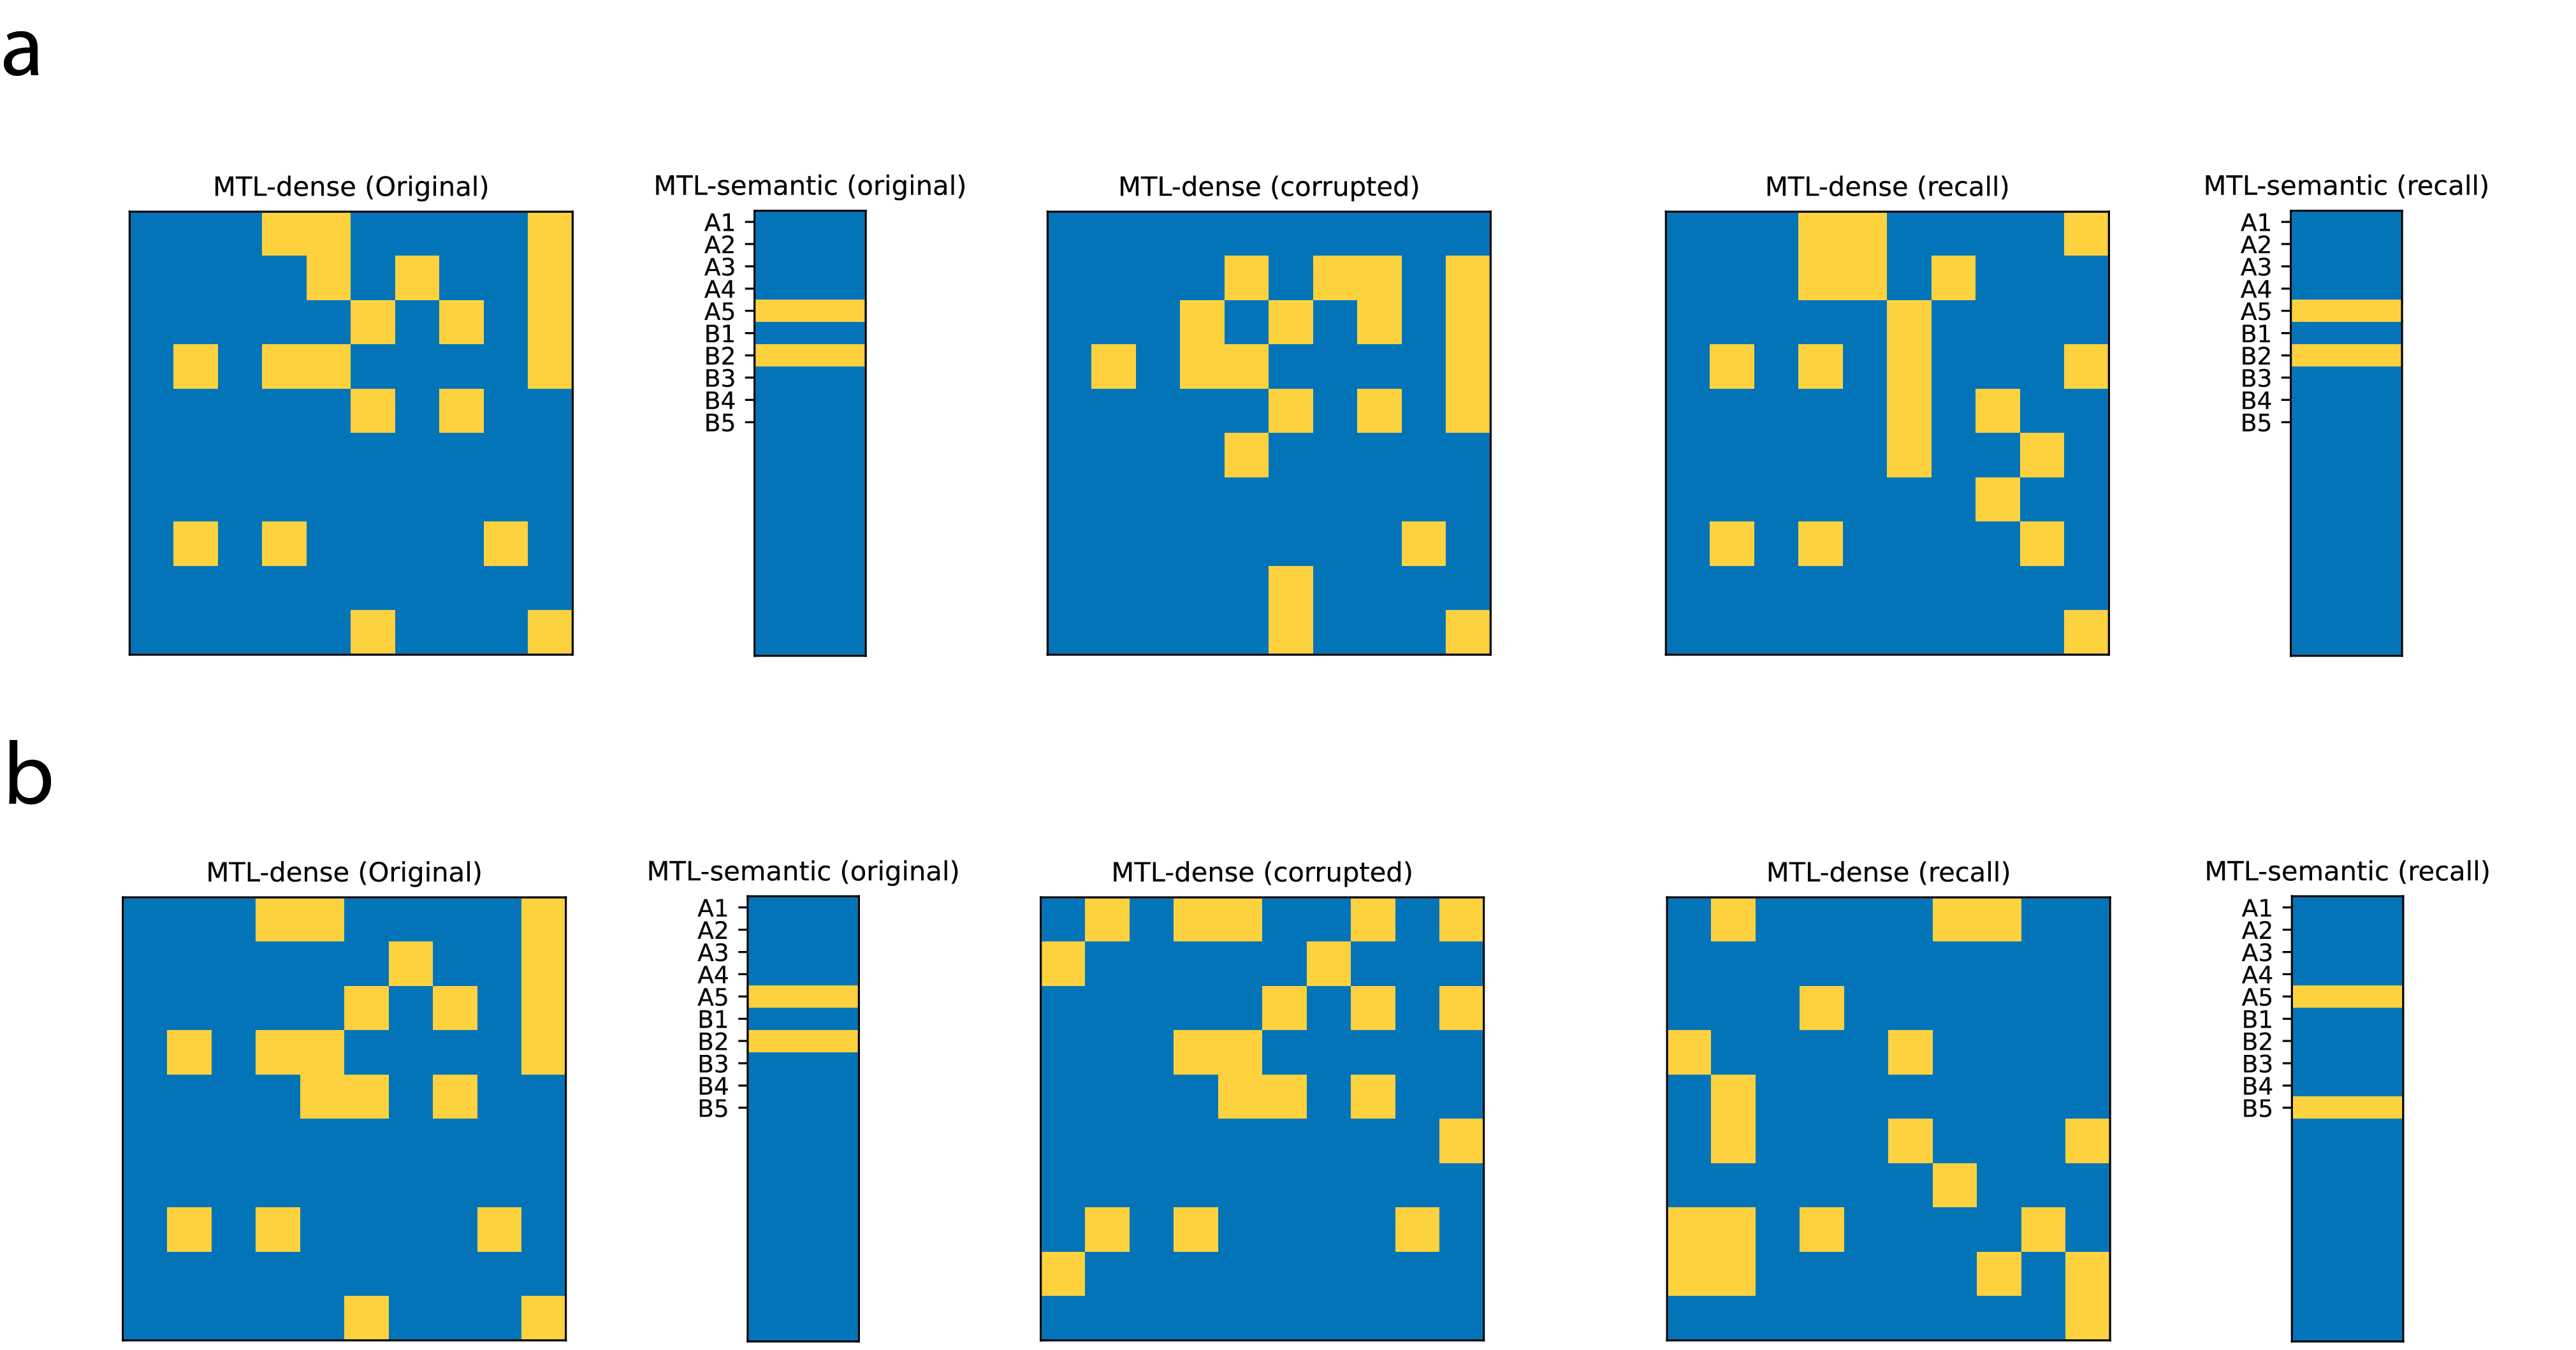
\includegraphics[width=0.95\linewidth]{Figures/Figure_6_supp_1.png}
    \caption{Example recall patterns in Fig. \ref{fig:experimental_support_1}d for only one stored episode (\textbf{A}) and 1000 stored episodes (\textbf{B}). In the limit of infinite stored patterns, a form of semantic priming leads to wrong pattern completion when the presented pattern is of the form $(A_i, B_{j\neq i})$, over-correcting it to the more likely patterns $(A_i, B_j)$ and $(A_j, B_j)$}
    \label{fig:experimental_support_2_supp_1}
\end{figure}

\begin{figure}[h!]
    \centering
    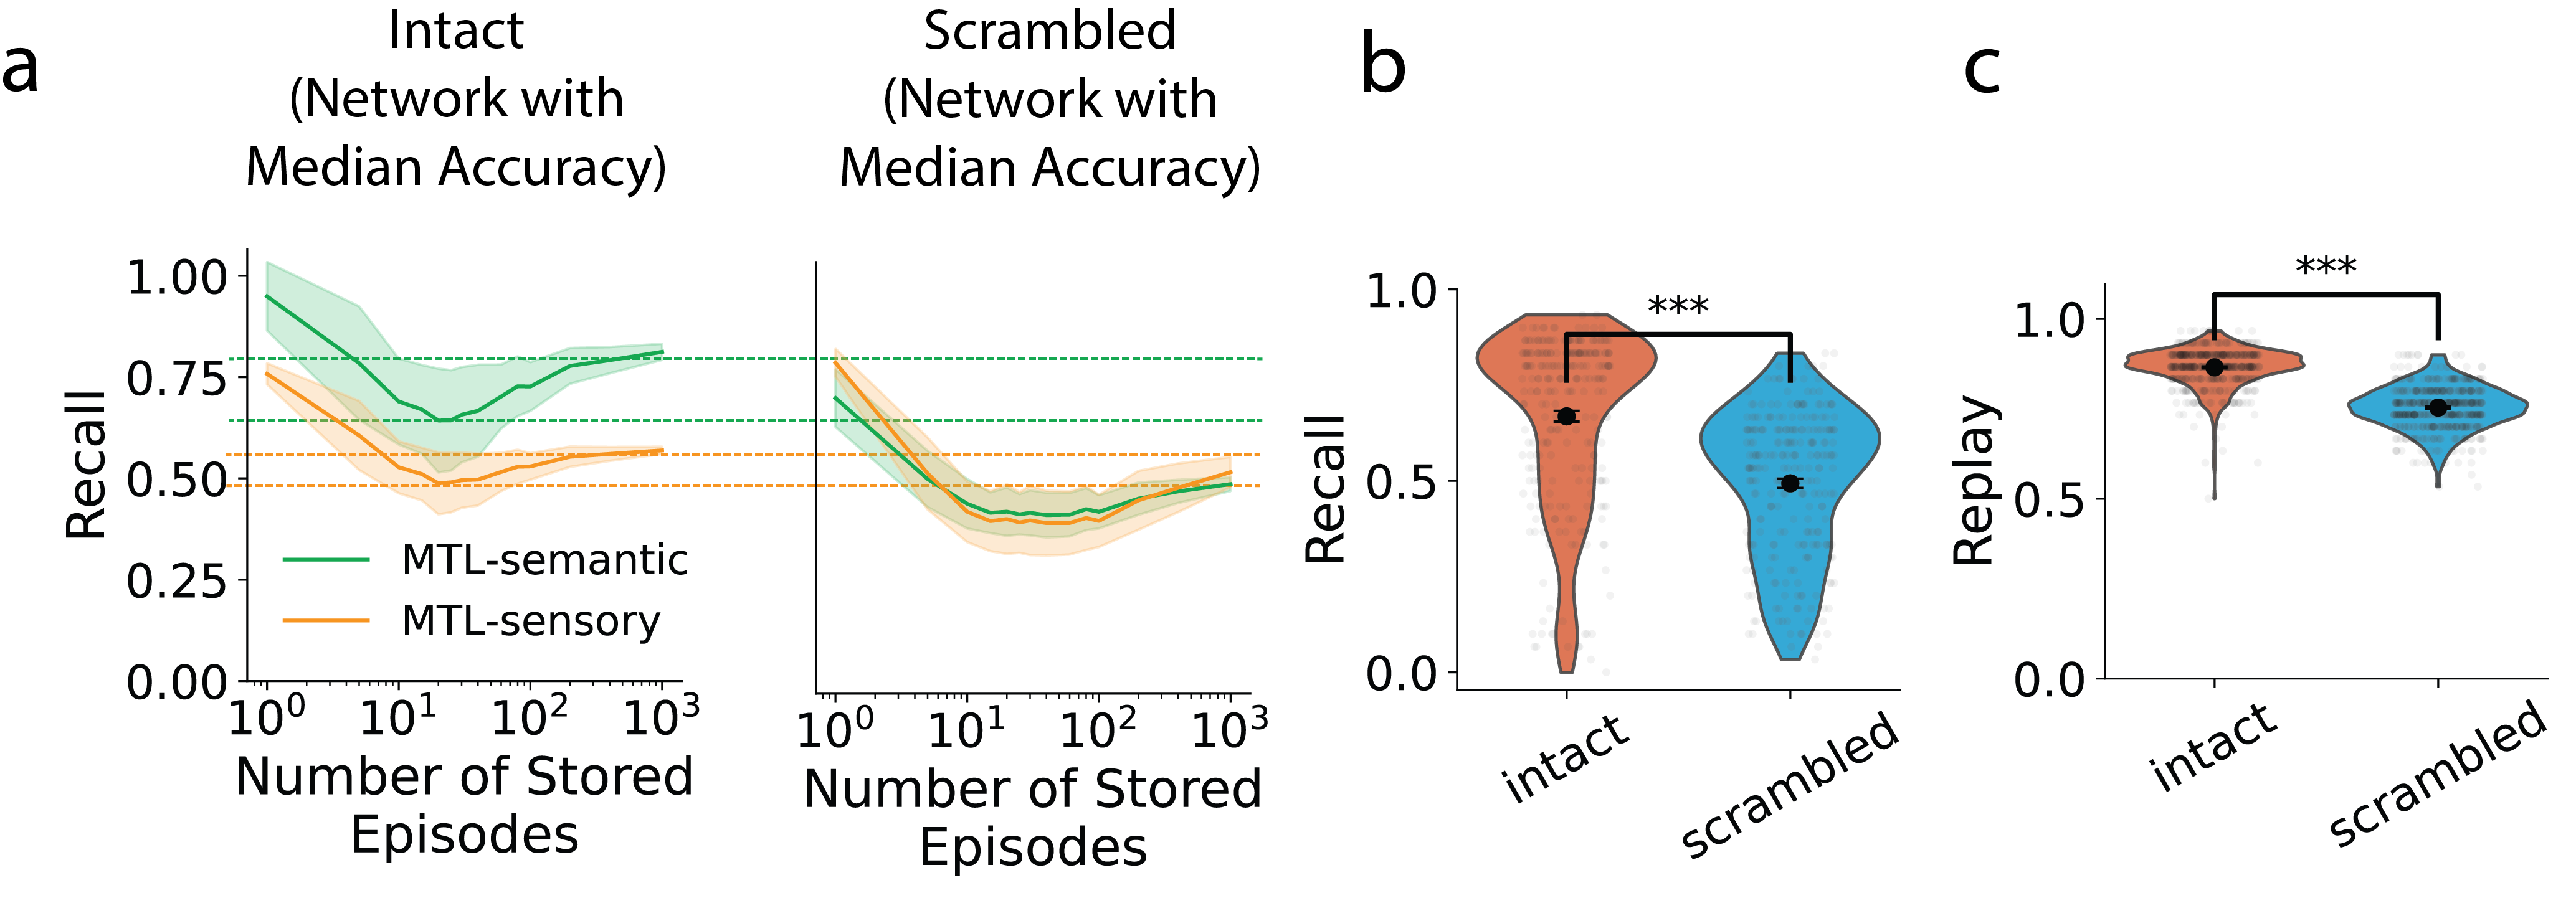
\includegraphics[width=0.95\linewidth]{Figures/Figure_6_supp_2.png}
    \caption{Same as Fig. \ref{fig:experimental_support_2} but for a network with median accuracy in Fig. \ref{fig:experimental_support_1}f}
    \label{fig:experimental_support_2_supp_2}
\end{figure}

\begin{figure}[h!]
    \centering
    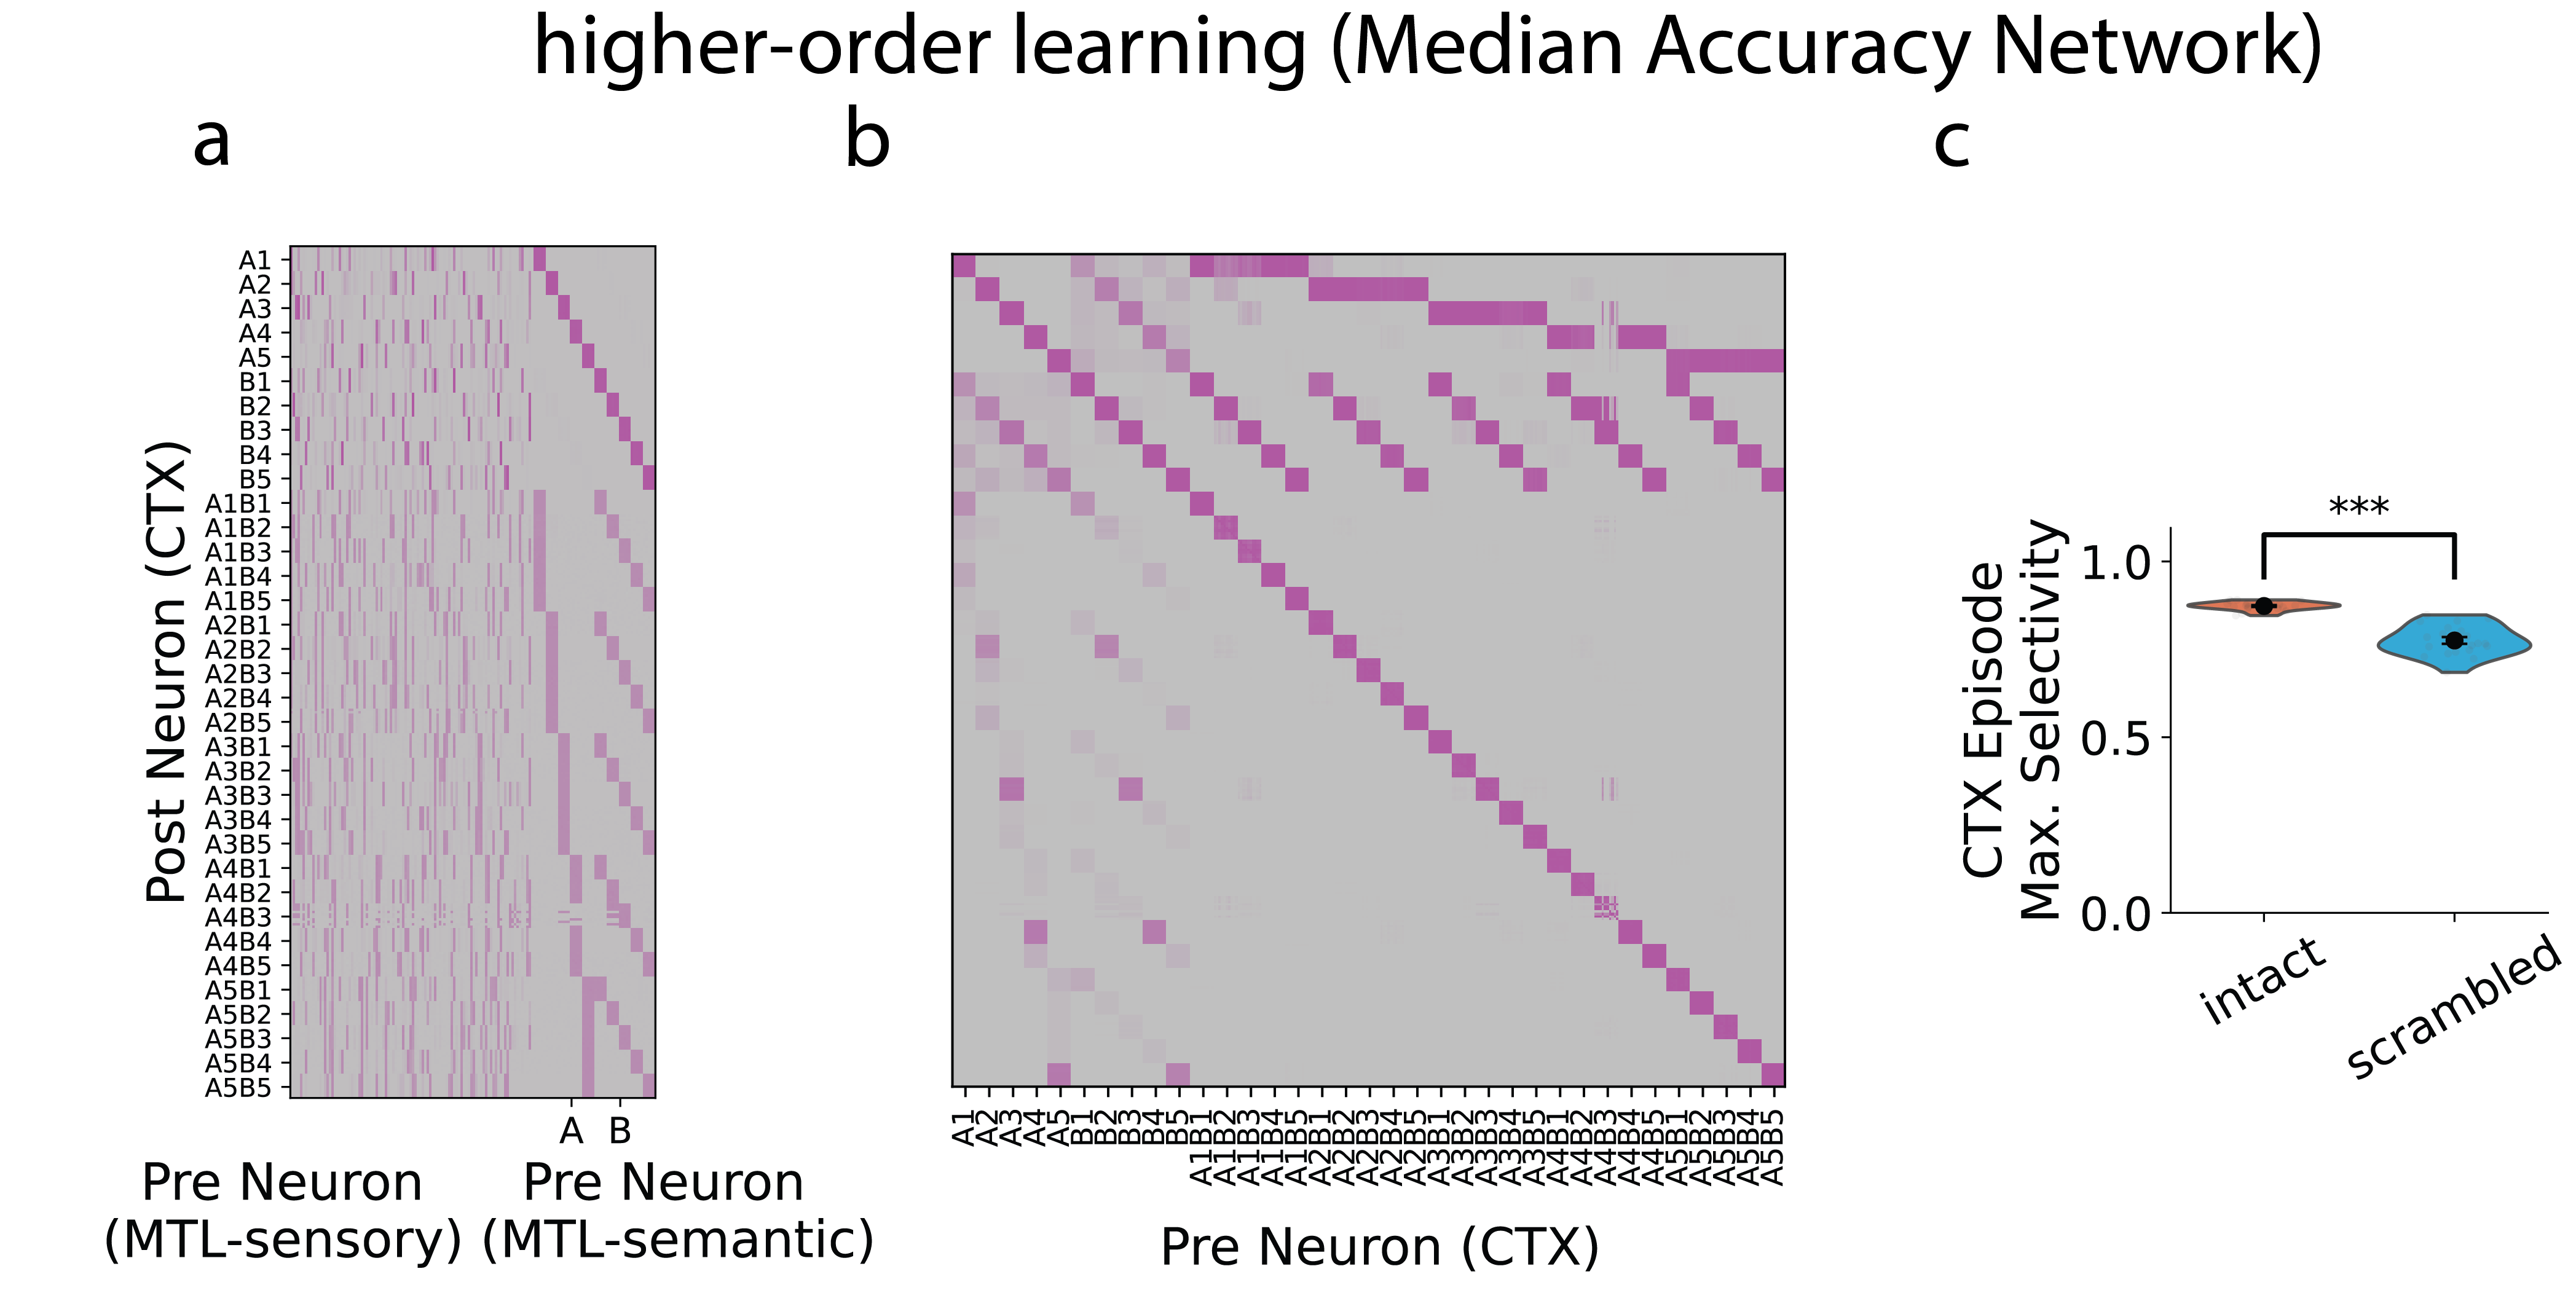
\includegraphics[width=0.95\linewidth]{Figures/Figure_7_supp.png}
    \caption{Same as Fig. \ref{fig:higher-order} but for a network with median accuracy in Fig. \ref{fig:higher-order}f}
    \label{fig:higher_order_supp}
\end{figure}
\end{document}
